\documentclass[useAMS, usenatbib, a4paper]{mnras}
\pdfsuppresswarningpagegroup=1

\usepackage{graphicx}
\usepackage{microtype}
\usepackage{xcolor}
\usepackage{fixltx2e}
\usepackage{booktabs}
\usepackage{siunitx}
\sisetup{separate-uncertainty = true}
\usepackage{color}
\usepackage{enumerate}
\usepackage{pdflscape}
\usepackage{rotating}
\usepackage{xr-hyper}
\usepackage{hyperref}
\externaldocument[Q-]{quadrics-bowshock}

\usepackage[T1]{fontenc} 
\usepackage[utf8]{inputenc}

% Fonts 
\usepackage{newtxtext}
% Note: newtxmath must come AFTER newtxtext
\usepackage[varvw,smallerops]{newtxmath}

\usepackage{chemgreek}
\activatechemgreekmapping{newtx}

\hypersetup{colorlinks=True, linkcolor=blue!50!black, citecolor=black,
  urlcolor=blue!50!black}

\usepackage{etoolbox}
\robustify\bfseries
\robustify\itshape

%% The following hack solves a problem with
%% ERROR: \pdfendlink ended up in different nesting level than \pdfstartlink.
%% See https://tex.stackexchange.com/a/249743
\makeatletter
\patchcmd\@combinedblfloats{\box\@outputbox}{\unvbox\@outputbox}{}{%
  \errmessage{\noexpand\@combinedblfloats could not be patched}%
}%
\makeatother

%% Bold italic
\newcommand\hmmax{0}            % we don't need heavy fonts
\newcommand\bmmax{1}            % reduce use of math alphabets for bold
\usepackage{bm}

%% Bundled custom packages
\usepackage{aastex-compat}

\title
{Bow shocks, bow waves, and dust waves}

\newcommand\AddressCRyA{Instituto de Radioastronom\'{\i}a y Astrof\'{\i}sica,
  Universidad Nacional Aut\'onoma de M\'exico, Apartado Postal 3-72,
  58090 Morelia, Michoac\'an, M\'exico}
\author[Henney \& Arthur]{
  William J. Henney \& S. Jane Arthur\\
  \AddressCRyA
}

% These dates will be filled out by the publisher
\date{Accepted XXX. Received YYY; in original form ZZZ}

% Enter the current year, for the copyright statements etc.
\pubyear{2019}
\DeclareMathOperator{\sgn}{sgn}
\DeclareMathOperator{\Sin}{\mathcal{S}}
\DeclareMathOperator{\Cos}{\mathcal{C}}
\DeclareMathOperator{\Cot}{\mathcal{T}}
\DeclareMathOperator{\GammaFunc}{\Gamma}
\DeclareMathOperator\erf{erf}
\newcommand\w{\ensuremath{\mathrm{w}}}
\newcommand\C{\ensuremath{\mathrm{c}}}
\providecommand{\abs}[1]{\lvert#1\rvert}
\providecommand{\Abs}[1]{\left\lvert#1\right\rvert}
\newcommand\TODO[1]{%
  \begin{center}
    \framebox{\parbox{0.8\linewidth}{
        \texttt{\footnotesize\color{red} #1}}}
  \end{center}}

\newcommand\uvec[1]{\bm{\hat{#1}}}
\newcommand\T{_{\mathrm{\scriptscriptstyle T}}}

\newcommand\Qp{\ensuremath{Q_{\text{p}}}}
\newcommand{\grain}{\ensuremath{_{\text{d}}}}
\newcommand{\B}{\ensuremath{_{\scriptscriptstyle\text{B}}}}
\newcommand{\alfven}{\ensuremath{_{\scriptscriptstyle\text{A}}}}
\newcommand{\xsec}{\ensuremath{\sigma\grain}}
\newcommand\frad{\ensuremath{f_{\text{rad}}}}
\newcommand\fmax{\ensuremath{f_{\text{max}}}}
\newcommand\thm{\ensuremath{\theta_{\text{m}}}}
\newcommand\drag{\ensuremath{_{\text{drag}}}}
\newcommand{\gas}{\ensuremath{_{\text{gas}}}}
\newcommand{\wind}{\ensuremath{_{\text{w}}}}
\newcommand{\trap}{\ensuremath{_{\text{abs}}}}
\newcommand{\ke}{\ensuremath{_{\text{kin}}}}
\newcommand{\drift}{\ensuremath{_{\text{drift}}}}
\newcommand\rad{\ensuremath{_{\text{rad}}}}
\newcommand\Lya{\ensuremath{_{\text{Ly}\alpha}}}
\newcommand\Rmin{\ensuremath{R_{\scriptscriptstyle\text{min}}}}
% Why do I need both of these?
\newcommand\sound{\ensuremath{c_{\text{s}}}}
\newcommand\soundspeed{\ensuremath{c_{\text{s,gas}}}}
\newcommand\starstar{\ensuremath{_{**}}}
\newcommand\mmp{\ensuremath{_{\text{\tiny MMP83}}}}
\newcommand\Hab{\ensuremath{_{\text{\tiny Habing}}}}
\newcommand{\thD}{\(\theta^1\)\,Ori~D}

\defcitealias{Tarango-Yong:2018a}{Paper~I}
\newcommand\PaperI{\citetalias{Tarango-Yong:2018a}}


\begin{document}
\label{firstpage}
\pagerange{\pageref{firstpage}--\pageref{lastpage}}
\maketitle
\begin{abstract}
  Dust waves and bow waves result from the action of a star's
  radiation pressure on a stream of dusty plasma that flows past it.
  They are an alternative mechanism to hydrodynamic bow shocks for
  explaining the curved arcs of infrared emission seen around some
  stars.  When gas and grains are perfectly coupled, for a broad class
  of stellar parameters, wind-supported bow shocks predominate when
  the ambient density is below \SIrange{100}{1000}{cm^{-3}}.  At
  higher densities radiation-supported bows can form, tending to be
  optically thin bow waves around B~stars, or optically thick bow
  shocks around early O~stars.  The radiation field is sufficiently
  strong to overcome the collisional coupling between grains and gas
  at a \textit{rip-point}, where the ratio of radiation pressure to
  gas pressure exceeds a critical value of roughly 1000.  When the rip
  point occurs outside the hydrodynamic bow shock, a separate dust
  wave may form, decoupled from the gas shell, which can either be
  drag-confined or inertia-confined, depending on the stream density
  and relative velocity.  In the drag-confined case, there is a
  minimum stream velocity of roughly \SI{60}{km.s^{-1}} that allows a
  steady-state stagnant drift solution for the dust wave apex.  For
  lower relative velocities, the dust dynamics close to the axis
  exhibit a limit cycle behavior (rip and snap back) between two
  different radii.  Strong coupling of charged grains to the plasma's
  magnetic field can modify these effects, but for a quasi-parallel
  field orientation the results are qualitatively similar. For a
  quasi-perpendicular field, on the other hand, the formation of a
  decoupled dust wave is strongly suppressed.
\end{abstract}

\begin{keywords}
  circumstellar matter -- radiation: dynamics -- stars: winds, outflows
\end{keywords}

\defcitealias{Tarango-Yong:2018a}{Paper~I}
\newcommand\PaperI{\citetalias{Tarango-Yong:2018a}}

\section{Introduction}
\label{sec:introduction}
\newcommand\hii{\ion{H}{ii}}

Curved emission arcs around stars \citep[e.g.,][]{Gull:1979a} are
often interpreted as \textit{bow shocks}, due to a supersonic
hydrodynamic interaction between the star's wind and an external
stream. This stream may be due to the star's own motion or to an
independent flow, such as an \hii{} region in the champagne phase
\citep{Tenorio-Tagle:1979a}, or another star's wind
\citep{Canto:1996}. However, an alternative interpretation in some
cases may be a radiation-pressure driven bow wave, as first proposed
by \citet[\S\textsc{vi}]{van-Buren:1988a}.  In this scenario, photons
emitted by the star are absorbed by dust grains in the incoming
stream, with the resultant momentum transfer being sufficient to
decelerate and deflect the grains within a certain distance from the
star, forming a dust-free, bow-shaped cavity with an enhanced dust
density at its edge.  Two regimes are possible, depending on the
strength of coupling between the gas (or plasma) and the dust.  In the
strong-coupling regime, gas--grain drag decelerates the gas along with
the dust, forming a shocked gas shell in a similar fashion to the
wind-driven bow shock case.  In the weak-coupling regime, the gas
stream is relatively unaffected and the dust temporarily decouples to
form a dust-only shell.  This second case has recently been studied in
detail in the context of the interaction of late O-type stars (which
have only weak stellar winds) with dusty photoevaporation flows inside
\hii{} regions \citep{Ochsendorf:2014a, Ochsendorf:2014b,
  Ochsendorf:2015a}.  We follow the nomenclature proposed by
\citet{Ochsendorf:2014b}, in which \textit{dust wave} refers to the
weak coupling case and \textit{bow wave} to the strong coupling case.
More complex, hybrid scenarios are also possible, such as that studied
by \citet{van-Marle:2011a}, where a hydrodynamic bow shock forms, but
the larger dust grains that accompany the stellar wind pass right
through the shocked gas shell, and form their own dust wave at a
larger radius.

\begin{figure*}
  \centering
  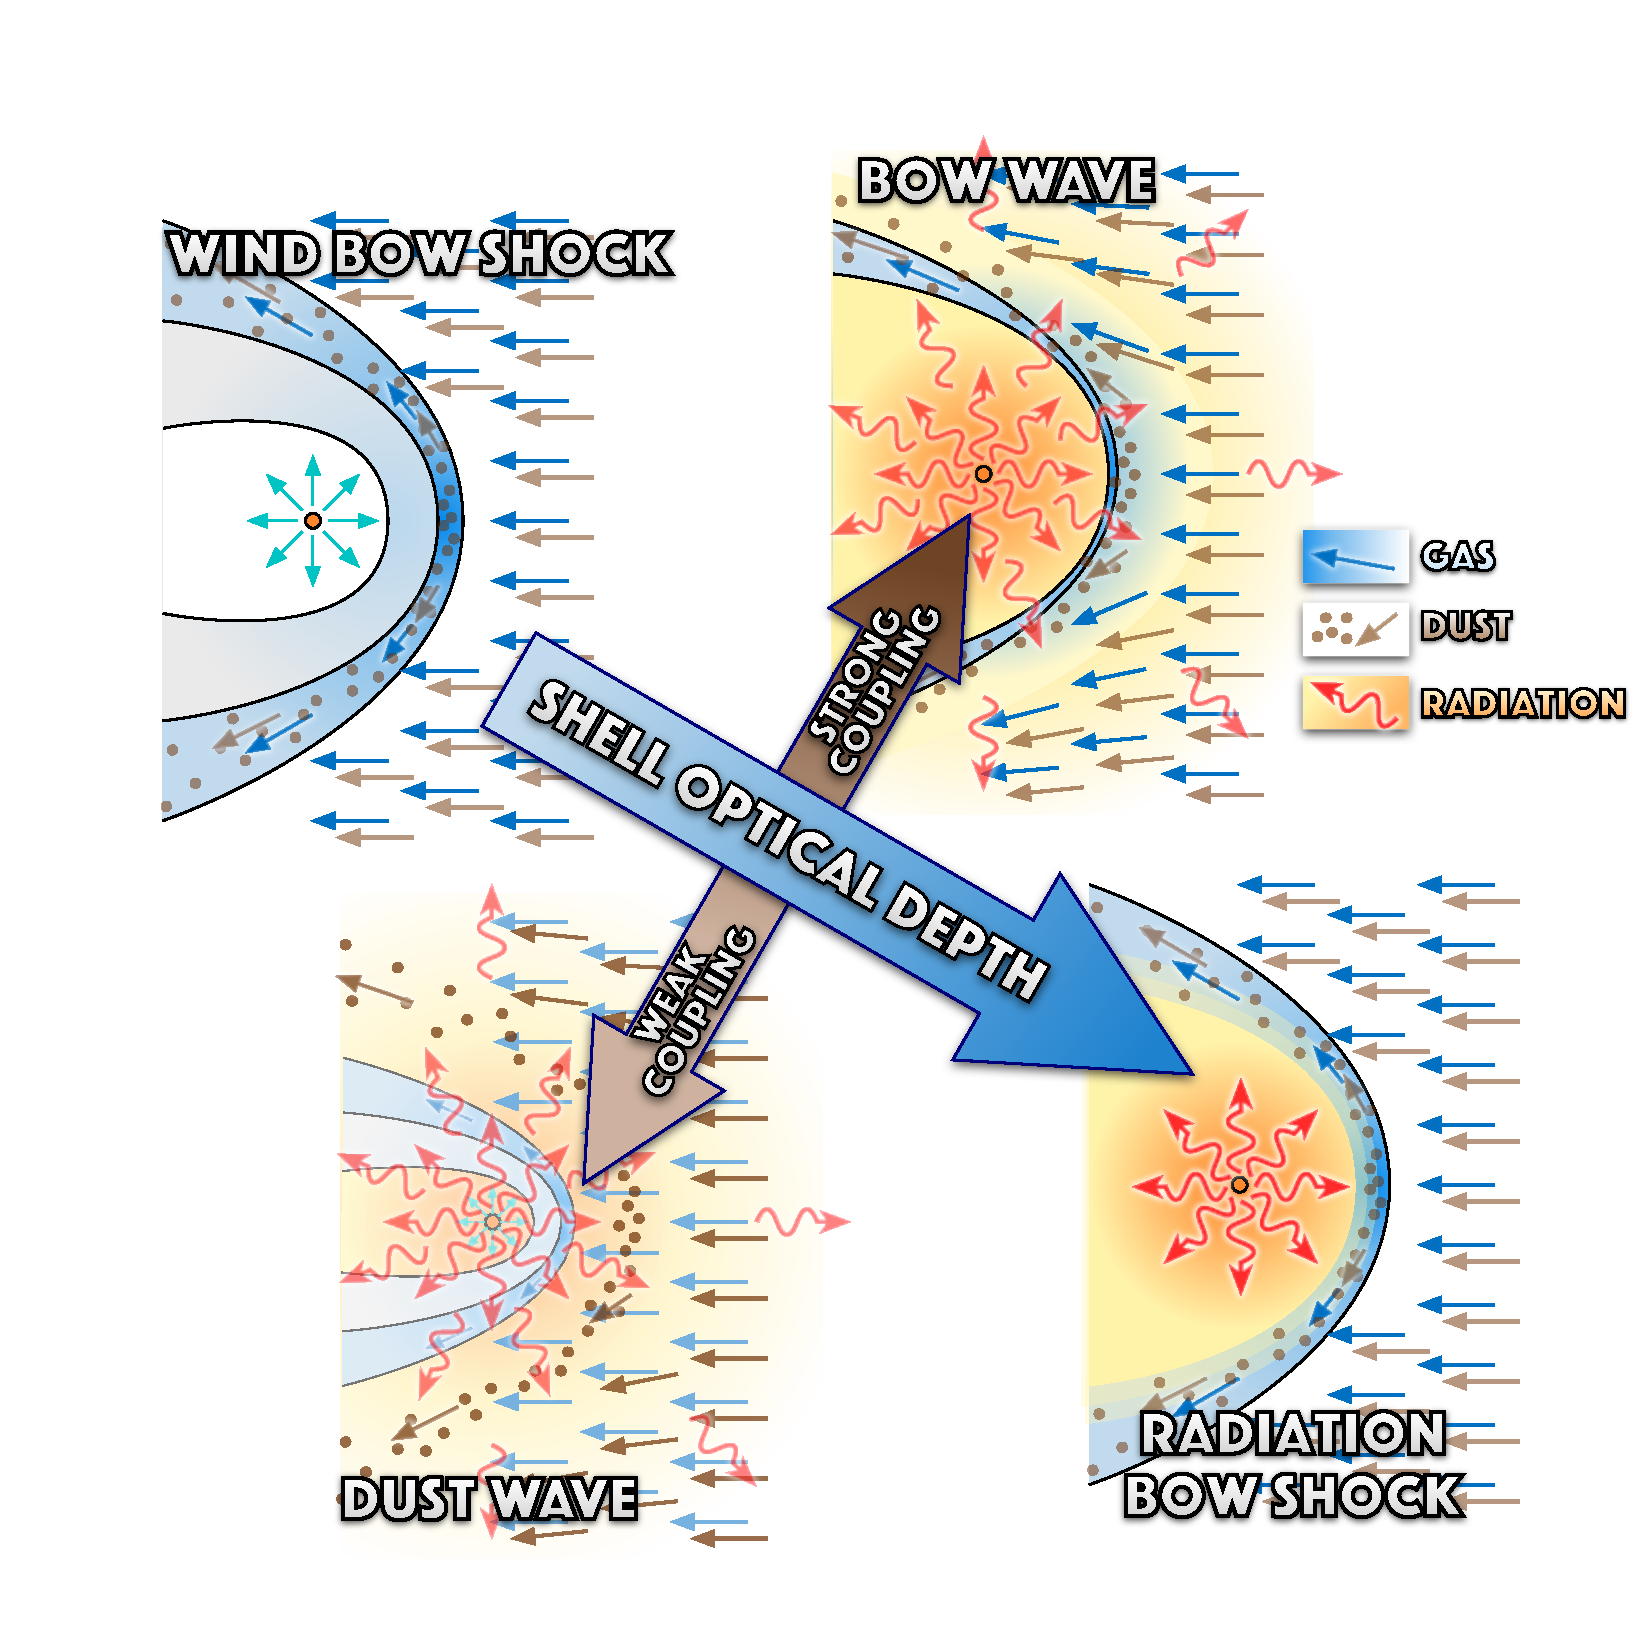
\includegraphics[width=\linewidth]{figs/bows-and-waves}
  \caption{Bow shocks, bow waves, and dust waves}
  \label{fig:3-types-bow}
\end{figure*}

In \citet[][hereafter \PaperI{}]{Tarango-Yong:2018a}, we proposed a
new two-dimensional classification scheme for bow shapes: the
projected planitude--alatude, or \(\Pi'\)--\(\Lambda'\), diagram.  Planitude
measures the flatness of the bow's apex, while alatude measures the
openness of the bow's wings.  Both are dimensionless ratios of lengths
that can be estimated from observational images.  We have analyzed the
inclination-dependent tracks on the \(\Pi'\)--\(\Lambda'\) plane for simple
geometric shapes (spheroids, paraboloids, hyperboloids) and for
thin-shell hydrodynamic bow shock models (wilkinoid, cantoids,
ancantoids).  In this paper, we will do the same for simple models of
radiation-driven dust waves (dragoids) and bow waves (trapoids).

The paper is organized as follows.
%
In \S~\ref{sec:shape-dust-wave} we do the same for simple models of a
dusty radiation bow wave (dragoids), including the effects of
gas-grain drag.
%
In \S~\ref{sec:perturbed-bows} we investigate the effects on the
planitude--alatude plane of small-amplitude perturbations to the bow
shape.
%


\section{Different types of bow}
\label{sec:different-types-bow}

\begin{figure*}
  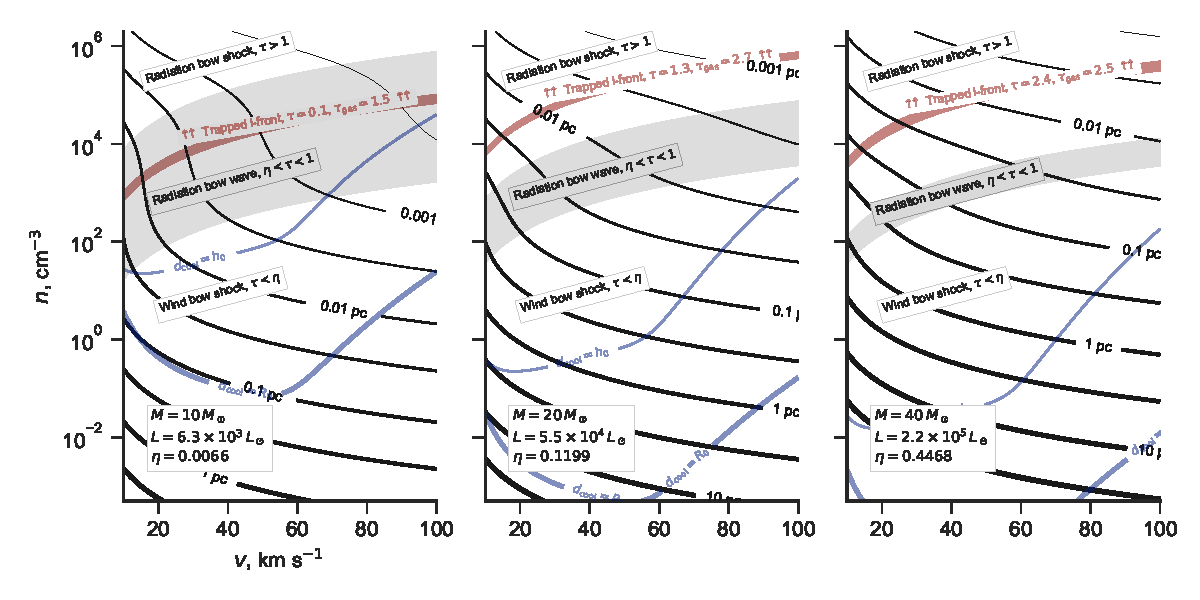
\includegraphics[width=\linewidth]{figs/zones-v-n-plane}
  \caption{Bow regimes in parameter space (\(v, n\)) of the external
    stream for main-sequence OB stars of different masses:
    (a)~\SI{10}{M_\odot}, (b)~\SI{20}{M_\odot}, (c)~\SI{40}{M_\odot}.  In all
    cases, \(\kappa = \SI{600}{cm^2.g^{-1}}\) and efficient gas-grain
    coupling is assumed. Solid black lines of varying width show the
    bow size (star-apex separation, \(R_0\)), while gray shading shows
    the radiation bow wave regime, with lower border \(\tau = \eta\) and
    upper border \(\tau = 1\), where \(\tau = 2 \kappa \rho R_0\) is the optical
    depth through the bow.  For bows above the red solid line, the
    ionization front is trapped inside the bow.  Blue lines delineate
    different cooling regimes.  Above the thin blue line
    (\(d_{\text{cool}} = h_0\)), the bow shock radiates efficiently,
    forming a thin shocked shell.  Below the thick blue line
    (\(d_{\text{cool}} = R_0\)), the bow shock is essentially
    non-radiative.}
  \label{fig:zones-v-n-plane}
\end{figure*}

In this section, we investigate the different types of bow interaction
that will occur in different regions of parameter space. We will
mainly treat the canonical case\footnote{%
  Variant cases with differing arrangements of dust and radiation
  sources are treated in \S~\ref{sec:case-inside-out}.} %
of a bow around a star of bolometric luminosity, \(L\), with a
radiatively driven wind, which is immersed in an external stream of
gas and dust with density, \(\rho\), and velocity, \(v\).  The size and
shape of the bow is determined by a generalized balance of pressure
(or, equivalently, momentum) between internal and external sources.
We assume that the stream is supersonic and super-alfvenic, so that
the external pressure is dominated by the ram pressure: \(\rho v^2\).

\subsection{Strong gas-grain coupling}
\label{sec:strong-gas-grain}

We first consider the case where the dust grains and gas are perfectly
coupled by collisions.\footnote{%
  Cases where this assumption does not hold are investigated below in
  \S~\ref{sec:imperf-coupl-betw}.} %
Although dust grains typically constitute only a small fraction
\(Z\grain \sim 0.01\) of the mass of the external stream, they
nevertheless dominate the broad-band opacity at FUV, optical and IR
wavelengths if they are present.\footnote{%
  At EUV wavelengths (\(\lambda < \SI{912}{\angstrom}\)), gas opacity
  dominates if the hydrogen neutral fraction is larger than
  \(\approx 0.001\), see discussion of ionization front trapping
  below.} %
The strong coupling assumption means that all the radiative forces
applied to the dust grains are directly felt by the gas also.

\subsubsection{Bows supported by radiation and wind}
\label{sec:three-bow-regimes}

The internal pressure is the sum of wind ram pressure and the
effective radiation pressure that acts on the bow shell.  The
radiative momentum loss rate of the star is \(L/c\) and the wind
momentum loss rate can be expressed as
\begin{equation}
  \label{eq:wind-efficiency}
  \dot{M} V = \eta L / c \ , 
\end{equation}
where \(\eta\) is the momentum efficiency of the wind, which is typically
\(< 1\) \citep{Lamers:1999b}. If the optical depth is very large, then
all of the stellar radiative momentum, emitted with rate \(L/c\), is
trapped by the bow shell.  In the single scattering limit,\footnote{%
  Although it may seem inconsistent to assume single scattering in the
  case of high optical depths, this is defensible for the following
  reasons. (1)~The grain albedo is not that high (typically
  \(\sim 0.5\) at ultraviolet through optical wavelengths). (2)~The
  scattered radiation field is more isotropic than the stellar field,
  leading to cancellation in the radiative
  flux. (3)~Absorbed radiation is re-emitted at infrared
  wavelengths, where the dust opacity is very much lower.} %
and temporarily neglecting the wind, then pressure balance at the bow
apex, a distance \(R_0\) along the symmetry axis from the star is
given by
\begin{equation}
  \label{eq:rad-press-balance-thick}
  \frac{L}{4 \pi c R_0^2} = \rho v^2 \ ,
\end{equation}
which yields a fiducial bow shock radius in this optically thick limit
as
\begin{equation}
  \label{eq:Rstar}
  R_* = \left(\frac{L}{4\pi c \rho v^2}\right)^{1/2} \ .
\end{equation}

We now consider the opposite, optically thin limit.  If the total
opacity (gas plus dust) per total mass (gas plus dust) is \(\kappa\) (with
units of \si{cm^2.g^{-1}}), then the radiative acceleration is
\begin{equation}
  \label{eq:rad-accel}
  a_{\text{rad}} = \frac{\kappa L}{4 \pi c R^2} \ .
\end{equation}
Therefore, an incoming stream with initial velocity, \(v_\infty\), can be
brought to rest by radiation alone\footnote{%
  For simplicity, we here ignore the effects of gravity, which are
  important for low ratios of \(\kappa L / M\), see
  \S~\ref{sec:effects-gravity}.  We also ignore pressure gradients and
  shocks, which are important as the velocity approaches the sound
  speed, \(\sound\) (in \S~XX below, we show that the resultant
  corrections to \(R_0\) are of order \(\sound / v_\infty\)).} %
at a distance \(R_0\) where
\begin{equation}
  \label{eq:rad-poten}
  \int_{R_0}^\infty a_{\text{rad}} \, dr = \tfrac12 v_\infty^2 \ , 
\end{equation}
yielding
\begin{equation}
  \label{eq:rad:R0}
  R_0 = \frac{\kappa L}{2\pi c v_\infty^2} \ .
\end{equation}
On the other hand, we can also argue as in the optically thick case
above by approximating the bow shell as a surface, and balancing
stellar radiation pressure against the ram pressure of the incoming
stream.  The important difference when the shell is not optically
thick is that only a fraction \(1 - e^{-\tau}\) of the radiative momentum
is absorbed by the bow, so that
equation~\eqref{eq:rad-press-balance-thick} is replaced with
\begin{equation}
  \label{eq:rad-press-balance-tau}
  \frac{L (1 - e^{-\tau})}{4 \pi c R_0^2} = \rho v^2 \ .
\end{equation}
In the optically thin limit, \(1 - e^{-\tau} \approx \tau\), so these two
descriptions can be seen to agree so long as
\begin{equation}
  \label{eq:tau-thin}
  \tau = 2 \kappa \rho R_0 \ ,
\end{equation}
which we will assume to hold generally.

Then, defining a fiducial optical depth,
\begin{equation}
  \label{eq:tau-star}
  \tau_* = \rho \kappa R_* \ ,
\end{equation}
and adding in the stellar wind ram pressure\footnote{%
  We implicitly assume that the interaction of the stellar wind with
  the external stream can always be treated in the continuum limit.
  This will be true if either the collisional mean free path or the
  ion Larmor radius is much smaller than \(R_0\), which is almost
  always the case.} %
from equation~\eqref{eq:wind-efficiency}, we find that the general bow
radius can be written in terms of the fiducial radius as
\(R_0 = x R_*\), where \(x\) is the solution of
\begin{equation}
  \label{eq:rad-full-x}
  x^2 - \bigl(1 - e^{-2 \tau_* x} \bigr) - \eta = 0 \ .
\end{equation}
Since this is a transcendental equation, \(x\) must be found
numerically, but we can write explicit expressions for three limiting
cases:
\begin{equation}
  \label{eq:x-cases}
  x \approx
  \begin{cases}
    \text{if \(\tau_* \gg 1\):} & (1 + \eta)^{1/2}  \\
    \text{if \(\tau_*^2 \ll 1\):} & \tau_* + \bigl( \tau_*^2 + \eta \bigr)^{1/2} \approx
    \begin{cases}
      \text{if \(\tau_*^2 \gg \eta\):} & 2 \tau_*  \\
      \text{if \(\tau_*^2 \ll \eta\):} & \eta^{1/2} 
    \end{cases}
  \end{cases}
\end{equation}
The first case, \(x \approx (1 + \eta)^{1/2}\), corresponds to a
\textit{radiation bow shock}; the second case,
\(x \approx 2 \tau_* \), corresponds to a \textit{radiation bow wave}; and the
third case, \(x \approx \eta^{1/2}\), corresponds to a \textit{wind bow shock}.
The two bow shock cases are similar in that the external stream is
oblivious to the presence of the star until it suddenly hits the bow
shock shell, differing only in whether it is radiation or wind that is
providing the internal pressure.  In the intermediate bow wave case,
on the other hand, the external stream is gradually decelerated by
absorption of photons as it approaches the bow.\footnote{A shock does
  still form in this case, but shocked material constitutes only a
  fraction of the total column density of the shell, see
  \S~\ref{sec:shape-bow-wave}.}

\begin{table*}
  \centering
  \caption{Stellar parameters for example stars}
  \label{tab:stars}
  \begin{tabular}{l S S S S S S S S S l}
    \toprule
    & {\(M / \si{M_\odot}\)} & {\(L_4\)}
    & {\(\dot{M}_{-7}\)} & {\(V_3\)} & {\( \eta \)}
    & {Sp.~Type} 
    & {\(T_{\text{eff}} / \si{kK}\)} & {\(\lambda_{\text{eff}}\) / \si{\um}}
    & {\(S_{49}\)} & Figures 
    \\
    \midrule
    & 10 & 0.63 & 0.0034 & 2.47 & 0.0066 & {B1.5\,V} & 25.2 & 0.115 & 0.00013
                   & \ref{fig:zones-v-n-plane}a,
                     \ref{fig:decouple-v-n-plane},
                     \ref{fig:decouple-v40-versus-n} \\
    Main-sequence OB stars
    & 20 & 5.45 & 0.492 & 2.66 & 0.1199 & {O9\,V} & 33.9 & 0.086 & 0.16
                   & \ref{fig:zones-v-n-plane}b\\
    & 40 & 22.2 & 5.1 & 3.31 & 0.4468 & {O5\,V} & 42.5 & 0.068 & 1.41
                   & \ref{fig:zones-v-n-plane}c\\[\smallskipamount]
    Blue supergiant star
    & 33 & 30.2 & 20.2 & 0.93 & 0.3079 & {B0.7\,Ia} & 23.5 & 0.123 & 0.016
                   & \ref{fig:B-supergiant} \\[\smallskipamount]
    Red supergiant star
    & 20 & 15.6 & 100 & 0.015 & 0.0476 & {M1\,Ia} & 3.6 & 0.805 & 0
                   & \ref{fig:M-supergiant} \\ 
    \bottomrule
  \end{tabular}
\end{table*}

We now consider the application to bow shocks around main sequence OB
stars, expressing stellar and ambient parameters in terms of typical
values as follows:
\begin{align*}
  \label{eq:stellar-parameters}
  \dot{M}_{-7} &= \dot{M} / \bigl(\SI{e-7}{M_\odot.yr^{-1}}\bigr) \\
  V_3 &= V / \bigl(\SI{1000}{km.s^{-1}}\bigr) \\
  L_4 &= L / \bigl(\SI{e4}{L_\odot}\bigr) \\
  v_{10} &= v_\infty / \bigl( \SI{10}{km.s^{-1}} \bigr) \\
  n &= (\rho / \bar{m}) / \bigl( \SI{1}{cm^{-3}} \bigr) \\
  \kappa_{600} &= \kappa / \bigl( \SI{600}{cm^2.g^{-1}} \bigr) \ ,
\end{align*}
where \(\bar{m}\) is the mean mass per hydrogen nucleon
(\(\bar{m} \approx 1.3 m_{\text{p}} \approx \SI{2.17e-24}{g}\) for solar
abundances).  Note that \(\kappa = \SI{600}{cm^2.g^{-1}}\) corresponds to a
cross section of \(\approx \SI{e-21}{cm^2}\) per hydrogen nucleon, which is
typical for interstellar medium dust \citep{Bertoldi:1996a} at far
ultraviolet wavelengths, where OB stars emit most of their radiation.
In terms of these parameters, we can express the stellar wind momentum
efficiency as
\begin{equation}
  \label{eq:wind-eta-typical}
  \eta = \num{0.495} \,\dot{M}_{-7} \,V_3  \,L_4^{-1}
\end{equation}
and the fiducial radius and optical depth as
\begin{align}
  \label{eq:Rstar-typical}
  R_* / \si{pc} &= \num{2.21} \, (L_4 / n)^{1/2} \,v_{10}^{-1} \\
  \label{eq:taustar-typical}
  \tau_* &= \num{0.0089} \,\kappa_{600} \, (L_4 \,n)^{1/2} \,v_{10}^{-1} \ .
\end{align}
In Figure~\ref{fig:zones-v-n-plane}, we show results for the bow size
(apex distance, \(R_0\)) as a function of the density, \(n\), and
relative velocity, \(v_\infty\), of the external stream, with each panel
corresponding to a particular star, with parameters as shown in
Table~\ref{tab:stars}.  To facilitate comparison with previous work,
we choose stellar parameters similar to those used in the
hydrodynamical simulations of \citet{Meyer:2014b, Meyer:2016a,
  Meyer:2017a}, based on stellar evolution tracks for stars of
\SIlist{10;20;40}{M_\odot} \citep{Brott:2011a} and theoretical wind
prescriptions \citep{de-Jager:1988a, Vink:2000a}.  Although the
stellar parameters do evolve with time, they change relatively little
during the main-sequence lifetime of several million years.\footnote{%
  \label{fn:meyer-velocities-too-low}
  Note that we have recalculated the stellar wind terminal velocities,
  since the values given in the \citeauthor{Meyer:2014b} papers are
  troublingly low.  We have used the prescription
  \(V = 2.6 V_{\text{esc}}\), where
  \(V_{\text{esc}} = \left( 2 G M (1 - \Gamma_e)/ R \right)^{1/2}\) is the
  photospheric escape velocity, which is appropriate for strong
  line-driven winds with \(T_{\text{eff}} > \SI{21 000}{K}\)
  \citep{Lamers:1995a}.  We find velocities of
  \SIrange{2500}{3300}{km.s^{-1}}, which are consistent with
  observations and theory \citep{Vink:1999a} for O~stars, but at least
  two times higher than those cited by \citet{Meyer:2014b}. For
  main-sequence B~stars, wind column densities are too low to reliably
  measure the terminal velocity from near ultraviolet P~Cygni profiles
  \citep{Prinja:1989a}, and so the values are theory-dependent
  \citep{Krticka:2014a} and hence more uncertain.  A further
  complication is the existence of a subset of OB stars with
  anomalously weak winds \citep{Puls:2008a}, which in some cases is
  related to the presence of strong (\(\sim \SI{1}{kG}\)) magnetic fields
  \citep{Oskinova:2011b}.} %
The three examples are an early B~star (\SI{10}{M_\odot}), a late O~star
(\SI{20}{M_\odot}), and an early O~star (\SI{40}{M_\odot}), which cover the
range of luminosities and wind strengths expected from bow-producing
hot main sequence stars.  The luminosity is a steep function of
stellar mass (\(L \sim M^{2.5}\)) and the wind mass-loss rate is a steep
function of luminosity (\(\dot{M} \sim L^{2.2}\)), which means that the
wind momentum efficiency is also a steep function of mass
(\(\eta \sim M^3\)), approaching unity for early O~stars, but falling to
less than 1\% for B~stars.

\begin{figure}
  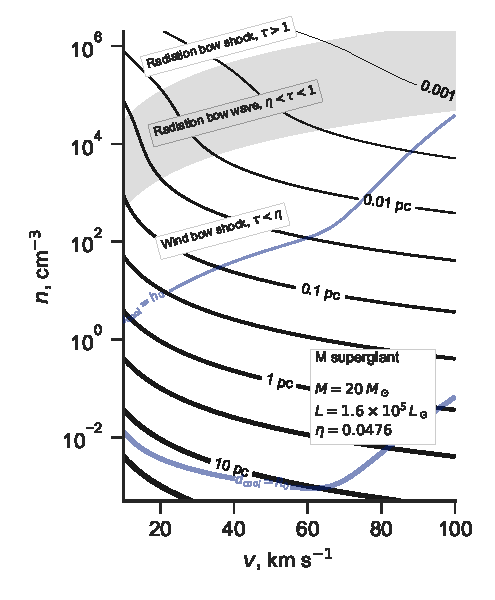
\includegraphics[width=\linewidth]{figs/zones-v-n-plane-RSG}
  \caption{As Fig.~\ref{fig:zones-v-n-plane}, but for a cool M-type
    supergiant instead of hot main sequence stars.  A smaller dust
    opacity is used, \(\kappa = \SI{60}{cm^2.g^{-1}}\), because of the
    reduced extinction efficiency at the optical/infrared wavelengths
    emitted by this star.}
  \label{fig:M-supergiant}
\end{figure}

It can be seen from Figure~\ref{fig:zones-v-n-plane} that the onset of
the radiation bow wave regime is very similar for the three
main-sequence stars, occurring at
\(n > \text{\numrange{20}{40}} \, v_{10}^2\).  An important
difference, however, is that for the \SI{40}{M_\odot} star, which has a
powerful wind, the radiation bow wave regime only occurs for a very
narrow range of densities, whereas for the \SI{10}{M_\odot} star, with a
much weaker wind, the regime is much broader, extending to
\(n < \num{e4} \, v_{10}^2\).  Another difference is the size scale of
the bows in this regime, which is
\(R_0 = \text{\SIrange{0.001}{0.003}{pc}}\) for the \SI{10}{M_\odot} star
if \(v_\infty = \SI{40}{km.s^{-1}}\), but \(R_0 \approx \SI{0.1}{pc}\) for the
\SI{40}{M_\odot} star, assuming the same inflow velocity.

Figure~\ref{fig:M-supergiant} shows results for a cool M-type
super-giant star with stellar parameters inspired by Betelgeuse
(\chemalpha~Orionis), as listed in Table~\ref{tab:stars}.  Unlike the
UV-dominated spectrum of the hot stars, this star emits predominantly
in the near-infrared, where the dust extinction efficiency is lower,
so we adopt a lower opacity of \SI{60}{cm^2.g^{-1}}.  This has the
effect of shifting the radiation bow wave regime to higher densities:
\(n = \text{\numrange{1000}{30 000}}\, v_{10}^2\) in this case.


\subsubsection{Effects of stellar gravity}
\label{sec:effects-gravity}

In principle, gravitational attraction from the star, of mass \(M\),
will partially counteract the radiative acceleration.  This can be
accounted for by replacing \(L\) with an effective luminosity
\newcommand\Edd{\ensuremath{_{\text{E}}}}
\begin{equation}
  \label{eq:effective-luminosity}
  L_{\text{eff}} = L \bigl(1 - \Gamma\Edd^{\,-1}\bigr) \ ,
\end{equation}
in which \(\Gamma\Edd\) is the Eddington factor:
\begin{equation}
  \label{eq:eddington-factor}
  \Gamma\Edd = \frac{\kappa L}{4\pi c G M} = 458.5 \, \frac{\kappa_{600} L_4}{ M } \ ,
\end{equation}
where, in the last expression, \(M\) is measured in solar masses.  For
the stars in Table~\ref{tab:stars}, we find
\(\Gamma\Edd \approx \text{\numrange{30}{400}}\), so gravity can be safely
ignored.  The only exception is when the optical depth of the bow is
very large: \(\tau > \ln\Gamma\Edd \sim 5\), in which case gravity may be
important in the outer parts of the shell (see
\citealt{Rodriguez-Ramirez:2016b}).



\subsubsection{Ionization state of the bow shell}
\label{sec:trapp-ioniz-front}

\newcommand\alphaB{\ensuremath{\alpha_{\text{B}}}}
\newcommand\shell{\ensuremath{_{\text{sh}}}}

\begin{figure}
  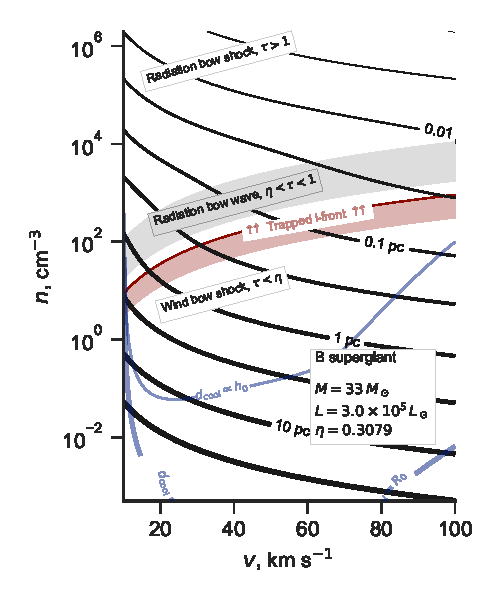
\includegraphics[width=\linewidth]{figs/zones-v-n-plane-BSG}
  \caption{As Fig.~\ref{fig:zones-v-n-plane}, but for an evolved
    B-type supergiant instead of main sequence stars.  This is similar
    to the early O MS star of Fig.~\ref{fig:zones-v-n-plane}\textit{c}
    in many respects, except for the trapping of the ionization front,
    which occurs for much lower outer stream densities.}
  \label{fig:B-supergiant}
\end{figure}

In this section we calculate whether the star is capable of
photoionizing the entire bow shock shell, or whether the ionization
front will be trapped within it.  The number of hydrogen
recombinations\footnote{%
  The diffuse field is treated in the on-the-spot approximation,
  assuming all emitted Lyman continuum photons are immediately
  re-absorbed locally, so the case~B recombination co-efficient,
  \(\alphaB = \num{2.6e-13}\, T_4^{-0.7}\, \si{cm^3.s^{-1}}\), is
  used, where \(T_4 = T/\SI{e4}{K}\).} %
per unit time per unit area in a fully ionized shell is
\begin{equation}
  \label{eq:shell-recombination-rate}
  \mathcal{R} = \alphaB n\shell^2 h\shell \ ,
\end{equation}
while the advective flux of hydrogen nuclei through the shock is 
\begin{equation}
  \label{eq:shell-advective-flux}
  \mathcal{A} = n v \ ,
\end{equation}
and the flux of hydrogen-ionizing photons
(\(h \nu > \SI{13.6}{eV}\)) incident on the inner edge of the shell is
\begin{equation}
  \label{eq:shell-ionizing-flux}
  \mathcal{F} = \frac{S} {4 \pi R_0^2} \ , 
\end{equation}
where \(S\) is the ionizing photon luminosity of the star.  Any shell
with \(\mathcal{R} + \mathcal{A} > \mathcal{F}\) cannot be entirely
photoionized by the star, and so must have trapped the ionization
front.

The ratio of advective particle flux to ionizing flux is, from
equations~\eqref{eq:Rstar}, \eqref{eq:shell-advective-flux},
\eqref{eq:shell-ionizing-flux},
\begin{equation}
  \label{eq:advective-over-ionizing-flux}
  \frac{\mathcal{A}}{\mathcal{F}} = \num{5.86e-5} \frac{x^2 L_4}{v_{10} S_{49}} \ , 
\end{equation}
which is nearly always small.  For clarity of exposition, we therefore
ignore \(\mathcal{A}\) in the following discussion, although it is
included in quantitative calculations.  The column density of the
shocked shell can be found, for example, from equations~(10) and~(12)
of \citet{Wilkin:1996a} in the limit \(v_\infty/V \to 0\) (Wilkin's parameter
\(\alpha\)) and \(\theta \to 0\).  This yields
\begin{equation}
  \label{eq:shocked-shell-column}
  n\shell h\shell = \tfrac34 n R_0 \ .
\end{equation}
Assuming strong cooling behind the shock,\footnote{%
  This is shown to be justified in \S~\ref{sec:radi-cool-lengths}.
} %
the shell density is
\begin{equation}
  \label{eq:isothermal-shell-density}
  n\shell = \mathcal{M}_0^2 n \,
\end{equation}
where
\(\mathcal{M}_0 = v_\infty / \sound\) is the isothermal Mach number of the
external stream.\footnote{%
  \label{fn:temperature-dependence}
  The sound speed depends on the temperature and hydrogen and helium
  ionization fractions, \(y\) and \(y_{\text{He}}\) as
  \(\sound^2 = (1 + y + z_{\text{He}} y_{\text{He}}) (k T /
  \bar{m})\), where \(z_{\text{He}}\) is the helium nucleon abundance
  by number relative to hydrogen and
  \(k = \SI{1.3806503e-16}{erg.K^{-1}}\) is Boltzmann's constant.  We
  assume \(y = 1\), \(y_{\text{He}} = 0.5\), \(z_{\text{He}} = 0.09\),
  so that \(\sound = \num{11.4}\, T_4^{1/2}\, \si{km.s^{-1}}\). } %
Putting these together with equations~\eqref{eq:Rstar} and
~\eqref{eq:tau-star}, one finds that \(\mathcal{R} > \mathcal{F}\)
implies
\begin{equation}
  \label{eq:ifront-trap-x-cubed-taustar}
  x^3 \tau_* > \frac{4 S c \sound \bar{m}^2 \kappa}{3 \alpha L} \ .
\end{equation}
From equation~\eqref{eq:rad-full-x}, it can be seen that \(x\) depends
on the external stream parameters, \(n\), \(v_\infty\) only via
\(\tau_*\), and so equation~\eqref{eq:ifront-trap-x-cubed-taustar} is a
condition for \(\tau_*\), which, by using
equation~\eqref{eq:taustar-typical}, becomes a condition on
\(n / v_{10}^2\).  In the radiation bow shock case,
\(x = (1 + \eta)^{1/2}\), and the condition can be written:
\begin{equation}
  \label{eq:ifront-trap-density-RBS}
  \frac{n}{v_{10}^2} > \num{2.65e8} \, \frac{S_{49}^2 T_4^{3.4}}{L_4^3 (1 + \eta)^3} \ , 
\end{equation}
where
\begin{equation*}
  S_{49} = S / \bigl( \SI{e49}{s^{-1}} \bigr) \ .
\end{equation*}
Numerical values of \(S_{49}\) for our three example stars are given
in Table~\ref{tab:stars}, taken from Figure~4 of
\citet{Sternberg:2003a}.  In the radiation bow wave case,
\(x = 2\tau_*\), and the condition can be written:
\begin{equation}
  \label{eq:ifront-trap-taustar-RBW}
  \frac{n}{v_{10}^2} > \num{5.36e4} \, \frac{S_{49}^{1/2} T_4^{0.85} }{\kappa_{600}^{3/2} L_4^{3/2}} \ . 
\end{equation}
In the wind bow shock case, the result is the same as
equation~\eqref{eq:ifront-trap-density-RBS}, but changing the factor
\((1 + \eta)^3\) to \(\eta^3\).  For the example hot stars in
Table~\ref{tab:stars}, and assuming \(\kappa_{600} = 1\),
\(T_4 = 0.8\), the resulting density threshold is
\(n > (\text{\numrange{1000}{5000}})\, v_{10}^2\), depending only
weakly on the stellar parameters, which is shown by the red lines in
Figure~\ref{fig:zones-v-n-plane}.  For the \SI{10}{M_\odot} star, this is
in the radiation bow wave regime, whereas for the higher mass stars it
is in the radiation bow shock regime.  When the external stream is
denser than this, then the outer parts of the shocked shell may be
neutral instead of ionized, giving rise to a cometary compact \hii{}
region \citep{Mac-Low:1991a, Arthur:2006a}.  This is only necessarily
true, however, when the star is isolated.  If the star is in a cluster
environment, then the contribution of other nearby massive stars to
the ionizing radiation field must be considered.

Quite different results are obtained for a B-type supergiant star (see
Tab.~\ref{tab:stars} and Fig.~\ref{fig:B-supergiant}), which has a
similar bolometric luminosity and wind strength to the \SI{40}{M_\odot}
main-sequence star, but a hundred times lower ionizing luminosity.
This results in a far lower threshold for trapping the ionization
front of \(n > 40 v_{10}^2\).  The advective flux, \(\mathcal{A}\), is
relatively stronger for this star than for the main-sequence stars, but
even for \(v_{10} < 2\), where the effect is strongest, the change is
only of order the width of the dark red line in
Figure~\ref{fig:B-supergiant}.


In principle, when the ionization front trapping occurs in the bow
wave regime, then the curves for \(R_0\) will be modified in the
region above the red line because all of the ionizing radiation is
trapped in the shell due to gas opacity, which is not included in
equation~\eqref{eq:tau-thin}.  However, this only happens for our
\SI{10}{M_\odot} star, which has a relatively soft spectrum.
Table~\ref{tab:stars} gives the peak wavelength of the stellar
spectrum for this star as \(\lambda_{\text{eff}} = \SI{0.115}{\um}\), which
is significantly larger than the hydrogen ionization threshold at
\SI{0.0912}{\um}, meaning that only a small fraction of the total
stellar luminosity is in the EUV band and affected by the gas opacity.
The effect on \(R_0\) is therefore small.  For the higher mass stars,
\(\lambda_{\text{eff}} < \SI{0.0912}{\um}\), so the majority of the
luminosity is in the EUV band, but in these cases the ionization front
trapping occurs well inside the radiation bow shock zone, where the
dust optical depth is already sufficient to trap all of the radiative
momentum.

\subsubsection{Radiative cooling lengths}
\label{sec:radi-cool-lengths}
\newcommand\M{\ensuremath{\mathcal{M}}}
In this section, we calculate whether the radiative cooling is
sufficiently rapid behind the bow shock to allow the formation of a
thin, dense shell.  Since cooling is least efficient at low densities,
we will assume that the wind bow shock regime applies unless otherwise
specified. We label quantities just outside the shock by the subscript
``0'', quantities just inside the shock (after thermalization, but
before any radiative cooling) by the subscript ``1'', and quantities
after the gas has cooled back to the photoionization equilibrium
temperature by the subscript ``2''.  Assuming a ratio of specific
heats, \(\gamma = 5/3\), the relation between the pre-shock and immediate
post-shock quantities is
\begin{align}
  % \M_1 &= \left(\frac{\M_0^2 + 3} {5\M_0^2 - 1}\right)^{1/2} \\
  \label{eq:shock-n-jump}
  \frac{n_1}{n_0} &= \frac{4 \M_0^2} {\M_0^2 + 3} \\
  \label{eq:shock-T-jump}
  \frac{T_1}{T_0} &= \tfrac1{16} \bigl( 5\M_0^2 - 1 \bigr) \bigl( 1 + 3/\M_0^2 \bigr) \\
  \label{eq:shock-v-jump}
  \frac{v_1}{v_0} &= \left(\frac{n_1}{n_0}\right)^{-1} \ ,
\end{align}
where \(\M_0 = v_0 / \sound\).  The cooling length of the post-shock
gas can be written as
\newcommand\cool{\ensuremath{_{\text{cool}}}}
\begin{equation}
  \label{eq:dcool}
  d\cool = \frac{3 P_1 v_1} { 2 \bigl(  \mathcal{L}_1 - \mathcal{G}_1 \bigr) }\ ,  
\end{equation}
where \(P_1\) is the thermal pressure and \(\mathcal{L}_1\),
\(\mathcal{G}_1\) are the volumetric radiative cooling and heating
rates.  For fully photoionized gas, we have
\(P_1 \approx 2 n_1 k T_1\), \(\mathcal{L}_1 = n_1^2 \Lambda(T_1)\), and
\(\mathcal{G}_1 = n_1^2 \Gamma(T_1)\), where \(\Lambda(T)\) is the cooling
coefficient, which is dominated by metal emission lines that are
excited by electron collisions, and \(\Gamma(T)\) is the heating
coefficient, which is dominated by hydrogen photo-electrons
\citep{Osterbrock:2006a}. The cooling coefficient has a maximum around
\SI{e5}{K}, and for typical ISM abundances can be approximated as
follows:
\begin{align}
  \label{eq:cooling-coefficient}
  \Lambda_{\text{warm}} &= \num{3.3e-24} \, T_4^{2.3} \, \si{erg.cm^{-3}.s^{-1}}\\
  \Lambda_{\text{hot}} &= \num{e-20} \, T_4^{-1}\, \si{erg.cm^{-3}.s^{-1}} \\
  \Lambda &= \left( \Lambda_{\text{warm}}^{-k} +  \Lambda_{\text{hot}}^{-k} \right)^{-1/k}
      \quad \text{with} \quad k = 3 \ ,
\end{align}
which is valid in the range \(0.7 < T_4 < 1000\).  We approximate the heating coefficient as
\begin{equation}
  \label{eq:heating-coefficient}
  \Gamma = \num{1.77e-24} \, T_4^{-1/2} \, \si{erg.cm^{-3}.s^{-1}} \ ,
\end{equation}
where the coefficient is chosen so as to give \(\Gamma = \Lambda\) at
an equilibrium temperature of \(T_4 = 0.8\).

In Figure~\ref{fig:zones-v-n-plane} we show curves calculated from
equations~\eqref{eq:shock-n-jump} to~\eqref{eq:heating-coefficient},
corresponding to \(d\cool = R_0\) (thick blue line) and
\(d\cool = h_0\) (thin blue line), where \(h_0\) is the shell
thickness in the efficient cooling case.  In this context, \(n_0 = n\)
and \(n_2 = n\shell\), so that \(h_0\) follows from
equations~\eqref{eq:shocked-shell-column}
and~\eqref{eq:isothermal-shell-density} as
\begin{equation}
  \label{eq:strong-cooling-h0}
  h_0 = \tfrac34 \M_0^{-2} R_0 \ .
\end{equation}
The bends in the curves at \(v \approx \SI{50}{km.s^{-1}}\) are due to the
maximum in the cooling coefficient \(\Lambda(T)\) around
\(\SI{e5}{K}\).  For bows with outer stream densities above the thin
blue line, radiative cooling is so efficient that the bow shock can be
considered isothermal, and so the shell is dense and thin (at least,
in the apex region).  It can be seen that the ionization front
trapping always occurs at densities larger than this, which justifies
the use of equation~\eqref{eq:isothermal-shell-density} in the
previous section.  For bows with outer stream densities below the
thick blue line, cooling is unimportant and the bow shock can be
considered non-radiative.  In this case the shell is thicker than in
the radiative case,
\(h\shell/R_0 \approx \text{\numrange{0.2}{0.3}}\).\footnote{%
  An approximate value can be found from
  equation~\eqref{eq:shocked-shell-column} by substituting \(n = n_0\)
  and \(n\shell \approx n_1\), then using equation~\eqref{eq:shock-n-jump}.
  Consideration of the slight increase in density between the shock
  and the contact discontinuity reduces this value by 5--10\%.} %
For bows with outer stream densities between the two blue lines,
cooling does occur, albeit inefficiently, so that the shell thickness
is set by \(d\cool\) rather than \(h_0\).

\subsection{Imperfect coupling between gas and dust}
\label{sec:imperf-coupl-betw}

\begin{figure}
  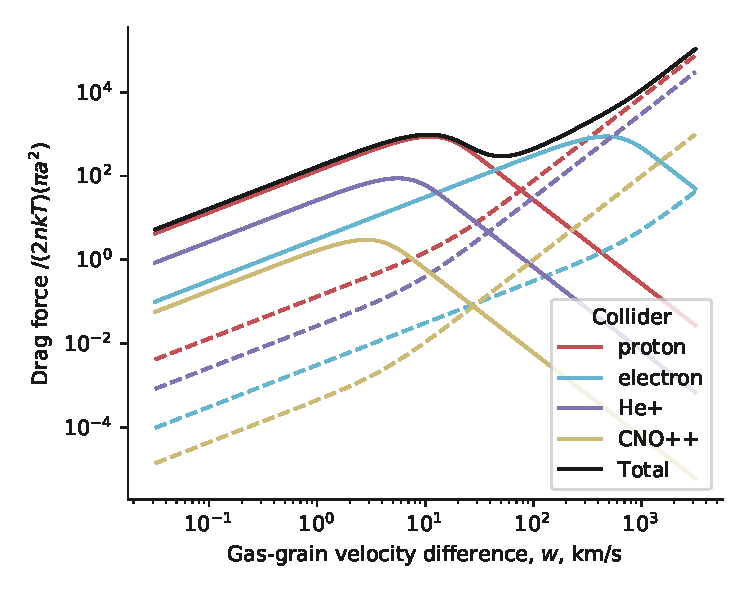
\includegraphics[width=\linewidth]{figs/test-Fdrag-components}
  \caption{Contributions of different collider species to the
    dimensionless drag force, \(f\drag / f_*\), as a function of
    gas--grain slip velocity, \(w\).  Solid lines show the Coulomb
    (electrostatic) drag, while dashed lines show the Epstein
    (solid-body) drag.  Results are shown for dimensionless grain
    potential \(\phi = 10\).  All Coulomb forces scale with
    \(\phi^2\), while the Epstein forces are independent of \(\phi\).  The
    species labelled ``CNO++'' represents the combined effect of all
    metals (see footnote~\ref{fn:metal-drag}).}
  \label{fig:drag-components}
\end{figure}


\begin{figure}
  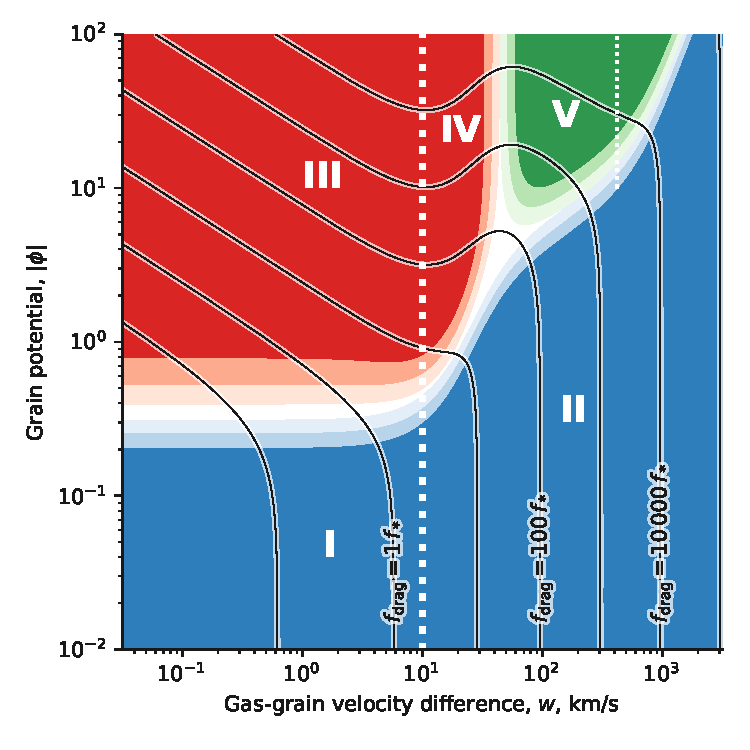
\includegraphics[width=\linewidth]{figs/test-Fdrag-param-space}
  \caption{Regimes of gas--grain drag as a function of slip velocity
    and grain potential.  The different regimes are indicated by bold
    roman numerals, as explained in
    Table~\ref{tab:fdrag-regimes}. Blue shading indicates regions
    dominated by Epstein (solid-body) drag, whereas red and green
    shading indicate regions dominated by Coulomb drag due to protons
    and electrons, respectively.  In each case, the saturated color
    represents a contribution \(> 70\%\) of the relevant component to
    the total drag force, while progressively lighter shading
    represents the \(> 60\%\) and \(> 50\%\) levels.  The thick white
    dotted line indicates the transition between the subthermal and
    superthermal regimes for protons, while the thin white dotted line
    indicates the corresponding transition for electrons.  Contours
    show the total drag force in units of \(f_*\) (see
    eq.~[\ref{eq:fstar}]) in decade intervals from \(0.1\) to
    \(10^4\), as labelled.  Results are shown for
    \(T = \SI{8000}{K}\) and \(n = \SI{100}{cm^{-3}}\), but the
    differences are very slight throughout the ranges
    \(T = \text{\SIrange{5000}{15000}{K}}\) and
    \(n = \text{\SIrange{e-3}{e6}{cm^{-3}}}\).}
  \label{fig:drag-v-phi-plane}
\end{figure}


\begin{figure*}
  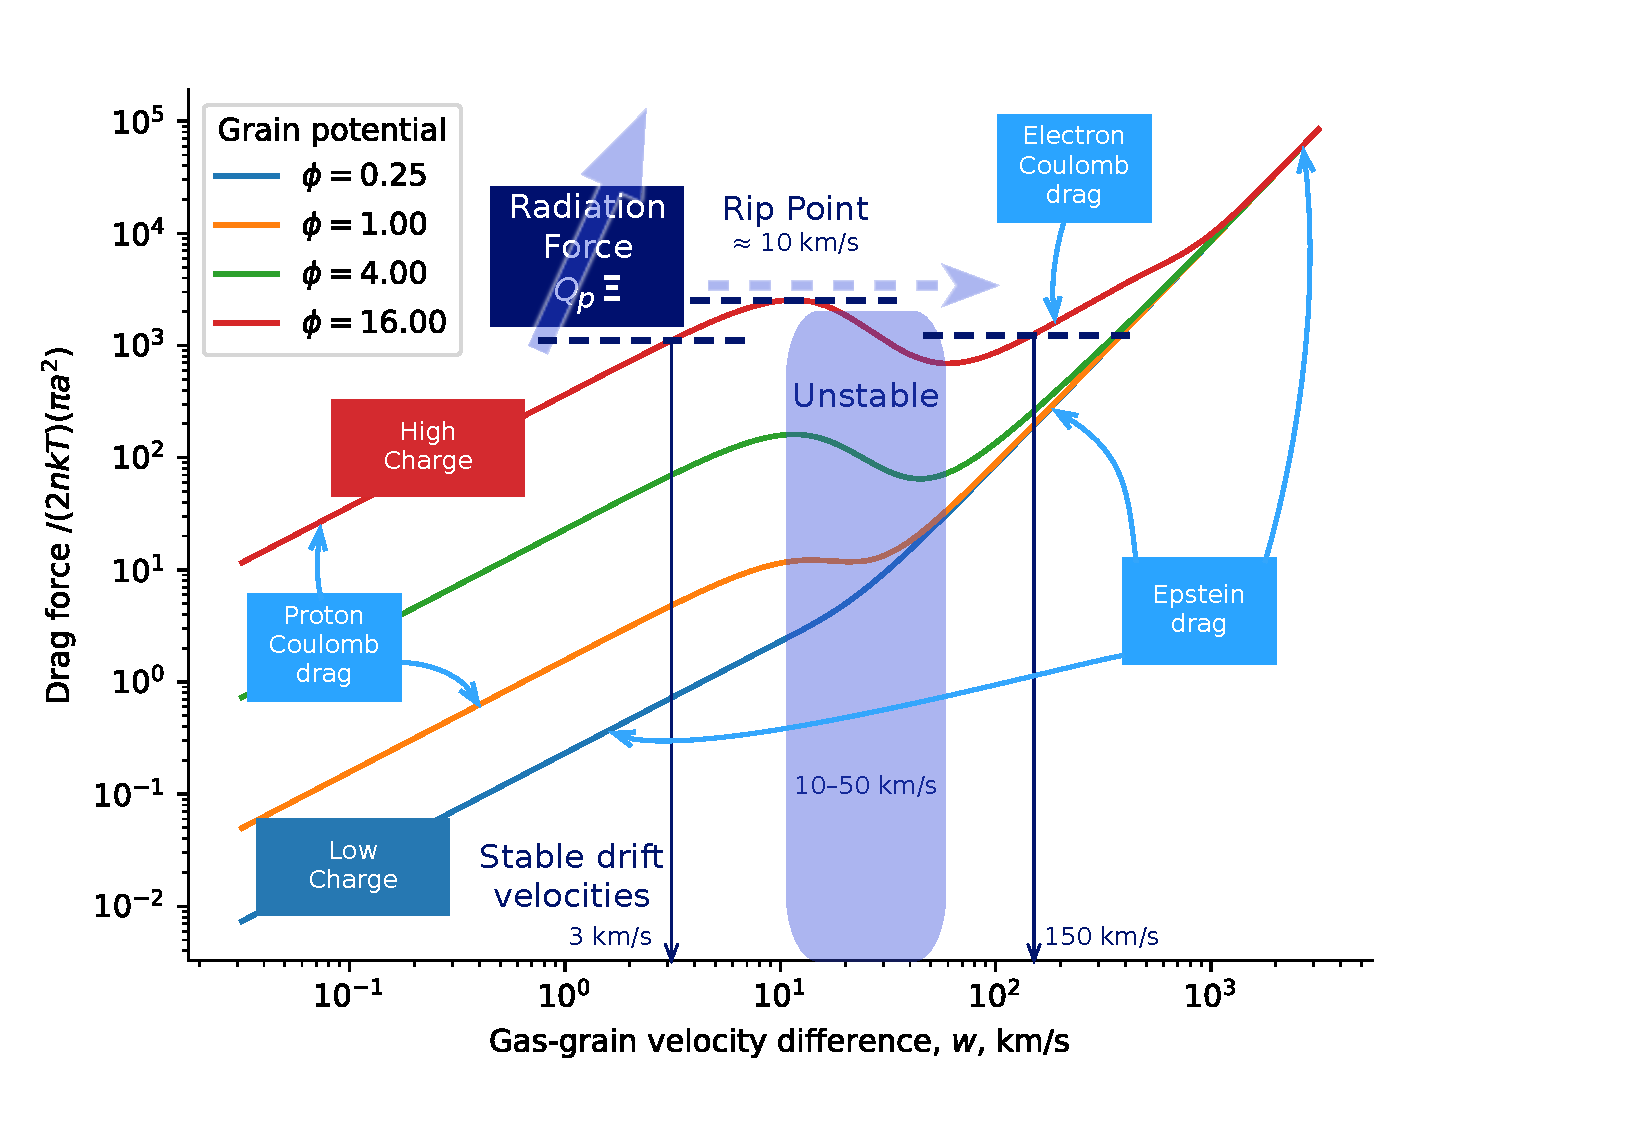
\includegraphics[width=\linewidth]{figs/gas-grain-drag-photoionized}
  \caption{Dimensionless drag force, \(f\drag / f_*\), as a function
    of gas--grain slip velocity, \(w\), for different values of the
    grain potential in thermal units, \(\phi\).  Contributions from
    proton and electron Coulomb (electrostatic) drag, as well as
    Epstein (solid-body) drag are indicated.  Examples of subsonic and
    highly supersonic stable drift velocities are shown (thin dark
    blue arrows), where the drag force is in equilibrium with the
    radiation force (thick dark blue dashed lines), while blue shading
    indicates the unstable, mildly supersonic velocity regime, where
    no stable drift equilibrium exists.  Inset graph shows \(\phi\) as a
    function of the radiation parameter,
    \(\Xi = P_{\mathrm{rad}} / P_{\mathrm{gas}}\) on a log--linear scale
    for a collection of Cloudy models (see
    Appendix~\ref{sec:cloudy-models-dust}).}
  \label{fig:gas-grain-drag-photoionized}
\end{figure*}


\begin{figure}
  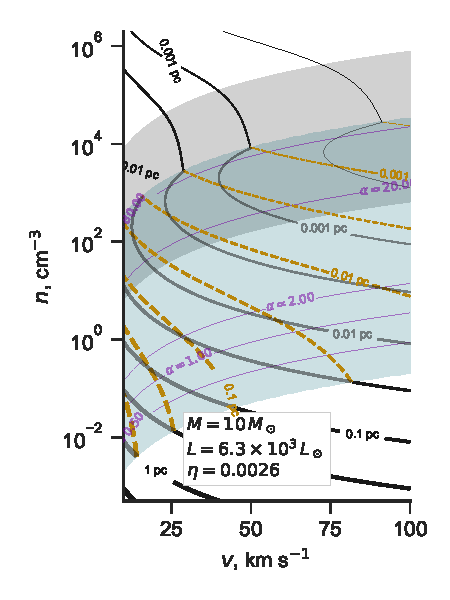
\includegraphics[width=\linewidth]{figs/decouple-v-n-plane}
  \caption{As Fig.~\ref{fig:zones-v-n-plane}(a), but accounting for
    gas-grain decoupling with constant efficiency \(\xi = 0.07\). }
  \label{fig:decouple-v-n-plane}
\end{figure}

\begin{figure}
  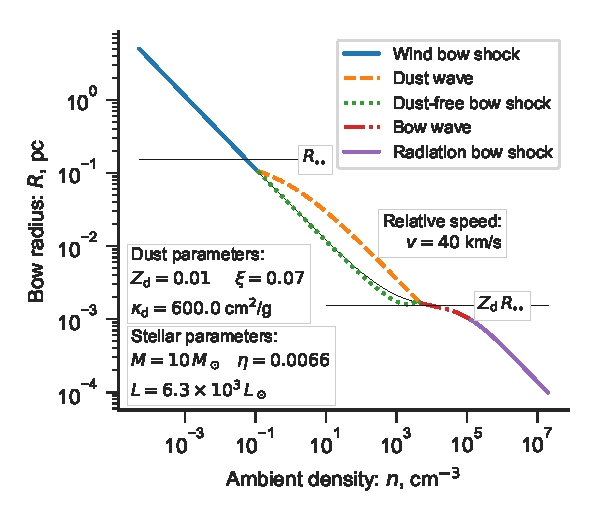
\includegraphics[width=\linewidth]{figs/decouple-v40-versus-n}
  \caption{Vertical cut through Fig.~\ref{fig:decouple-v-n-plane},
    showing bow radius and different regimes for a fixed inflow
    velocity of \SI{40}{km.s^{-1}}.}
  \label{fig:decouple-v40-versus-n}
\end{figure}


If the radiation field is sufficiently strong, then the collisional
coupling between grains and gas will break down.  In this section, we
calculate the regions of star+stream parameter space where this might
occur, leading to a separation of the bow into an outer dust wave and
an inner, dust-free bow shock.

\subsubsection{Drag force on grains}
\label{sec:drag-force-grains}

\begin{table}
  \centering
  \caption{Regimes of drag force as function of grain potential and slip speed}
  \label{tab:fdrag-regimes}
  \renewcommand\arraystretch{1.3}
  \resizebox{\linewidth}{!}{%
    \begin{tabular}{@{}r l l l@{}}
    \toprule
      & Regime & Approximate criteria & \(f\drag / f_*\) \\ \midrule
      I & Epstein subsonic & \(\phi^2 \ll 1\)
                             and \(w_{10} < 1\) & \(1.5\, w_{10}\) \\
      II & Epstein supersonic & \(w_{10} > 1\)
                                and \(w_{10} > 5\,\abs{\phi}\)& \( w_{10}^2\) \\
      III & Coulomb p\(^+\) subthermal & \(\phi^2 > 1\)
                                         and \(w_{10} < 1\) & \((1 + 20\, \phi^2)\,
                                                              w_{10}\) \\
    % & Coulomb p\(^+\) peak & \(\phi^2 > 1\)
    %                          and \(w_{10} \approx 1\) & \(1 + 10\, \phi^2\) \\
      IV & Coulomb p\(^+\) superthermal & \(\phi^2 > 1\)
                                          and \(1 < w_{10} < 5\) & \(w_{10}^2
                                                                   + 10\, \phi^2/w_{10}^2 \) \\
      V & Coulomb e\(^-\) subthermal & \(\phi^2 > 20\)
                                 and \(5 < w_{10} < 42\) & \(0.48\, \phi^2 \,
                                                           w_{10}\) \\
    \bottomrule
  \end{tabular}
  }
\end{table}

The drag force on a charged dust grain moving at a relative speed
\(w\) through a plasma has contributions from both direct collisions
and from electrostatic Coulomb interactions with ions and electrons.
We use the expressions in \citet{Draine:1979a}, equations~(4)--(6),
considering the contributions from protons, electrons, helium
ions,\footnote{Helium is assumed to be singly ionized, leading to only
  a small contribution to the drag force.  For much hotter stars, such
  as the central stars of planetary nebulae, helium may be doubly
  ionized, which leads to a fourfold increase in its Coulomb drag
  contribution, which is significant for \(w < \SI{5}{km.s^{-1}}\).} %
and metal ions.\footnote{%
  \label{fn:metal-drag}
  All metals are lumped together as a single species, assuming
  standard \hii{} region gas-phase abundances.  They are dominated by
  C and O, with minor contributions from N and Ne.  The total
  abundance is \num{8.5e-4} and the effective atomic weight is
  \num{15.3}.  All are assumed to be doubly ionized.  Their largest
  relative contribution to the drag force is for
  \(w < \SI{2}{km.s^{-1}}\), but is less than 1\% even there.} %
Results are shown in Figure~\ref{fig:drag-components}, where dashed lines correspond to direct solid body collisions and solid lines to electrostatic interactions.  The latter depend on the grain potential, which is described in dimensionless terms by \(\phi\), which is the electrostatic potential
energy of a unit charge at the surface of a grain of charge
\(z\grain\) and radius \(a\), in units of the characteristic thermal
energy of a gas particle:
\begin{equation}
  \label{eq:phi-potential}
  \phi = \frac{e^2 z\grain}{a kT} \ .
\end{equation}
The electrostatic contributions to \(f\drag\) are proportional to
\(\phi^2\) (results are shown for \(\abs{\phi} = 10\)), whereas the
solid-body contributions are independent of \(\phi\).  The drag force is
put in dimensionless units by dividing by a characteristic force:
\begin{equation}
  \label{eq:fstar}
  f_* = 2 n k T \cdot \pi a^2 \ , 
\end{equation}
which is approximately\footnote{%
  To simplify the exposition, the gas pressure in this section is
  calculated assuming a fully ionized, pure hydrogen plasma, yielding
  \(P\gas = 2 n k T\). For typical ISM abundances, the contribution of
  helium and its corresponding electrons yield a correction to this of
  order 5\%.  The required modifications when a cool star interacts
  with a predominantly neutral gas stream are discussed later.  } %
the ionized gas pressure multiplied by the grain geometric cross
section.

For grains with low electric charge, \(\phi^2 \ll 1\), the drag force is
dominated by direct collisions of protons with the grain (dashed red
line in Fig.~\ref{fig:drag-components}).  The gas collisional mean
free path is much larger than the grain size, so the drag is in the
Epstein regime \citep{Weidenschilling:1977b}.
% This is illustrated by
% the \(\phi = 0.25\) case (blue line) in
% Figure~\ref{fig:gas-grain-drag-photoionized}.
As the relative gas--grain slip speed, \(w\), increases, \(f\drag\)
first increases linearly with \(w\) reaching \(f\drag \approx f_*\) at
\(w = \sound \approx \SI{10}{km.s^{-1}}\), then transitions to a quadratic
increase in the supersonic regime.

As \(\abs{\phi}\) increases, long-range electrostatic interactions with
protons within the Debye radius (Coulomb drag) become increasingly
important at subsonic relative velocities, as shown by the solid lines
in Figure~\ref{fig:drag-components}).
% in
% Figure~\ref{fig:gas-grain-drag-photoionized} by the orange
% (\(\phi = 1\)), green (\(\phi = 4\)), and red (\(\phi = 16\)) lines.
However, the Coulomb drag has a peak when \(w\) is equal to the
thermal speed of the colliders, which is
\(\approx \SI{10}{km.s^{-1}}\) for protons, giving a maximum strength of
\begin{equation}
  \label{eq:fdrag-maximum}
  f_{\mathrm{max}} = 0.5\, (\ln\Lambda)\, \phi^2 f_* \approx 10\, \phi^2 f_* \ , 
\end{equation}
where \(\Lambda\) is the plasma parameter (number of particles within a
Debye volume), such that
\(\ln\Lambda = 23.267 + 1.5 \ln T_4 - 0.5 \ln n\).  At highly super-thermal
speeds, the Coulomb drag falls asymptotically as
\(f\drag \propto 1 / w^{2}\).  The thermal speed of electrons is higher than
that of the protons by a factor of \((m_p / m_e)^{1/2}\), so that the
electron Coulomb drag (solid light blue line) gives a second peak of
similar strength, but at \(w \approx \SI{430}{km.s^{-1}}\).  The behavior of
\(f\drag\) in all these different regimes is summarised in
Table~\ref{tab:fdrag-regimes}, in terms of \(\phi\) and
\(w_{10} = w / \SI{10}{km.s^{-1}}\).  This is further illustrated in
Figure~\ref{fig:drag-v-phi-plane}, where each of the drag regimes is
located on the \((w, \abs{\phi})\) plane.


% \begin{equation}
%   \label{eq:fdrag-regimes}
%   f\drag \approx
%   \begin{cases}
%     \text{Epstein subsonic (\(\phi^2 \ll 1\) and \(w_{10} < 1\)):}
%     & w_{10}\, f_* \\
%     \text{Epstein supersonic (\(\phi^2 \ll 1\) and \(w_{10} > 1\)):}
%     & w_{10}^2\, f_* \\
%     \text{Coulomb p\(^+\) subthermal (\(\phi^2 > 1\) and \(w_{10} < 1\)):}
%     & (1 + 20 \phi^2)\, w_{10}\, f_* \\
%     \text{Coulomb p\(^+\) peak (\(\phi^2 > 1\) and \(w_{10} \approx 1\)):}
%     & (1 + 10 \phi^2)\, f_* \\
%     \text{Coulomb p\(^+\) superthermal (\(\phi^2 > 1\) and \(1 < w_{10} < 5\)):}
%     & (w_{10}^2 + 10 \phi^2/w_{10}^2) \, f_* \\
%     \text{Coulomb e\(^-\) subthermal (\(\phi^2 > 20\) and \(5 < w_{10} < 42\)):}
%     & 0.48 \phi^2 \, w_{10}\, f_* \\
%   \end{cases}
% \end{equation}

% Or \Lambda = (4 pi / 3) n r_D^3?
% Where Debye length is r_D^2 = k T / 4 pi n e^2
% => \Lambda = n r_D (4 pi / 3) k T / 4 pi n e^2
% = k T r_D / 3 e^2
% This is 9 times less than the other expression
% Anyway, from kappa notes I have
% \ln\Lambda = 9.452 + 1.5 ln(T) - 0.5 ln(n)

% If I am going to use log10, then the coefficients get divided by
% ln(10) = 2.30258509299, and if we use T4, then we add 1.5 ln(1e4) =
% 13.815.  So we get 23.267 + 0.651 log10(T4) - 0.217 log10(n).  Nope,
% best with natural log

\subsubsection{Gas--grain separation: drift and rip}
\label{sec:gas-grain-separ}

In Appendix~\ref{sec:gas-free-bow} we calculate the behaviour of an
incoming stream of dust grains, subject only to the repulsive
radiation force from a star.  For an initial inward radial trajectory,
the dust grain motion is decelerated and turned around, reaching a
minimum radius \(R\starstar\), given by equation~\eqref{eq:dust-r0}.
This drag-free radiative turnaround radius, \(R\starstar\), is smaller
for higher initial inward velocities, but is independent of the
density of the incoming stream.  We are now in a position to see how
gas--grain drag will modify this picture.

From equations~\eqref{eq:dust-rad-force} and~\eqref{eq:fstar}, we can
write the radiation force acting on a grain as
\begin{equation}
  \label{eq:frad-Xi}
  f\rad = \Qp\, \Xi\, f_* \ ,
\end{equation}
where \(\Qp\) is the grain's radiation pressure efficiency (see
footnote~\ref{fn:Qp} in Appendix~\ref{sec:gas-free-bow}) and \(\Xi\) is
the local radiation parameter, defined as the ratio of direct stellar
radiation pressure to gas pressure:
\begin{equation}
  \label{eq:Xi-Prad-over-Pgas}
  \Xi \equiv \frac{P\rad}{P\gas} \approx \frac{L}{4 \pi R^2 c\, (2 n k T)} \ ,
\end{equation}
where the last expression corresponds to the optically thin limit.
The grain potential \(\phi\) is also primarily determined by \(\Xi\), as
shown in Appendix~\ref{sec:cloudy-models-dust} and the inset graph of
Figure~\ref{fig:gas-grain-drag-photoionized}, but with a slow
dependence, which can be approximated as
\begin{equation}
  \label{eq:phi-vs-Xi}
  \phi(\Xi) \approx 1.5 \bigl( 2.3 +  \ln \Xi \bigr) \ .
\end{equation}
There are also slight secondary dependencies on the grain composition and
stellar spectrum.  The relationship given in eq.~\eqref{eq:phi-vs-Xi}
is appropriate for graphite grains and for stellar effective
temperatures in the range \SIrange{20}{30}{kK}.  For hotter stars than
this, \(\phi\) should be multiplied by a further factor of \(1.5\), while
for silicate grains it should be divided by \(1.5\).

In the outer regions of the photoionized volume around an OB star,
close to the ionization front, the radiation parameter is low, with
typical value \(\Xi \sim 0.1\).  In this regime, the negative charge
current at the grain surface due to electron collisions is roughly in
balance with the positive current due to the ultraviolet photoelectric
effect \citep{Weingartner:2001b}, leading to a low grain potential,
\(\abs{\phi} < 1\), which may be positive or negative.  The low
\(\Xi\) means that the radiative force is also weak:
\(f\rad \sim 0.1 f_*\) from equation~\eqref{eq:frad-Xi} if
\(\Qp \sim 1\) at UV wavelengths, which is true for all but the smallest
grains.  Thus, from the equations for \(f\drag\) given in
Table~\ref{tab:fdrag-regimes}, the radiative force can be balanced by
Epstein drag if \(w_{10} \sim 0.1\), leading to a small equilibrium drift
velocity, \(w\drift < \SI{1}{km.s^{-1}}\), of the grains with respect
to the gas.  This drift is much smaller than the inward stream
velocities that we are considering
(\(v_\infty > \SI{10}{km.s^{-1}}\)), so the dust follows the gas stream at
a slightly reduced velocity (\(< 10\%\)), and (by mass conservation) a
slightly increased density.  Each grain exerts an exactly opposite
force to \(f\drag\) upon the gas, but since the dust-gas mass ratio,
\(Z\grain\), is small, this produces a negligible acceleration of the
gas.

\begin{table}
  \caption{Critical values of radiation parameter at the rip point: \(\Xi_\dag\)}
  \centering
  \begin{tabular*}{0.75\columnwidth}{l @{\quad\quad\quad\quad} S S} \toprule
    & \multicolumn{2}{c}{Grain composition} \\
    Spectrum & {Graphite} & {Silicate}
    \\ \midrule
    B star & 1000 +- 400 & 350 +- 150 \\
    O star & 3000 +- 500 & 2500 +- 500 \\
    \bottomrule
    \addlinespace
    \multicolumn{3}{@{}p{0.75\columnwidth}@{}}{
    Calculated from the Cloudy models shown in Figure~\ref{fig:drift-gn}. 
    Uncertainties represent variations with grain size and gas density. 
    See Appendix~\ref{sec:cloudy-models-dust} for further details.}
  \end{tabular*}
  \label{tab:Xi-rip}
\end{table}

As the dusty stream approaches the star, the radiation parameter
\(\Xi\) will increase, with a dependence of \(R^{-2}\) once the stream
is well inside the ionization front.  This increases \(f\rad\)
(eq.~[\ref{eq:frad-Xi}]), but also increases the grain potential,
\(\phi\) (eq.~[\ref{eq:phi-vs-Xi}]) due to the increasing dominance of
grain charging by photoelectric ejection.  Initially, this results in
a lowering of the equilibrium drift velocity to \(w_{10} \sim 0.01\) as
the Coulomb drag kicks in (see Appendix~\ref{sec:cloudy-models-dust}).
However, at smaller radii the slow logarithmic increase in
\(\phi(\Xi)\) means that the drift velocity must start increasing again to
accommodate the linear increase of \(f\rad(\Xi)\).  Eventually,
\(f\rad\) exceeds \(f_{\mathrm{max}}\), the maximum drag force that
proton Coulomb interactions can provide
(eq.~[\ref{eq:fdrag-maximum}]).  This occurs at a critical value of
the radiation parameter, which we denote the \textit{rip point}:
\(\Xi_\dag \sim 1000\).  The variations in \(\Xi_\dag\) with star and grain
parameters, which are of order \SI{+- 0.5}{dex}, are listed in
Table~\ref{tab:Xi-rip} and illustrated graphically in
Figure~\ref{fig:drift-gn}.

\subsubsection{Existence conditions for dust waves}
\label{sec:exist-cond-separ}

In order for a separate dust wave to exist, it is necessary for the
grains to decouple from the incoming gas stream before the stream hits
the hydrodynamic bow shock caused by the stellar wind.  The radius of
the rip point, \(R_\dag\), can be expressed in terms of \(R_*\), the
fiducial optically thick bow shock radius introduced in
\S~\ref{sec:strong-gas-grain}:
\begin{equation}
  \label{eq:Rdag-over-Rstar}
  R_\dag = \frac{v_\infty}{\sound}\, \Xi_\dag^{-1/2} R_* \approx v_{10}\, \Xi_\dag^{-1/2} R_* \ ,
\end{equation}
where we have made use of equations~\eqref{eq:Rstar}
and~\eqref{eq:Xi-Prad-over-Pgas}.  The wind bow shock radius is
\(R_0 = \eta^{1/2} R_*\) (eq.~[\ref{eq:x-cases}]), where \(\eta\) is the
wind momentum efficiency (eq.~[\ref{eq:wind-eta-typical}]).
Therefore, the condition \(R_\dag > R_0\) becomes
\begin{equation}
  \label{eq:dust-wave-velocity-condition}
  v_{10} > v_{10,\text{min}} = \bigl( \Xi_\dag \, \eta \bigr)^{1/2} \ . 
\end{equation}
For O stars, the wind efficiency is generally high (\(\eta > 0.1\)) and
\(\Xi_\dag > 2000\) (Tab.~\ref{tab:Xi-rip}), so that dust waves can only
exist when the stream velocity is very high
(\(v_\infty > \SI{150}{km.s^{-1}}\)).  For B~stars, in contrast, the wind
can be much weaker (\(\eta < 0.01\)) and \(\Xi_\dag\) is also smaller, so
that dust waves are permitted by this criterion for much lower stream
velocities: (\(v_\infty > \SI{30}{km.s^{-1}}\)).

\begin{figure*}
  \centering
  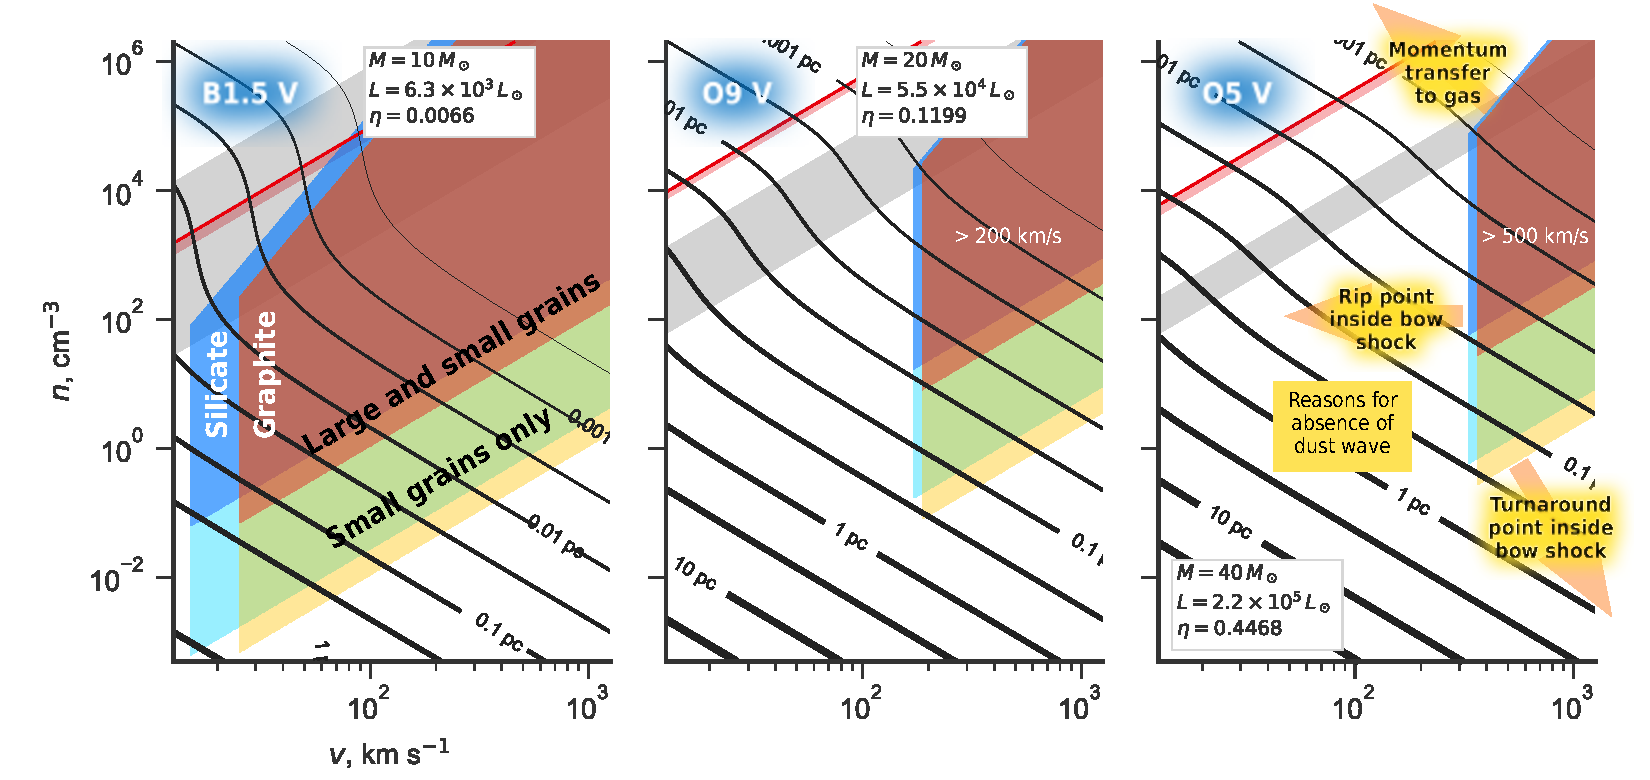
\includegraphics[width=\linewidth]{figs/existence-dust-wave}
  \caption{Regions of stream parameter space \((v, n)\) where dust
    waves may form around main-sequence OB stars of
    \SIlist{10;20;40}{M_\odot} (see Tab.~\ref{tab:stars}).  Figure is
    similar to Fig.~\ref{fig:zones-v-n-plane}, except that the
    velocity axis is logarithmic and extends out to
    \SI{1000}{km.s^{-1}}.  Overlapping colored shapes show parameters
    where dust waves may be allowed in the cases of large
    (\(a = \SI{0.2}{\um}\)) and small (\(a = \SI{0.02}{\um}\))
    graphite and silicate grains, as labeled in the left panel.  For
    \((v, n)\) outside of these shapes, dust waves cannot occur for
    the reasons indicated by labeled orange arrows in the center
    panel.  Labeled dashed lines in the right panel show the
    correspondence between the region boundaries and each dust wave
    existence condition given in
    equations~(\ref{eq:dust-wave-velocity-condition},
    \ref{eq:dust-wave-low-density-condition},
    \ref{eq:dust-wave-high-density-condition}). Heavy dashed lines in
    the left panel show where the rip point and the drag-free
    turnaround radius coincide.  For dust waves below these lines,
    drag forces are unimportant for the grains.  }
  \label{fig:existence-dust-wave}
\end{figure*}

However, there are other conditions that need to be satisfied in order
for the dust wave to exist.  For instance, the drag-free turnaround
radius must also be outside the bow shock: \(R\starstar > R_0\),
otherwise the radiation is incapable of repelling the grain
opportunely, even once it has decoupled from the gas.  From
equations~\eqref{eq:Rstar}, \eqref{eq:tau-star},
and~\eqref{eq:dust-r0} we find
\begin{equation}
  \label{eq:Rstarstar-over-Rstar}
  \frac{R\starstar}{R_*} = \frac{2 \sigma\grain \Qp \tau_*}{\kappa m\grain} \ , 
\end{equation}
so, if we define a single-grain opacity as
\(\kappa\grain = \sigma\grain \Qp / m\grain\), then this condition becomes
\begin{equation}
  \label{eq:dust-wave-low-density-condition}
  \tau_* >  \tau_{*,\text{min}} = 0.5\, \frac{\kappa}{\kappa\grain}\, \eta^{1/2} 
  % \frac{\kappa \eta^{1/2}}{2 \kappa\grain}
  \ . 
\end{equation}
The average value of the factor \(\kappa / \kappa\grain\) over the entire grain
population must be equal to the dust--gas mass ratio,
\(Z\grain \approx 0.01\), but the factor will vary between grains, according
to their size and composition.\footnote{%
  Remember that \(\kappa\) is the opacity per unit mass of gas, while
  \(\kappa\grain\) is the opacity per unit mass of a particular grain. In
  both cases, averaged over the stellar spectrum.} %
In particular, it will be relatively larger for the largest grains
(\(a \approx \SI{0.2}{\um}\)), which dominate the total dust mass, and
smaller for the smaller grains (\(a \approx \SI{0.02}{\um}\)), which
dominate the UV opacity.  Given the dependence of \(\tau_*\) on the
stream parameters (eq.~[\ref{eq:taustar-typical}]), for a given
stellar luminosity this condition corresponds to a minimum value for
\(n / v_\infty^2\).

A third condition comes from requiring \(R_\dag > R_0\) in the radiation
bow wave regime (see \S~\ref{sec:three-bow-regimes}), where
\(R_0 \approx 2 \tau_* R_*\).  This yields
\begin{equation}
  \label{eq:dust-wave-high-density-condition}
  \tau_* < \tau_{*,\text{max}} = 0.5\, v_{10}\, \Xi_\dag^{-1/2} \ , 
\end{equation}
which, for a given stellar luminosity, corresponds to a maximum value
for \(n / v_\infty^4\).  Thus, for a given stream velocity that satisfies
equation~\eqref{eq:dust-wave-velocity-condition},
equations~(\ref{eq:dust-wave-low-density-condition},
\ref{eq:dust-wave-high-density-condition}) determine respectively the
minimum and maximum stream density for which a dust wave can exist.

Further restrictions on the existence of dust waves arise when the
effects of magnetic fields are considered, as will be discussed in
\S~\ref{sec:magn-effects-grain} below.

\subsubsection{Grain trajectories along the symmetry axis}
\label{sec:grain-traj-along}

What happens to the dust grain following this catastrophic breakdown
of gas--grain coupling depends on the relation between the rip point
radius, \(R_\dag\), and the drag-free radiative turnaround radius,
\(R\starstar\).  If \(R_\dag > R\starstar\), then the grain's inertia
will still carry it in as far as \(R\starstar\) and the initial
trajectory will be almost identical to that described in
Appendix~\ref{sec:gas-free-bow} for the drag-free case. However, after
being turned around by the radiation field and pushed out past
\(R_\dag\) again, the grain will \emph{recouple} to the gas and be
dragged back for a second approach.\footnote{If the initial impact
  parameter of the trajectory is not strictly \(b = 0\), then the
  resultant lateral component of \(f\rad\) will mean that \(b\) will
  be much increased for the second approach.} %
From equations~(\ref{eq:Rdag-over-Rstar},
\ref{eq:Rstarstar-over-Rstar},
\ref{eq:dust-wave-high-density-condition}), the condition
\(R_\dag > R\starstar\) corresponds to
\(\tau_* < (\kappa/\kappa\grain) \tau_{*,\text{max}}\), which is indicated by dashed
lines in the left panel of Figure~\ref{fig:existence-dust-wave}.  If,
on the other hand, \(R_\dag < R\starstar\), then the tail wind provided
by the gas carries the grain closer to the star than its inertia would
naturally take it.  When the grain finally decouples at \(R_\dag\) it
experiences a much higher unbalanced \(f\rad\), which can initially
accelerate it to outward velocities significantly higher than the
inflow velocity if \(R_\dag \ll R\starstar\).

\begin{figure*}
  \centering
  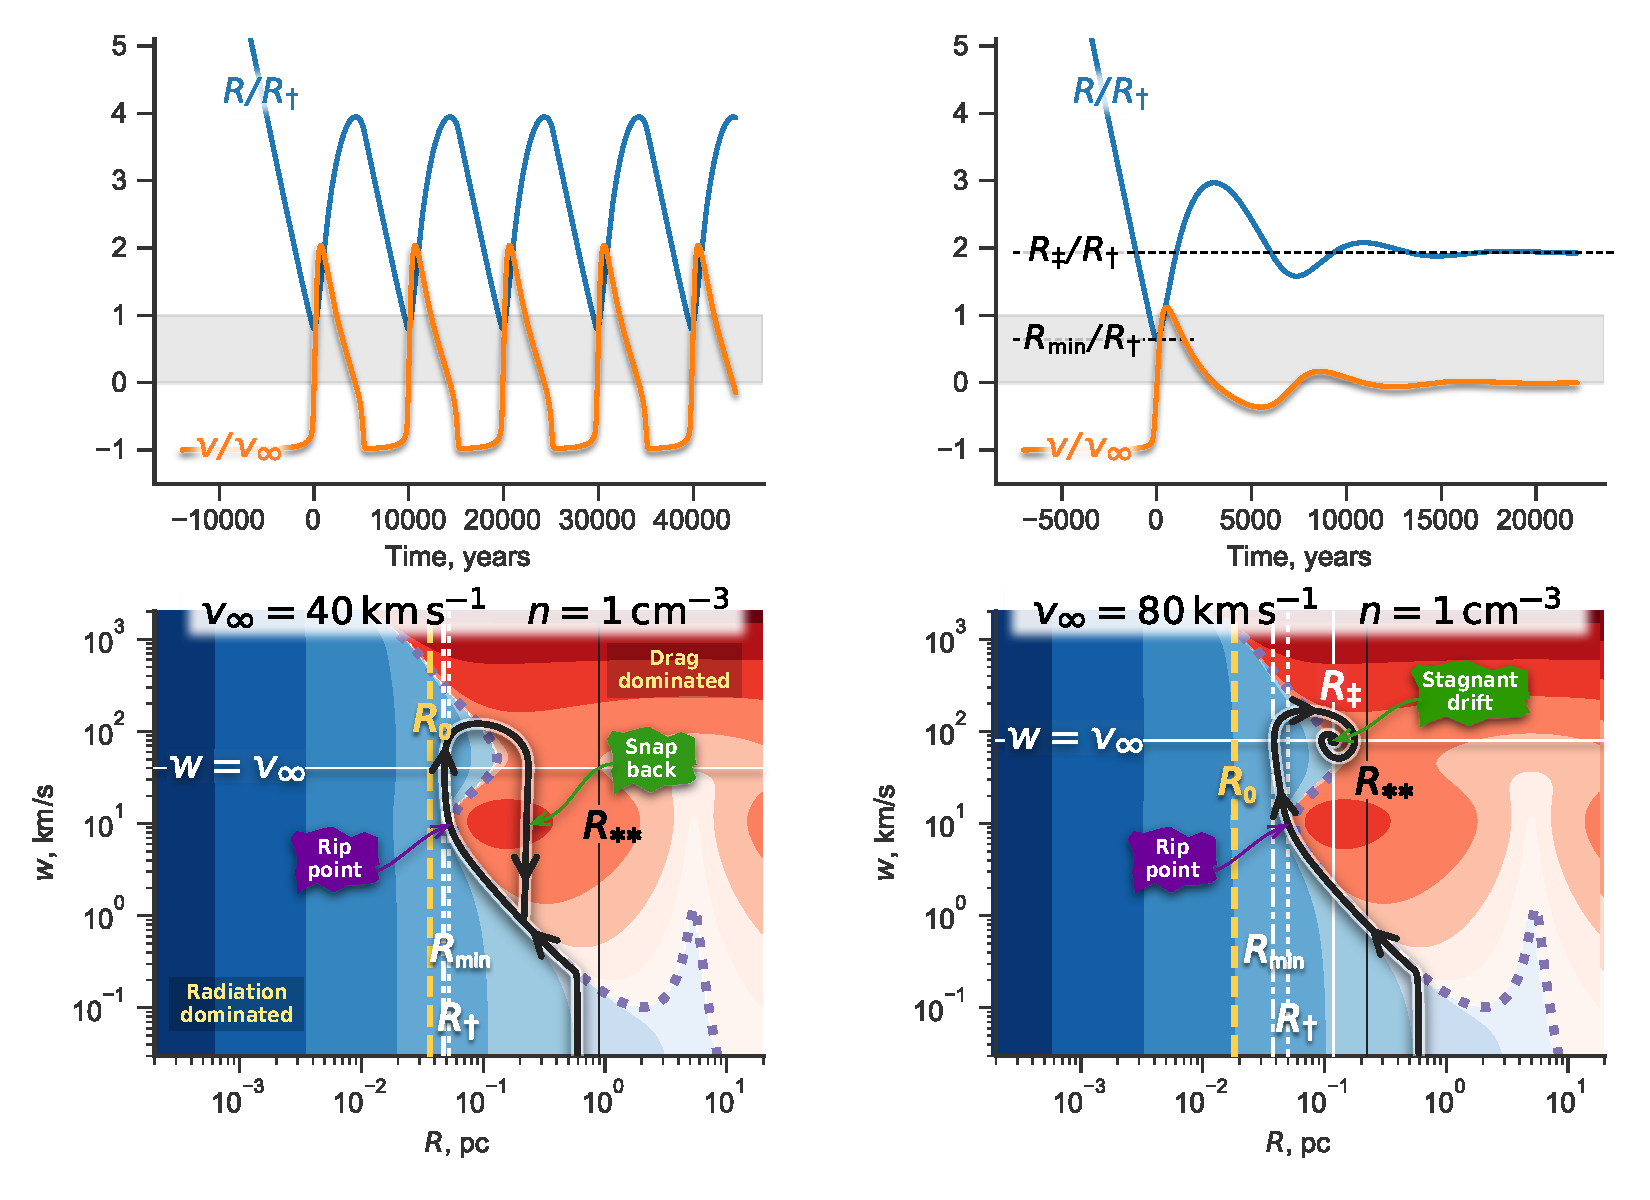
\includegraphics[width=\linewidth]{figs/dust-wave-phase-trajectories-annotate}
  \caption{Trajectories of small graphite grains
    (\(a = \SI{0.02}{\um}\)) at impact parameter \(b = 0\) for two
    example cases (see yellow ``+'' symbols in left panel of
    Fig.~\ref{fig:existence-dust-wave}), which differ only in the
    stream velocity: \(v = \SI{40}{km.s^{-1}}\) (left panels) and
    \SI{80}{km.s^{-1}} (right panels).  In both cases, the stream
    density is \(n = \SI{1}{cm^{-3}}\) and the central star is a
    \SI{10}{M_\odot} main-sequence B star (see Tab.~\ref{tab:stars}).
    Upper panels show the evolution of grain radius, \(R\) (blue
    curve, normalized by the rip point radius, \(R_\dag\)), and grain
    velocity, \(v\) (orange curve, normalized by the gas stream
    velocity).  The origin of the time axis is set to the moment of
    closest approach of the grain to the star: \(R = \Rmin\).  Lower
    panels show the trajectories in phase space: position versus
    gas--grain relative slip velocity (\(w = \abs{v - v_\infty}\)).  Filled
    contours show the net force on the grain: \(f\rad - f\drag\), with
    positive values in blue and negative values in red.  The heavy
    dotted line shows where there is no net force: \(f\rad = f\drag\).
    The grain trajectory (thick, solid black line with arrows)
    initially follows this line, but departs from it after the rip
    point. In the left panel, the grain enters a limit cycle between
    decoupling (rip) and re-coupling (snap back).  In the right panel,
    the grain spirals in on the stagnant drift point.  See text for
    further details.}
    \label{fig:phase-space-trajectories}
\end{figure*}

The post-decoupling behavior of the grain depends on the sign of
\(d f\drag / d w\) when \(w = \abs{v_\infty}\).  If this derivative is
positive, as is the case in drag regimes~II and V (see
Tab.~\ref{tab:fdrag-regimes} and Fig.~\ref{fig:drag-v-phi-plane}),
then the grain can reach a stable equilibrium drift at rest with
respect to the star\footnote{%
  Again, this is only strictly true when the impact parameter is zero.
  However, as we show below, it is a reasonable approximation over a
  range of impact parameters in the case where the angle between the
  magnetic field direction and the stream velocity is not too
  large.} %
at a point \(R_\ddag\), which we call the \textit{stagnant drift
  radius}. If the stream velocity is not excessively high
(\(v_\infty < \SI{150}{km.s^{-1}}\) when \(\phi = 4\), or
\(< \SI{300}{km.s^{-1}}\) when \(\phi = 16\)), then the equilibrium
\(f\rad\) is less than the value at the rip point, requiring a lower
value of the radiation parameter: \(\Xi_\ddag < \Xi_\dag\).  The resultant
stagnant drift radius is therefore outside the rip point:
\(R_\ddag > R_\dag\).

On the other hand, if \(d f\drag / d w < 0\) when
\(w = \abs{v_\infty}\), then the equilibrium is unstable and no stagnant
drift is possible.  This occurs for drag regime~IV, which applies when
\(\phi > 1\) and
\(\SI{10}{km.s^{-1}} < v_\infty < \SI{50}{km.s^{-1}}\).  There is also a
second unstable regime (partially visible in the upper-right corner of
Fig.~\ref{fig:drag-v-phi-plane}), which is related to the thermal peak
in the electron Coulomb drag when \(\phi > 30\) and
\(\SI{400}{km.s^{-1}} < v_\infty < \SI{2000}{km.s^{-1}}\), but this is not
relevant to bow shocks around OB~stars.\footnote{%
  It may apply in other contexts, such as outflows from AGN, since
  detailed modeling of grain charging around quasars
  \citep{Weingartner:2006a} implies that grain potentials as high as
  \(\phi \sim 100\) can be achieved.} %

An examples of each of these two behaviors is illustrated in
Figure~\ref{fig:phase-space-trajectories}.  The left panels show the
case where \(v_\infty = \SI{40}{km.s^{-1}}\), which is in the unstable
regime, resulting in periodic ``limit-cycle'' behavior (the parameters
of this model correspond to the yellow ``plus'' symbol labeled ``40''
in the left panel of Fig.~\ref{fig:existence-dust-wave}).  During the
grain's first approach, it starts to follow a phase trajectory (lower
left panel) along the \(f\rad - f\drag = 0\) contour, corresponding to
equilibrium drift, in which the grain begins to move a few
\si{km.s^{-1}} slower than the gas stream.  Then, when it reaches the
rip point (\(R = R_\dag\), \(w \approx \SI{10}{km.s^{-1}}\)) it suddenly
experiences a large unbalanced outward radiation force (blue region of
phase space in Fig.~\ref{fig:phase-space-trajectories}). The grain's
inward momentum carries it to the point \(\Rmin \approx 0.85 R_\dag\), before
it is expelled at roughly twice the inflow speed.  However, after
moving outward, it finds itself in a drag-dominated region of phase
space (red in the figure), and so recouples to the inflowing gas
stream.  The recoupling initiates gradually, as the grain's outward
motion is slowed and it begins to move inward again, but is completed
suddenly once \(w\) again falls below \SI{10}{km.s^{-1}}, in what we
term \textit{snap back}. The net result is that the grain has returned
to exactly the same phase track that it started in on, and so repeats
the cycle indefinitely.

The right panels of Figure~\ref{fig:phase-space-trajectories} show the
case where the stream velocity is doubled to
\(v_\infty = \SI{80}{km.s^{-1}}\), but all other parameters remain the
same.  At this velocity, the equilibrium drift is stable and so the
grain can achieve a stagnant drift solution, where it is stationary
with respect to the star.  The trajectory during the first approach is
similar to the previous case, except that the overshoot of the rip
point is greater, so that \(\Rmin \approx 0.65 R_\dag\) in this case.  This is
a consequence of the fact that the rip point is closer to the
drag-free turnaround radius (\(R_\dag / R\star\star\) is not so small as in the
lower velocity case), so that the grain inertia is relatively more
important.  A second consequence is that the speed of the initial
expulsion is not so large, being only a little higher than the inflow
velocity (but opposite to it).  The qualitative difference between the
two cases emerges after the first recoupling: instead of the snap back
and endless limit cycle, the grain oscillates about the stagnant drift
radius with ever decreasing amplitude, so that it has come almost to
rest after a few oscillation periods.


\subsubsection{Magnetic effects on grain trajectories }
\label{sec:magn-effects-grain}



\section{The case of inside-out bows}
\label{sec:case-inside-out}

So far, we have considered the case where the inner source dominates
the radiation, while dust is present only in the outer stream, which
applies to hot stars interacting with the ISM.  However, in the case
of cool stars, the inner wind will also be dusty.  Examples are the
red supergiant (RSG) phase of high-mass evolution, or the asymptotic
giant branch (AGB) stage of low/intermediate-mass evolution.  In both
these cases, it is still the inner source that provides the radiation
field.  However, not all winds are radiatively driven and in those
cases it is conceivable that it is the outer source that dominates the
radiation field.  An example is the case of photoevaporating
protoplanetary disks (proplyds) in the Orion Nebula and other \hii{}
regions \citep{ODell:1994a}.  In the proplyds, the inner wind is a
thermally driven photoevaporation flow \citep{HA:1998, Henney:1999a},
while the outer stream is the stellar wind from an O~star
\citep{Garcia-Arredondo:2001a}.


%%% Local Variables:
%%% mode: latex
%%% TeX-master: "dusty-bow-wave"
%%% End:

\section{Discussion}
\label{sec:summary-discussion}

Are there any objects that might not be bow shocks?

Progression in density:
\begin{gather*}
  \text{Increasing density} \longrightarrow \\
  \text{WBS} \to \text{WBS} + \text{IDW} \to \text{WBS} + \text{DDW} \to \text{(RBW)} \to \text{RBS}
\end{gather*}

Chief diagnostic for radiation supported bows (RBW or RBS cases) is
infrared luminosity of bow.  Favored by high densities.

Dust waves favored by high velocities and intermediate densities.

\newcommand\IR{\ensuremath{_{\text{IR}}}}

In order to provide an empirical anchor to our theoretical
calculations, we now consider how the parameters of our models might
be determined from observations.  The parameter space diagrams, such
as Figures~\ref{fig:zones-v-n-plane} and
\ref{fig:existence-dust-wave}, are not particularly useful in this
regard, since in many cases the ambient density and relative stellar
velocity are not directly measured.  Instead, we aim to construct
diagnostics based on the most common observations, which are of the
infrared dust emission.

A fundamental parameter is the optical depth, \(\tau\), of the bow shell
to UV radiation, which determines what fraction of the stellar photon
momentum is available to support the shell (see
\S~\ref{sec:three-bow-regimes}).  But the same photons also heat the
dust grains in the bow, which re-radiate that energy predominantly at
mid-infrared wavelengths (roughly \SIrange{10}{100}{\um}) with
luminosity \(L\IR\).  Assuming that Ly\(\alpha\) and mechanical heating of
the dust shell is negligible and that the emitting shell subtends a
solid angle \(\Omega\), as seen from the star, then the optical depth can
be estimated as
\begin{equation}
  \label{eq:tau-empirical}
  \tau = -\ln \left( 1 - \frac{4\pi}{\Omega} \frac{L\IR}{L_*} \right)
  \approx \frac{2 L\IR}{L_*} \ ,
\end{equation}
where the last approximate equality holds if \(\tau \ll 1\) and the shell
emission covers one hemisphere.\footnote{%
  The \(\tau\) of \S~\ref{sec:three-bow-regimes} is not exactly the same
  as the \(\tau\) of equation~\eqref{eq:tau-empirical}, but is larger by
  a factor of \(1 + \varpi (1 - g)/(1 - \varpi)\), where \(\varpi\) is
  the grain albedo and \(g\) the scattering asymmetry (see
  App.~\ref{sec:gas-free-bow}).} %

A second important parameter is the thermal plus magnetic pressure in
the shocked shell, which is doubly useful since in a steady state it
is equal to \emph{both} the internal supporting pressure (wind ram
pressure plus absorbed stellar radiation) \emph{and} the external
confining pressure (ram pressure of ambient stream).  The shell pressure is
not given directly by the observations, but can be determined as
follows:
\begin{enumerate}[1.]
\item The shell mass column (\si{g.cm^{-2}}) can be estimated from the
  optical depth by assuming an effective UV opacity: \(\Sigma\shell = \tau / \kappa\)
\item The shell density (\si{g.cm^{-3}}) can be found from the mass
  column if the shell thickness is known:
  \(\rho\shell = \Sigma / h\shell\).  In the absence of other information, a
  fixed fraction of the shell radius can be used.  In particular, we
  normalize by a typical value of one~quarter\footnote{%
    This corresponds to a Mach number \(\M_0 = \surd 3\) if the stream
    shock is radiative, or \(\M_0 \gg 1\) if non-radiative (see
    \S~\ref{sec:radi-cool-lengths}).  Further discussion is given in
    Appendix~\ref{app:bow-shock-data}} %
  the star--apex distance:
  \(h_{1/4} = h\shell / (0.25 R_0)\).
\item Finally, the pressure (\si{dyne.cm^{-2}}) follows by assuming
  values for the sound speed and Alfvén speed:
  \(P\shell = \rho\shell (\sound^2 + \frac12 v\alfven^2) \).
\end{enumerate}
It is natural to normalize this pressure to the stellar radiation
pressure at the shell, so we define a shell momentum efficiency
\newcommand\pc{\ensuremath{_{\text{pc}}}}
\begin{equation}
  \label{eq:eta-shell}
  \eta\shell \equiv \frac{P\shell}{P\rad}
  = \frac{4\pi R_0^2\, (\sound^2 + \frac12 v\alfven^2)\, \tau}{L_*\, \kappa\, h\shell}
  \approx 245 \frac{R\pc \, T_4 \, \tau}{L_4 \, \kappa_{600} \, h_{1/4}} \ , 
\end{equation}
where in the last step we have assumed ionized gas with negligible
magnetic support (\(v\alfven \ll \sound\)) and written the stellar
luminosity and shell parameters in terms of typical values, as in
\S~\ref{sec:depend-stell-type}.  Note that the shell momentum
efficiency is simply the reciprocal of the radiation parameter of
equation~\eqref{eq:Xi-Prad-over-Pgas}:
\(\eta\shell = \Xi\shell^{-1}\), which provides yet a third use for
\(\eta\shell\), since \(\Xi\) is paramount in determining whether the
grains and gas remain well-coupled (see
\S~\ref{sec:exist-cond-separ}).

\begin{table}
  \centering
  \caption[Observational]{Key observational parameters for star/bow systems}
  \label{tab:observations}
  \begin{tabular}{l S S S}
    \toprule
    Star & {\(L_* / \si{L_\odot}\)} & {\(L_{\text{IR}} / \si{L_\odot}\)} & {\(R_0 / \si{pc}\)} \\
    \midrule
    \thD & 2.95e4 & 620 & 0.003 \\
    LP~Ori & 1600 & 240 & 0.01 \\
    \(\sigma\)~Ori & 6e4 & 15 & 0.12 \\[\smallskipamount]
    K18 Sources & \numrange{1.4e4}{8.7e5} & \numrange{8}{2800} & \numrange{0.02}{1.35} \\
    \bottomrule
  \end{tabular}
\end{table}


\begin{figure*}
  \centering
  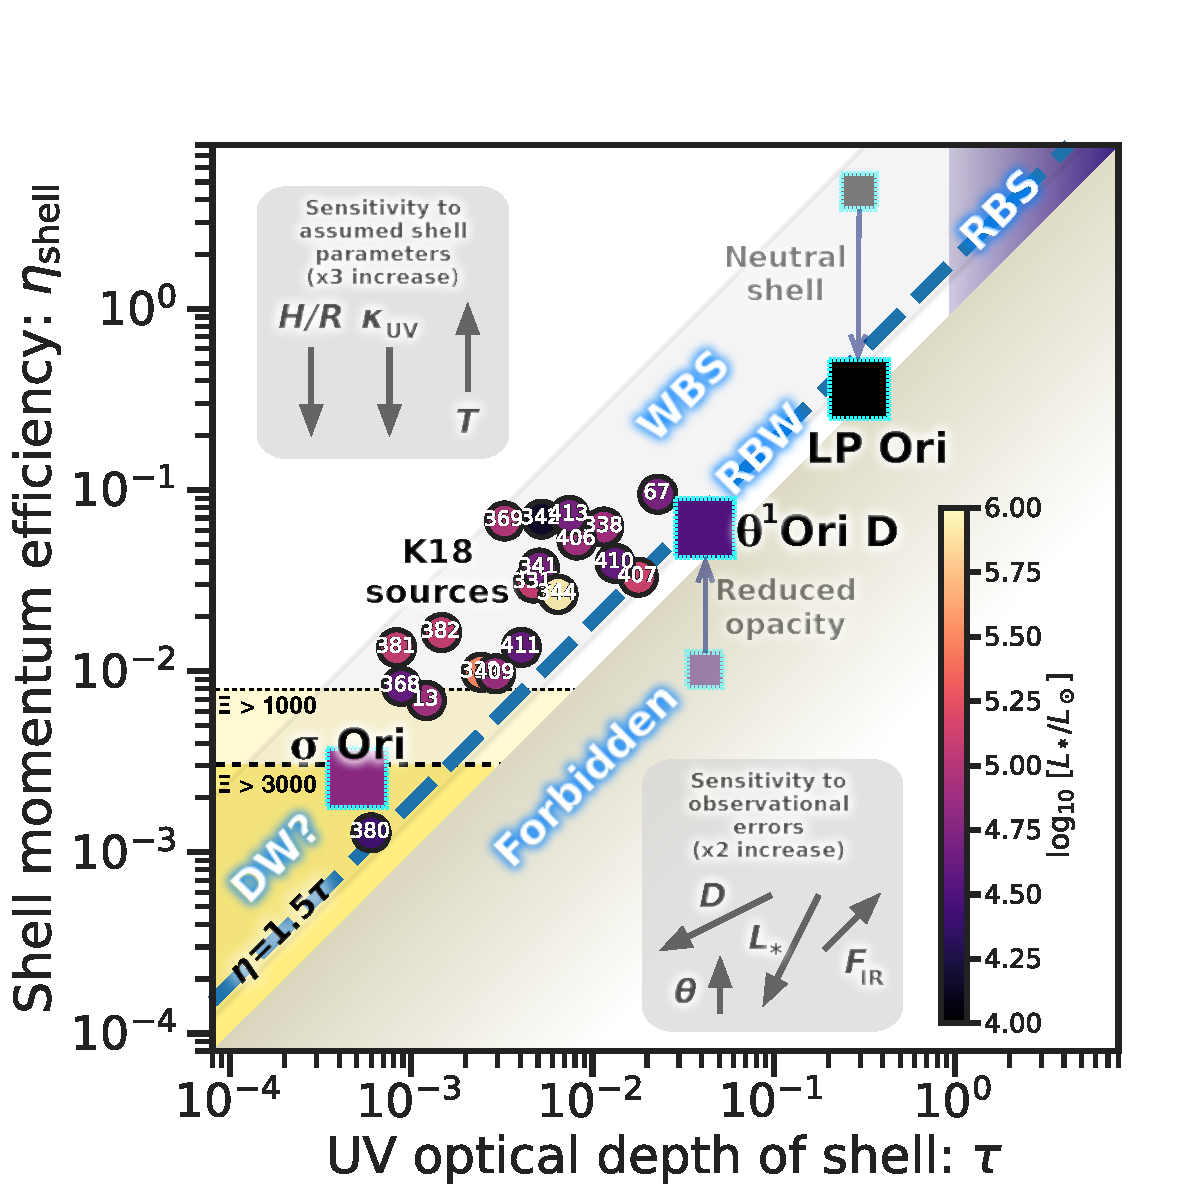
\includegraphics[width=\linewidth]{figs/All-sources-eta-tau}
  \caption[Observational diagnostic diagram]{Observational diagnostic
    diagram for bow shocks.  The shell optical depth \(\tau\) (\(x\)
    axis) and momentum efficiency \(\eta\shell\) (\(y\) axis) can be
    estimated from observations of the bolometric stellar luminosity,
    infrared shell luminosity, and shell radius, as described in the
    text.  Results are shown for the 20 sources (circle symbols) from
    \citet{Kobulnicky:2018a} plus three further sources (square
    symbols), where we have obtained the measurements ourselves (see
    Tab.~\ref{tab:observations}).  The color of each symbol indicates
    the stellar luminosity (dark to light) as indicated by the scale
    bar. The shell pressure is determined assuming a gas temperature
    \(T = \SI{e4}{K}\), an absorption opacity
    \(\kappa = \SI{600}{cm^2.g^{-1}}\), and a thickness-to-radius ratio
    \(H/R = 0.25\).  The sensitivity of the results to a
    factor-of-three change in each parameter is shown in the upper
    inset box.  Exceptions are the two Orion Nebula sources, \thD{}
    and LP~Ori, where the small dim squares show the results of
    assuming the standard shell parameters, while the large squares
    show the results of modifications according to the peculiar
    circumstances of each object, as described in the text.  The lower
    inset box shows the sensitivity of the results to a factor-of-two
    uncertainty in each observed quantity: distance to source \(D\);
    stellar luminosity \(L_*\), shell infrared flux \(F\IR\); shell
    angular size \(\theta\).  Lines and shading indicate different
    theoretical bow regimes (see \S\S~\ref{sec:strong-gas-grain} and
    \ref{sec:imperf-coupl-betw}).  The dashed blue diagonal line
    corresponds to radiation-supported bows, while the upper left
    region corresponds to wind-supported bows.  The upper right corner
    (purple) corresponds to optically thick bow shocks, while the
    lower left corner (yellow) is the region where grain--gas
    separation \textit{may} occur, leading to a potential dust wave.
    However, the existence of a dust wave in this region is not
    automatic, since it only includes one of the four necessary
    conditions (\S~\ref{sec:exist-cond-separ} and
    \S~\ref{sec:grain-traj-with}). The lower-right region is strictly
    forbidden, except in case of violation of the assumption that dust
    heating be dominated by stellar radiation. }
  \label{fig:All-sources-eta-tau}
\end{figure*}



Mass loss rates - starting from \citet{Kobulnicky:2010a}

Different scenarios for producing velocities: dynamic ejection from
young clusters \citep{Hoogerwerf:2001a, Oh:2016c} produce high
velocities, dissolution of binary systems following core-collapse SN
\citep{Renzo:2018a} tend to produce lower velocities for the unbound
MS companion (walkaways, slower than 30 km/s).  Also, champagne flows
have low velocities.

How different regions of the \(\Pi\)--\(\Lambda\) plane are populated.
Bottom-right quadrant hard to get to (except for standing wave
oscillations), but may be due to finite shell thickness, which (for
low Mach number) will be more apparent in the wings, which might
decrease \(\Lambda\) more than \(\Pi\).  Fact that thin-shell solutions should
trace the contact discontinuity, but in some cases it may be only the
inner or the outer shell that is visible.

Justification for standing waves: Fig.~3 of \citet{Meyer:2016a} shows
a time sequence of thin-shell instability, which looks a bit like a
standing wave. But much larger amplitude than we are considering.

Deviations from axisymmetry as an alternative to oscillations. 


\subsection{The case of inside-out bows}
\label{sec:case-inside-out}

So far, we have considered the case where the inner source dominates
the radiation, while dust is present only in the outer stream, which
applies to hot stars interacting with the ISM.  However, in the case
of cool stars, the inner wind will also be dusty.  Examples are the
red supergiant (RSG) phase of high-mass evolution, or the asymptotic
giant branch (AGB) stage of low/intermediate-mass evolution.  In both
these cases, it is still the inner source that provides the radiation
field.  However, not all winds are radiatively driven and in those
cases it is conceivable that it is the outer source that dominates the
radiation field.  An example is the case of photoevaporating
protoplanetary disks (proplyds) in the Orion Nebula and other \hii{}
regions \citep{ODell:1994a}.  In the proplyds, the inner wind is a
thermally driven photoevaporation flow \citep{HA:1998, Henney:1999a},
while the outer stream is the stellar wind from an O~star
\citep{Garcia-Arredondo:2001a}.


\section{Summary and conclusions}
\label{sec:conclusions}



%%% Local Variables:
%%% mode: latex
%%% TeX-master: "dusty-bow-wave"
%%% End:

\bibliographystyle{mnras}
\bibliography{bowshocks-biblio}
\appendix

\section{Grain charging and gas--grain coupling around OB stars}
\label{sec:cloudy-models-dust}

We calculate models of the physical properties of dust grains using
the plasma physics code Cloudy \citep{Ferland:2013a, Ferland:2017a},
which self-consistently solves the multi-frequency radiative transfer
together with thermal, ionization, and excitation balance of all
plasma constituents.  Cloudy incorporates grain charging as described
in \citet{Baldwin:1991a} and \citet{van-Hoof:2004a} with photoelectric
emission theory from \citet{Weingartner:2001b, Weingartner:2006a}.  We
use the default ``ISM'' dust mixture included in Cloudy, which
comprises ten size bins each for spherical silicate and graphite
grains in the range \num{0.005} to \SI{0.25}{\um}, and which is
designed to reproduce the average Galactic extinction curve
\citep{Weingartner:2001a, Abel:2008a}.  The optical properties of each
grain species are calculated using Mie theory \citep{Bohren:1983a},
assuming solid spheres.  The resultant wavelength-dependent extinction
properties of the mixture are summarised in
Figure~\ref{fig:cloudy-ism-dust-opacity}.

\begin{figure}
  \centering
  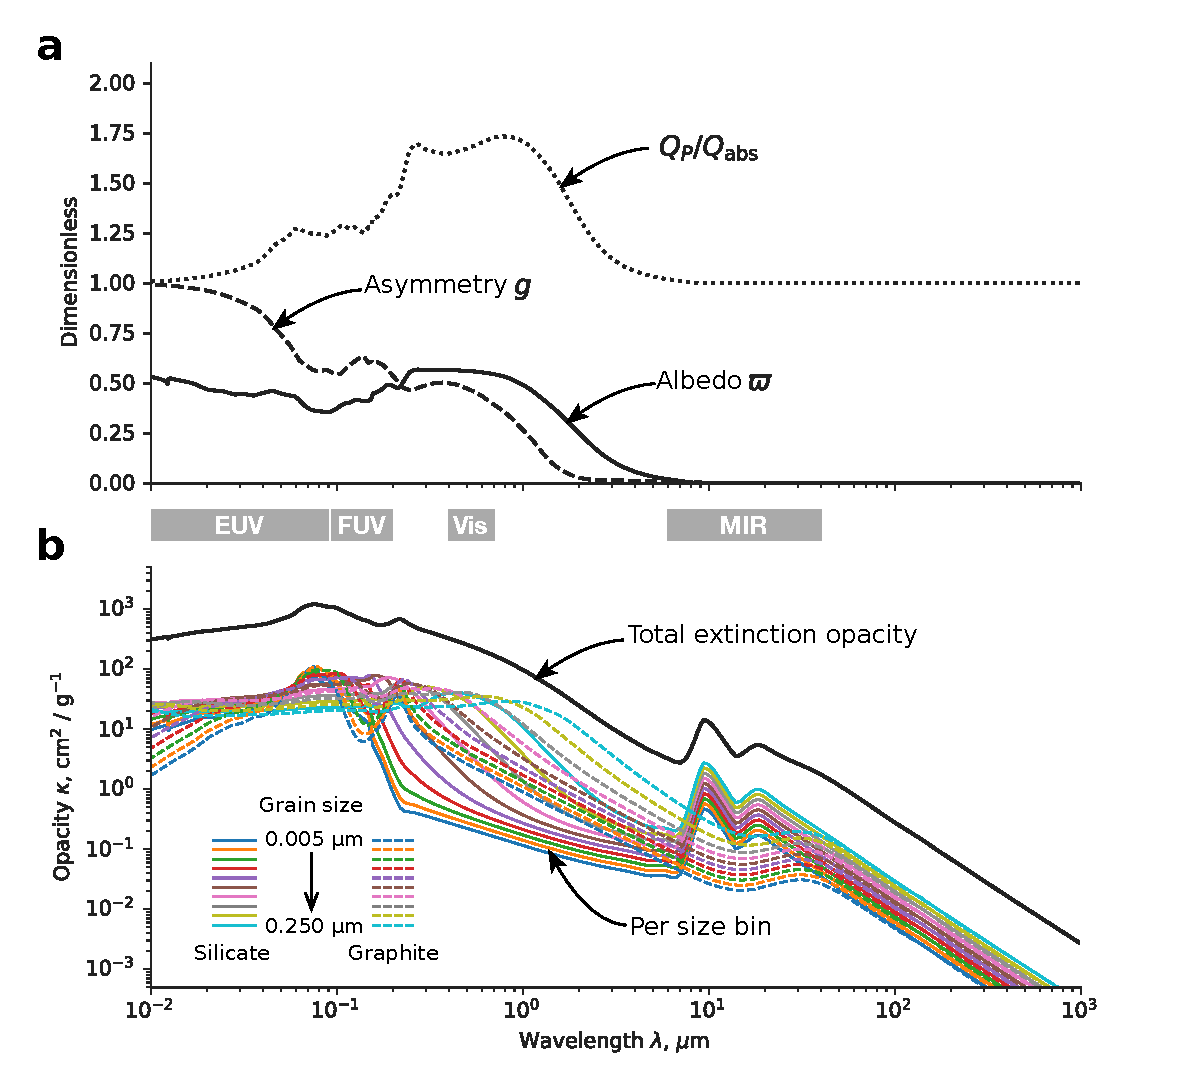
\includegraphics[width=\linewidth]{figs/cloudy-ism-dust-opacity}
  \caption{Extinction properties of Cloudy's standard ``ISM'' dust
    mixture. %
    (a)~Wavelength dependence of mean values over the entire mixture
    of three dimensionless quantities related to scattering: albedo,
    \(\varpi\) (solid line); scattering asymmetry,
    \(g = \langle \cos\theta \rangle\) (dashed line); ratio of radiation pressure
    efficiency to absorption efficiency, \(Q_P / Q_{\text{abs}}\)
    (dotted line).
    %
    (b)~Wavelength dependence of mass opacity (cross section per unit
    mass of gas) for the whole mixture (heavy black line) and broken
    down by size bin and grain composition (colored lines, see key). }
  \label{fig:cloudy-ism-dust-opacity}
\end{figure}

To ascertain the expected variation in grain properties in the
circumstellar environs of luminous stars, we calculate a series of
spherically symmetric, steady-state, constant density Cloudy simulations,
illuminated by the stars listed in Table~\ref{tab:stars}, with stellar
spectra taken from the OSTAR2002 and BSTAR2006 grids, calculated with
the TLUSTY model atmosphere code \citep{Lanz:2003a, Lanz:2007a}.
Simulations are run for hydrogen densities of
\numlist{1;10;100;e3;e4} \si{cm^{-3}} and assuming standard \hii{} region
gas phase abundances.  The calculation is stopped when the ionization
front is reached and the inner radius is chosen to be roughly 1\% of this. 



\begin{figure*}
  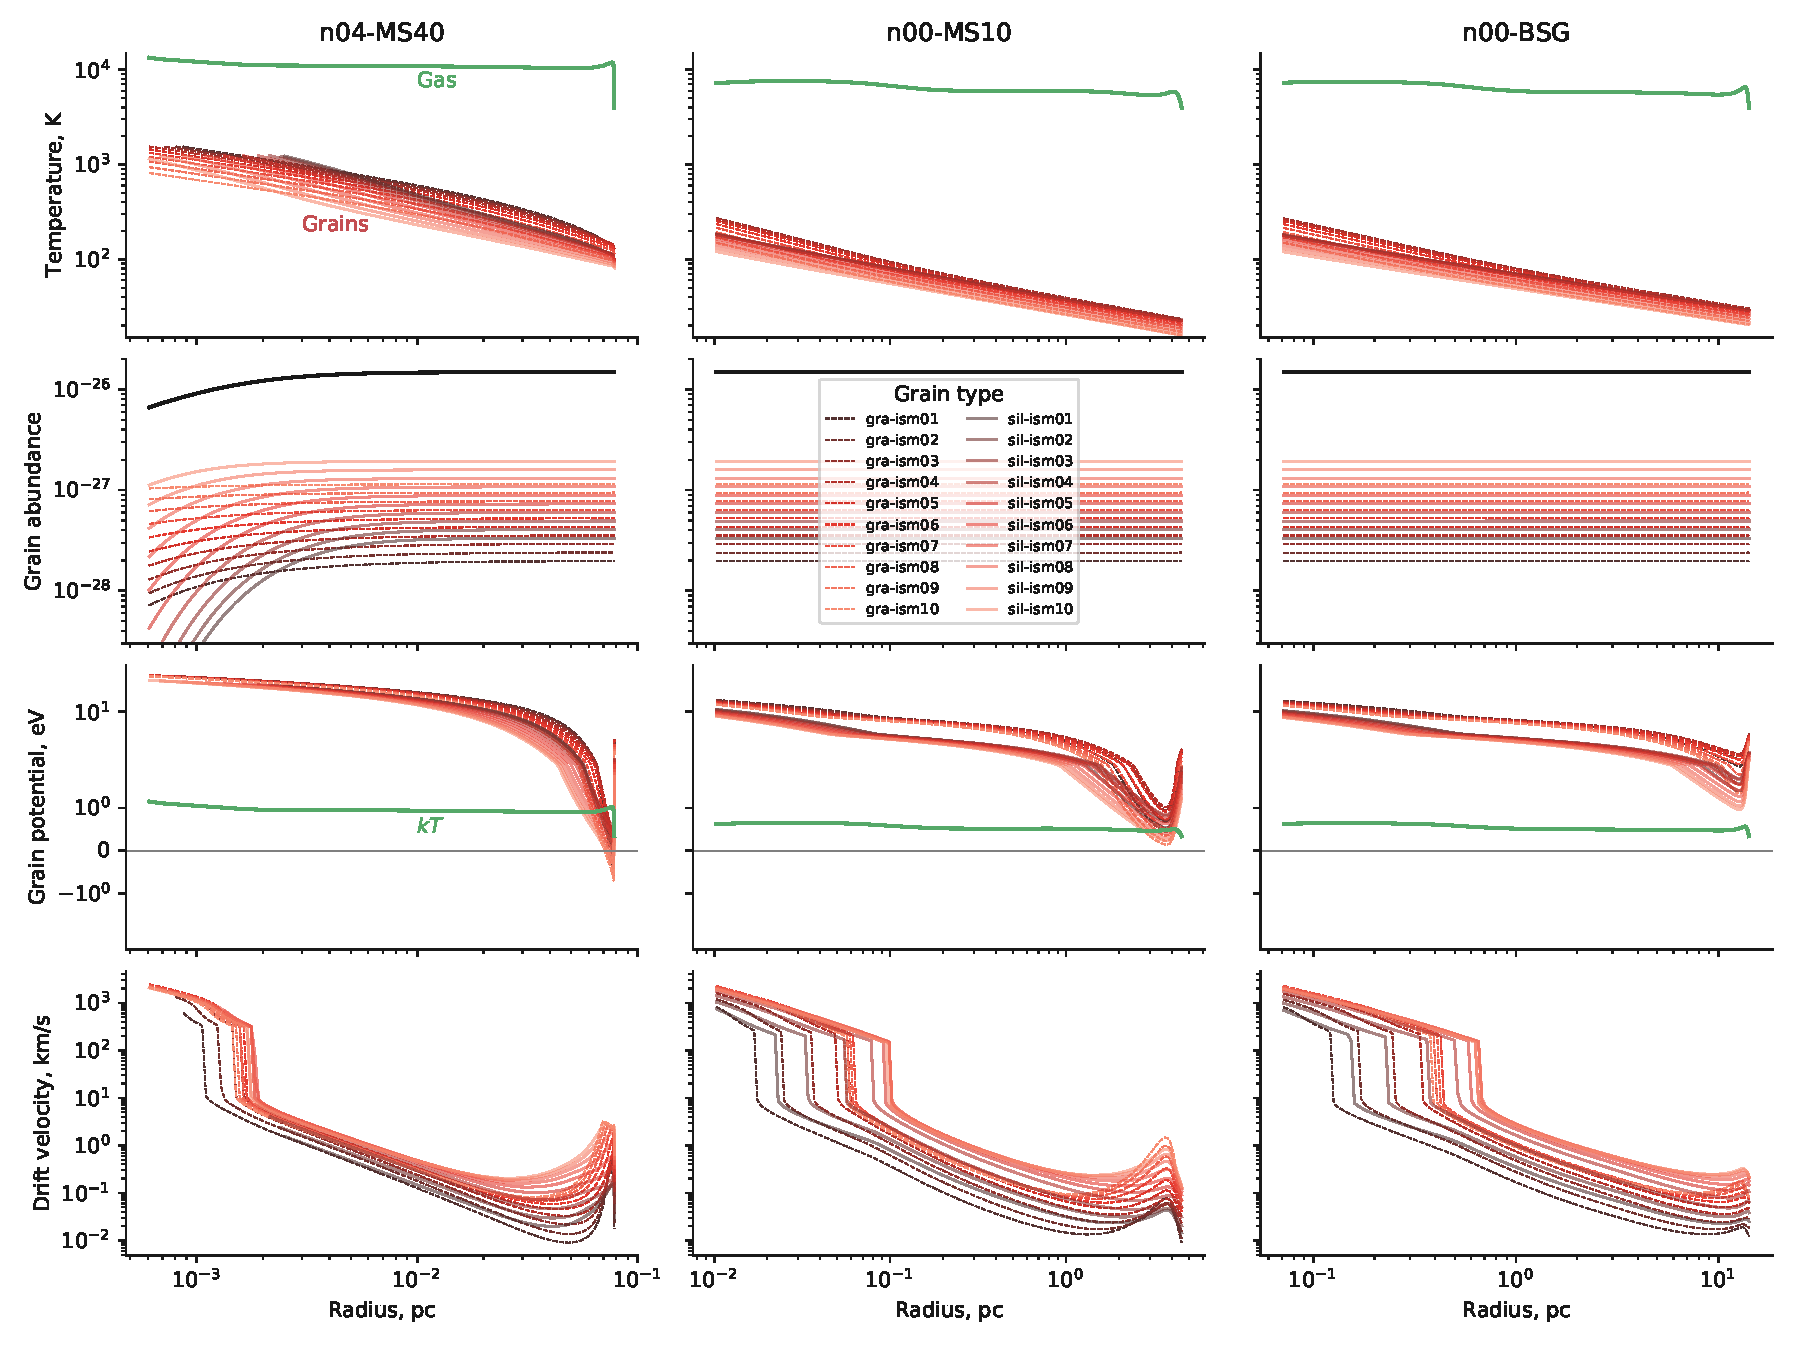
\includegraphics[width=\linewidth]{figs/multi-dustprops}
  \caption{Dust properties as a function of radius from star for three
    selected Cloudy simulations. (a)~\SI{40}{M_\odot} main-sequence star in
    medium of density \SI{e4}{cm^{-3}}. (b)~\SI{10}{M_\odot} main-sequence
    star in medium of density \SI{1}{cm^{-3}}. (c)~Blue supergiant
    star in medium of density \SI{1}{cm^{-3}}}.
  \label{fig:multi-dustprops}
\end{figure*}
Figure~\ref{fig:multi-dustprops} shows resultant radial profiles of
dust properties for representative simulations: grain temperature, grain
abundance, grain potential, and grain drift velocity.  Line types
correspond to the different size bins of graphite and silicate grains,
as indicated in the key from smallest to largest. The left hand panels
show results for a high-density (\(n = \SI{e4}{cm^{-3}}\)), compact
(\(R \approx \SI{0.1}{pc}\)) region around an early O~star, where the grain
temperature is very high, especially for the smaller silicate grains,
and sublimation significantly reduces the grain abundance in the inner
regions.  The remaining columns show low-density
(\(n = \SI{1}{cm^{-3}}\)), extended (\(R \sim \SI{10}{pc}\)) regions
around main-sequence and supergiant B-type stars, in which the grain
temperatures are much lower, ranging from \SIrange{20}{50}{K} in the
outer parts up to \SIrange{100}{200}{K} in the inner parts.

 
\begin{figure*}
  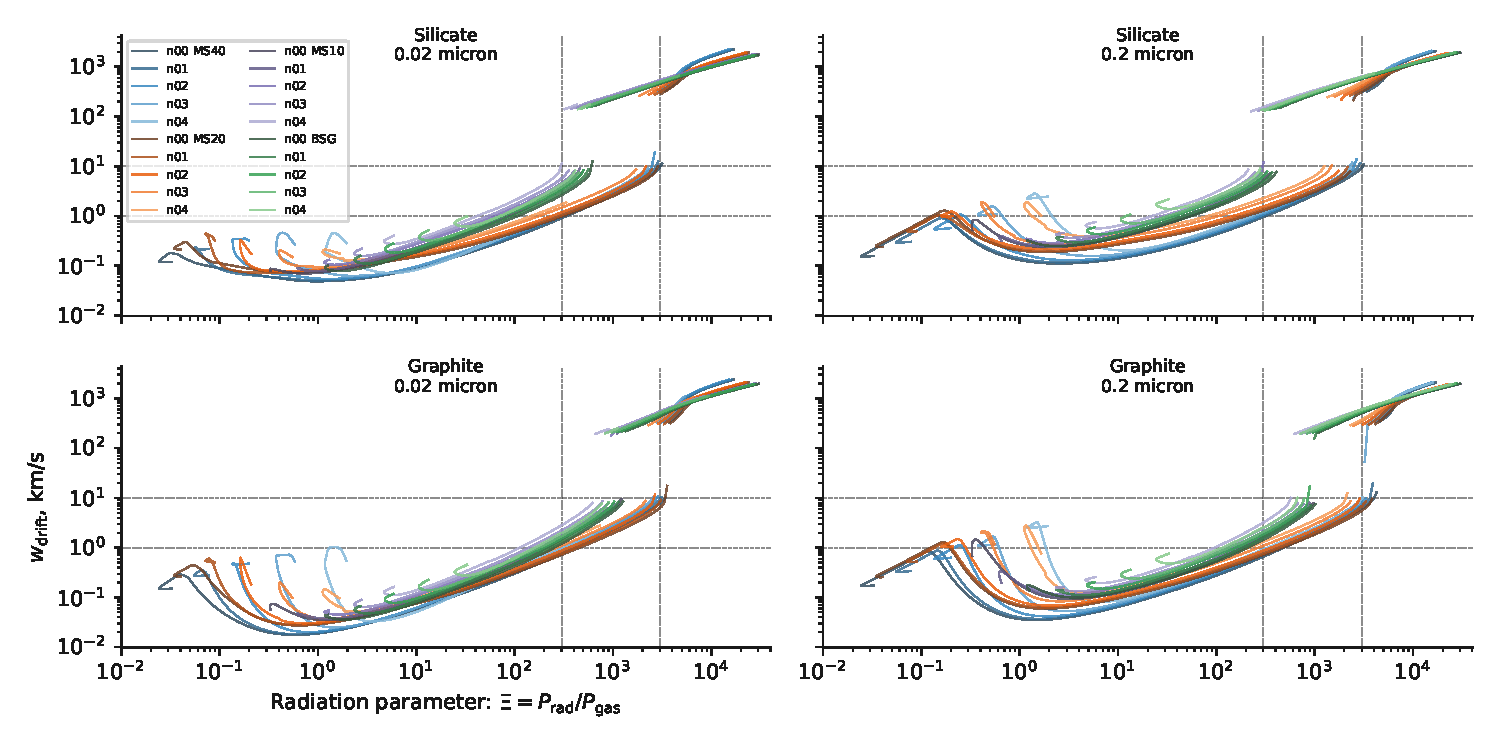
\includegraphics[width=\linewidth]{figs/drift-pratio-4panel}
  \caption{Drift velocity \(w\drift\) versus radiation parameter
    \(\Xi\). Each line represents a simulation with ambient density and
    stellar type as indicated in the key.  Results are shown for
    graphite and silicate grains of two different sizes.  The rip
    point, which corresponds to gas--grain decoupling, is the
    discontinuity in the curves at
    \(w\drift \approx \SI{10}{km.s^{-1}}\), indicated by the upper
    horizontal dashed line.  The vertical dashed lines show the narrow
    range of radiation parameter, \(\Xi = 1000 \pm \SI{0.5}{dex}\), that
    encompasses the rip point for all simulations. }
  \label{fig:drift-gn}
\end{figure*}

Unlike the strong differences in thermal properties, the radial
dependence of grain electrostatic potential (third row in
Fig.~\ref{fig:multi-dustprops}) is qualitatively similar for all the
simulations.  The grains are predominantly positively charged, with high
potentials (\(> 10\) times the thermal energy of gas particles) close
to the star due to the strong EUV and FUV photo-ejection.  The
potential falls to much lower values in the outer ionized region, as
the EUV flux falls off, and then climbs again at the ionization front
due to the fall in electron density, while the FUV photo-ejection
persists well into the neutral region.  There are small differences
between the simulations due to the increasing relative importance of the
EUV radiation for hotter stars, which leads to a deeper dip in the
potential just inside the ionization front for the \SI{40}{M_\odot} case,
even reaching negative values for some grain species.

Equilibrium drift velocity for each grain species is calculated in the
Cloudy simulations using the same theory \citep{Draine:1979a} as
outlined in \S~\ref{sec:drag-force-grains}.  The way that this is
implemented by default in Cloudy means that if the only solution at
the inner radius is a superthermal one, then the superthermal solution
branch (upper right corner of
Fig.~\ref{fig:gas-grain-drag-photoionized}) is followed as far as
possible through the outer spatial zones.  We have modified the code
so as to instead always prefer the slower subthermal branch whenever
multiple solutions are available.  This makes the most sense in our
context, where the grains are moving towards the star and so the
radiative force is gradually increasing from an initial low value.
Example results are shown in the bottom row of
Figure~\ref{fig:multi-dustprops} and again they are qualitatively
similar for all the simulations.  Close to the star, the radiation
force is higher than the upper limit on the Coulomb drag force
(eq.~[\ref{eq:fdrag-maximum}]), so that the equilibrium drift velocity
is exceedingly high.\footnote{Note that such high drift velocities are
  much higher than any realistic true relative velocity between grains
  and gas, since they are based on the assumption that the radiation
  force remains constant while the grain is accelerated, which is not
  the case near the rip point.  Instead, they are simply an indication
  that the gas and grains have completely decoupled.}.  As the radial
distance from the star increases, the radiation field is increasingly
diluted but the grain potential falls only slowly, so eventually one
reaches a point where an equilibrium between Coulomb drag and
radiation force can be established, which corresponds to a
discontinuity in the drift velocity.  This is the \textit{rip point}
discussed in \S~\ref{sec:gas-grain-separ}.  The drift velocity carries
on falling towards the outside of the \hii{} region, but then
increases again just inside the ionization front due to the drop in
grain potential there.

Both the charge balance and the force balance are essentially due to
competition between the photons and the charged particles that
interact with the grain.  It is therefore reasonable to surmise that
the gas--grain decoupling that occurs at the rip point might be
determined principally by the ratio of photons to gas particles.  We
test this hypothesis in Figure~\ref{fig:drift-gn}, where we
characterize the photon-gas ratio by a dimensionless radiation
parameter, \(\Xi\), equal to the radiation pressure divided by the gas
pressure.  Results are shown for four different grain types and for
all combinations of stellar parameters and ambient densities for which
we have run simulations.  It can be seen that the rip point does indeed
always occur at a similar value of \(\Xi \sim 1000\) for all simulations, albeit
with some variation according to the spectral type of the star and the
grain composition, as given in Table~\ref{tab:Xi-rip}.  The gas
density and grain size have very little influence on this critical
value \(\Xi_\dag\), with the only exception being the very smallest grains
(\(a < \SI{0.006}{\um}\), not illustrated), which show
\(\Xi_\dag \approx \num{e4}\), but such grains are only minor contributors to the
UV opacity (\(< 10\%\) in EUV and \(< 1\%\) in FUV, see
Fig.~\ref{fig:cloudy-ism-dust-opacity}).

\begin{figure}
  \centering
  \includegraphics[width=\linewidth]{figs/phi-versus-xi-annotate}
  \caption{Grain potential in thermal units (linear scale) versus
    radiation parameter (logarithmic scale). All densities and stellar
    types are shown, with line colors as in Fig.~\ref{fig:drift-gn}.
    Solid lines show silicate grains and dashed lines show graphite
    grains.  Line width increases with grain size (to reduce clutter,
    only every second size bin is shown).  The solid and dashed lines
    show the logarithmic fits discussed in the text.}
  \label{fig:phi-vs-Xi}
\end{figure}
Finally, Figure~\ref{fig:phi-vs-Xi} shows the slow dependence of grain
potential on radiation parameter for all the simulations on a linear
versus logarithmic scale.  The logarithmic fit of
equation~\eqref{eq:phi-vs-Xi}, most appropriate for carbon grains
around cooler stars, is shown by the solid line.  The dashed lines
show the modifications for silicate grains and for hotter stars (see
\S~\ref{sec:gas-grain-separ}).  Further details of the Cloudy dust
models are discussed in Appendix~\ref{sec:grain-temp-emiss}.

\section{Grain temperature and mid-infrared emissivity}
\label{sec:grain-temp-emiss}


\begin{figure}
  \centering
  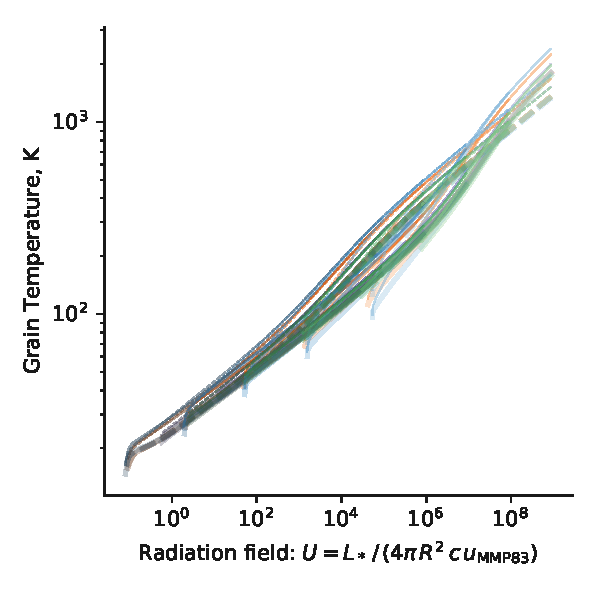
\includegraphics[width=\linewidth]{figs/grain-T-vs-U}
  \caption{Grain temperature versus radiation field mean intensity,
    \(U\), in units of the interstellar radiation field in the solar
    neighborhood.  Line types and colors are as in
    Fig.~\ref{fig:phi-vs-Xi} and correspond to a variety of stellar
    spectral shapes, gas densities, and grain species.}
  \label{fig:grain-T-vs-U}
\end{figure}

Figure~\ref{fig:grain-T-vs-U} shows equilibrium grain temperatures for
the Cloudy models discussed in Appendix~\ref{sec:cloudy-models-dust}
as a function of the nominal energy density of the radiation field,
\(U = u / u\mmp \), where \(u = L / 4 \pi R^2 c\) and \(u\mmp\) is the
energy density of the interstellar radiation field for
\(\lambda < \SI{8}{\um}\) in the solar neighborhood
\citep{Mathis:1983a}:
\begin{equation}
  \label{eq:u-mmp83}
  u\mmp\,c = \SI{0.0217}{erg.s^{-1}.cm^{-2}} \ .
\end{equation}
The tight relationship seen in figure~\ref{fig:grain-T-vs-U} between
\(T\) and \(U\) is evidence for the dominance of stellar radiative
heating (see \S~\ref{sec:unimp-other-heat} below), while the variation
about the mean relation is mainly due to differences in grain size and
composition, with smaller grains and graphite grains being relatively
hotter.  The downward hooks seen on the left end of each simulation's
individual curve are due to the fact that our calculation of \(U\)
does not account for internal absorption, which starts to become
important near the ionization front.

\begin{figure}
  \centering
  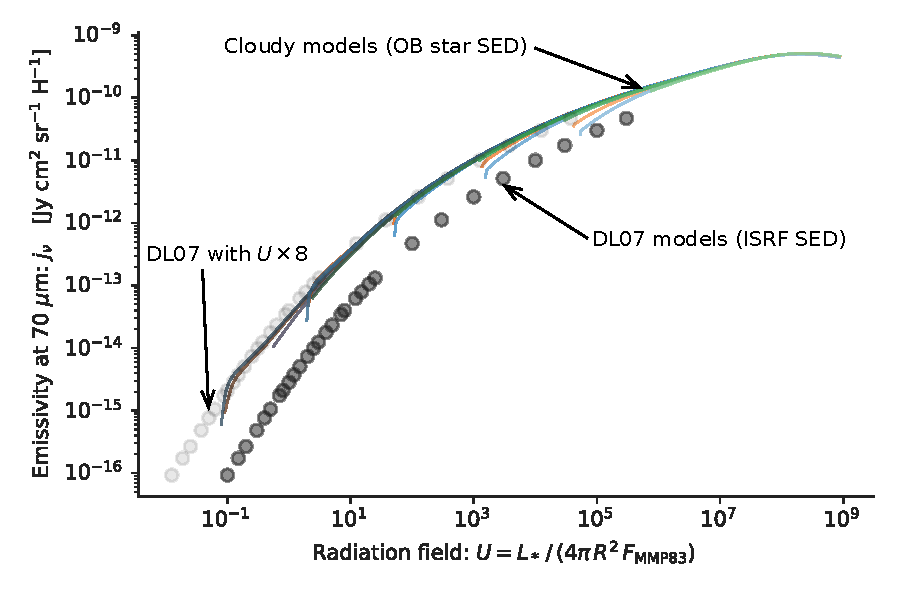
\includegraphics[width=\linewidth]{figs/grain-j70-vs-U-edited}
  \caption{Grain emissivity at \SI{70}{\um} for all Cloudy models
    (lines colored as in Fig.~\ref{fig:drift-gn}), compared with grain
    models from \citet{Draine:2007a} (dark gray symbols), which assume
    illumination by a scaled interstellar radiation field, which has a
    SED with a very different shape from that of an OB star, see
    Fig.~\ref{fig:sed-comparison}.  }
  \label{fig:grain-j70}
\end{figure}

The grain emissivity at \SI{70}{\um} (Herschel PACS blue band) for the
Cloudy simulations (colored lines) is shown in
Figure~\ref{fig:grain-j70}, where it is compared with the same
quantity from the grain models (dark gray symbols) of
\citet{Draine:2007a}.  A clear difference is seen between the two sets
of models, but this is due almost entirely to a difference in the
assumed spectrum of the illuminating radiation, as illustrated in
Figure~\ref{fig:sed-comparison}.  \citet{Draine:2007a} use a SED that
is typical of the interstellar radiation field in the Galaxy, which is
dominated by an old stellar population, which peaks in the near
infrared, with only a small FUV contribution from younger stars (about
8\% of the total energy density).  This is very different from the OB
star SEDs, which are dominated by the FUV and EUV bands.  Since the
grain absorption opacity is much higher at UV wavelengths than in the
visible/IR (see Fig.~\ref{fig:cloudy-ism-dust-opacity}), the effective
grain heating efficiency of the OB star SED is correspondingly higher.
The light gray symbols show the effect on the \citet{Draine:2007a}
models of multiplying the radiation field by a factor of \num{8} in
order to offset this difference in efficiency, which can be seen to
bring them into close agreement with the Cloudy models.  A further
difference is that the \citet{Draine:2007a} model includes small PAH
particles, which we do not include in our Cloudy models, since they
are believed to be largely absent in photoionized regions
\citep{Giard:1994a, Lebouteiller:2011a}.  However, this only effects
the emissivity at shorter mid-infrared wavelengths \(< \SI{20}{\um}\).

\begin{figure}
  \centering
  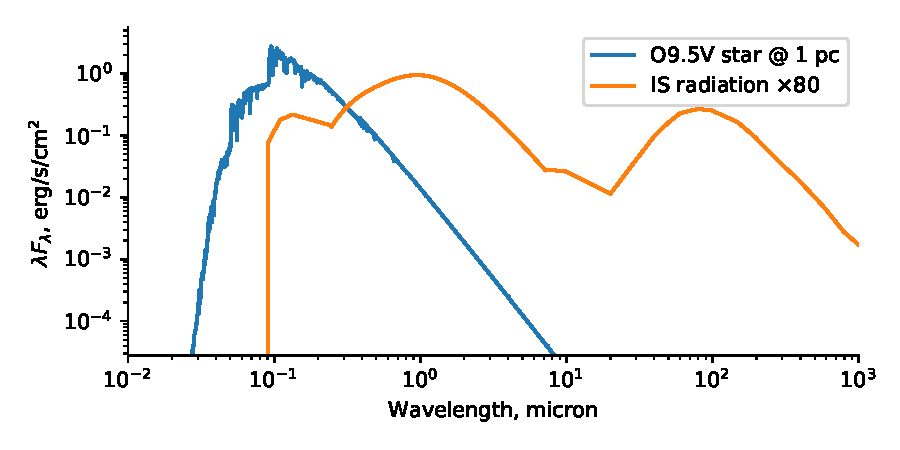
\includegraphics[width=\linewidth]{figs/sed-comparison}
  \caption{Comparison between the spectral energy distribution (SED)
    of a typical OB star (blue line) and the interstellar radiation
    field in the solar neighborhood (orange line).  The OB star is the
    \SI{20}{M_\odot} model from Table~\ref{tab:stars} and is plotted for a
    distance from the star of \SI{1}{pc}.  The interstellar SED is
    from \citet{Mathis:1983a} and is multiplied by \num{80} so that
    the total FUV-to-NIR flux is equal for the two SEDs.}
  \label{fig:sed-comparison}
\end{figure}

In terms of the characteristic parameters introduced in
\S~\ref{sec:depend-stell-type} the dimensionless radiation field becomes
\begin{equation}
  \label{eq:U-from-L4-and-Rpc}
  U = 14.7\, L_4\, R_{\text{pc}}^{-2} \ ,
\end{equation}
or, alternatively, it can be expressed in terms of the ambient stream as
\begin{equation}
  \label{eq:U-from-ambient}
  U = 3.01 \, n \, v_{10}^2 / x^2 \ , 
\end{equation}
where \(x = R_0/R_*\) is given by equation~\eqref{eq:x-cases}.  It can
also be related to the radiation parameter \(\Xi\), defined in
equation~\eqref{eq:Xi-Prad-over-Pgas}, as
\begin{equation}
  \label{eq:U-vs-Xi}
  U = 3.82 \, n T_4 \, \Xi \ .
\end{equation}
A common alternative approach to scaling the radiation field (see
\citealp{Tielens:1985a} and citations thereof) is to normalize in the
FUV band (\SIrange{0.0912}{0.24}{\um}), where the local interstellar
value is known as the Habing flux \citep{Habing:1968a}:
\begin{equation}
  \label{eq:Habing-flux}
  F\Hab = \SI{0.0016}{erg.s^{-1}.cm^{-2}} \ .
\end{equation}
The resultant dimensionless flux is often denoted by \(G_0\), and the
relationship between \(G_0\) and \(U\) depends on the fraction
\(f_{\text{fuv}}\) of the stellar luminosity that is emitted in the
FUV band:
\begin{equation}
  \label{eq:G-vs-U}
  G_0 = f_{\text{fuv}} \frac{u\mmp\, c}{F\Hab} \,U = (\text{\numrange{6}{10}}) \,U \ ,
\end{equation}
where we give the range corresponding to early O (\(f_{\text{fuv}} \approx 0.4\)) to early B (\(f_{\text{fuv}} \approx 0.7\)) stars.

%% Single-photon heating of small grains

\subsection{Unimportance of other heating mechanisms}
\label{sec:unimp-other-heat}
The grain temperature in bows around OB stars is determined
principally by the steady-state equilibrium between the absorption of
stellar UV radiation (heating) and the thermal emission of infrared
radiation (cooling).  Other processes such as single-photon stochastic
heating, Lyman~\(\alpha\) line radiation, and post-shock collisional
heating can dominate in other contexts, but these are generally
unimportant for circumstellar bows, as we now demonstrate.

\subsubsection{Stochastic single-photon heating}

When the radiation field is sufficiently dilute, then a grain that
absorbs a photon has sufficient time to radiate all that energy away
before it absorbs another photon \citep{Duley:1973a}.  In this case,
the emitted infrared spectrum for \(\lambda < \SI{50}{\um}\) becomes
relatively insensitive of the energy density of the incident radiation
\citep{Draine:2001a}.  However, this is most important for the very
smallest grains.  From equation~(47) of \citet{Draine:2001a}, one
finds that grains with sizes larger than
\(a = \SI{0.005}{\um} = \SI{5}{nm}\) (the smallest size included in
our Cloudy models) should be close to thermal equilibrium for
\(U > 30\), which is small compared with typical bow shock values
(\(U = \text{\numrange{e3}{e6}}\)).  As mentioned above, PAHs are not
expected to be present in the interior of \hii{} regions.
\citealp{Desert:1990a} found them to be strongly depleted for
\(U > 100\) around O stars.  However, other types of ultra-small
grains, down to sub-nm sizes \citep{Xie:2018a} may be present in bows,
and stochastic heating \emph{would} be important for grains with
\(a = \SI{1}{nm}\) if \(U < \num{e5}\).  Note, however that grains
smaller than \SI{0.6}{nm} would be destroyed by sublimation after
absorbing a single He-ionizing photon.


\subsubsection{Lyman \(\alpha\) heating}

On the scale of an entire \hii{} region, the dust heating is typically
dominated by Lyman \(\alpha\) hydrogen recombination line photons, which
are trapped by resonant scattering (e.g., \citealp{Spitzer:1978a}
\S~9.1b).  However, this is no longer true on the much smaller scale
of typical bow shocks.  An upper limit on the Lyman \(\alpha\) energy
density can be found by assuming all line photons are ultimately
destroyed by dust absorption rather than escaping in the line wings
(e.g., \citealp{Henney:1998b}), which yields
\begin{equation}
  \label{eq:U-Lya}
  U\Lya \approx 0.1 n / \kappa_{600} \ .
\end{equation}
This can be combined with equation~\eqref{eq:U-from-ambient} to give
the ratio of Lyman \(\alpha\) to direct stellar radiation as
\begin{equation}
  \label{eq:Lya-over-stellar}
  \frac{U\Lya}{U} \approx 0.03 \frac{x^2}{v_{10}^2 \kappa_{600}} \ .
\end{equation}
Taking the most favorable parameters imaginable of a slow stream
(\(v_{10} = 2\)), very strong wind (\(x \approx 1\)), and reduced dust
opacity (\(\kappa_{600} = 0.1\)) gives a Lyman \(\alpha\) flux of only 10\% of the
stellar flux.  In any other circumstances, the fraction would be even
lower.

\subsubsection{Shock heating}
\newcommand\kin{\ensuremath{_{\text{kin}}}}
The outer shock thermalizes the kinetic energy of the ambient stream,
which may in principle contribute to the infrared emission of the bow.
In order for this process to be competitive, the following three
conditions must all hold:
\begin{enumerate}[1.]
\item The post-shock gas must radiate efficiently with a cooling
  length less than the bow size, see \S~\ref{sec:radi-cool-lengths}.
  This is satisfied for all but the lowest densities (see
  Fig.~\ref{fig:zones-v-n-plane}).
\item A significant fraction of the shock energy must be radiated by
  dust.  This requires that the post-shock temperature be greater than
  \SI{e6}{K}, which requires a stream velocity
  \(v > \SI{200}{km.s^{-1}}\) \citep{Draine:1981a}.  This also
  coincides with the range of shock velocities where the smaller
  grains will start to be destroyed by sputtering in the post-shock
  gas.
\item The kinetic energy flux through the shock must be significant,
  compared with the fraction of the stellar radiation flux that is
  absorbed and reprocessed by the bow shell.
\end{enumerate}
It turns out that the third condition is the most stringent, so we
will consider it in detail.  The kinetic energy flux through the outer shock for an ambient stream of density \(\rho\) and velocity \(v\) is
\begin{equation}
  \label{eq:Fkin}
  F\ke = \tfrac12 \rho v^3 = \tfrac12 P\shell v \ , 
\end{equation}
while the stellar radiative energy flux absorbed by the shell is
\begin{equation}
  \label{eq:Ftrap}
  F\trap \approx \tau L / 4 \pi R_0^2 \ ,
\end{equation}
assuming an absorption optical depth \(\tau \ll 1\). The shell
pressure in the WBS case can be equated to the ram pressure of the
internal stellar wind (see \S~\ref{sec:three-bow-regimes}), so that
the ratio of the two energy fluxes is
\begin{equation}
  \label{eq:F-ratio-shock}
  \frac{F\ke}{F\trap} = \frac12 \frac{\eta\wind}{\tau} \frac{v}{c} \ .
\end{equation}
An upper limit to the stellar wind momentum efficiency \(\eta\wind\)
is the shell momentum efficiency \(\eta\shell\) that is derived
observationally in \S~\ref{sec:summary-discussion}, where it is found
that \(\eta\shell / \tau < 30\) for all sources considered.  Therefore,
for a stream velocity \(v = \SI{200}{km.s^{-1}}\), we have
\(F\ke/F\trap < 0.01\) and the shock-excited dust emission is still
negligible.  Only in stars with \(v > \SI{1000}{km.s^{-1}}\) would the
shock emission start to be significant, and such hyper-velocity stars
\citep{Brown:2015a} do not show bow shocks.

% Inner shock \dots no dust \dots proton Larmor radius very small, so
% no penetration across contact discontinuity

%%% Local Variables:
%%% mode: latex
%%% TeX-master: "dusty-bow-wave"
%%% End:


\section{Shape of a dusty radiative bow wave}
\label{sec:shape-dust-wave}

As an alternative to hydrodynamic or magnetohydrodynamic bow shocks,
it is possible that some observed emission arcs may be bow waves due
to the action of radiation pressure on dust grains.

\begin{figure}
  (a)\\
  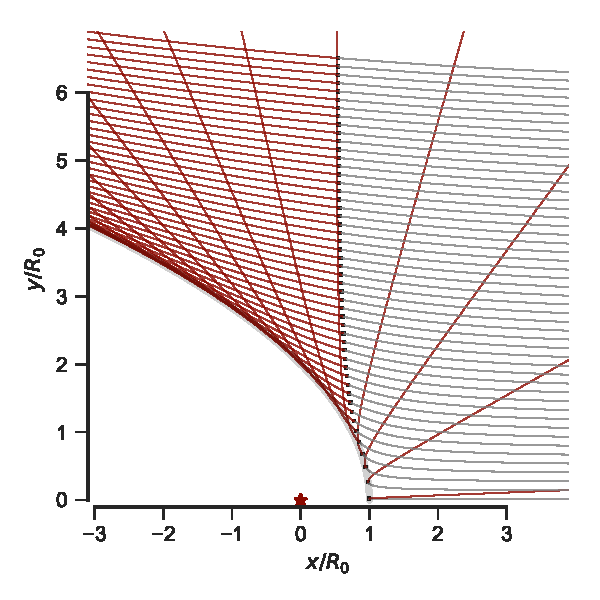
\includegraphics[width=\linewidth]{figs/dust-trajectories}
  (b)\\
  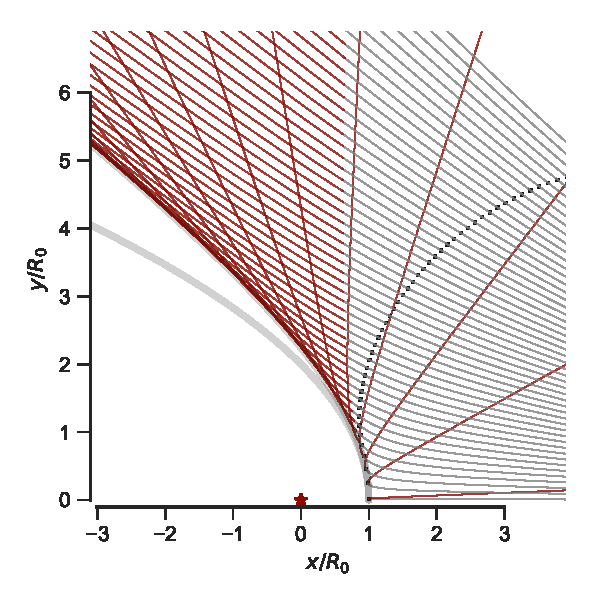
\includegraphics[width=\linewidth]{figs/dust-divergent}
  \caption[Dust grain trajectories]{Dust grain trajectories under
    influence of a repulsive central \(r^{-2}\) radiative force.
    (a)~A parallel stream of dust grains approach from the right at a
    uniform velocity and with a variety of impact parameters (initial
    \(y\)-coordinate). The central source is marked by a red star at
    the origin, and its radiative force deflects the trajectories into
    a hyperbolic shape, each of which reaches a minimum radius marked
    by a small black square.  The incoming hyperbolic trajectories are
    traced in gray and the outgoing trajectories are traced in red.
    The locus of closest approach of the outgoing trajectories is
    parabolic in shape (traced by the thick, light gray line) and this
    constitutes the inner edge of the bow wave.  (b)~The same but for
    a divergent stream of dust grains that originates from a source on
    the \(x\) axis at a distance \(D = 10 R_0\) from the origin.  In
    this case, the inner edge of the bow wave is hyperbolic and the
    parallel stream result is also shown for comparison.}
  \label{fig:dust-trajectories}
\end{figure}



A dust grain of geometrical cross-section \(\xsec\) situated a
distance \(R\) from a point source of radiation with luminosity \(L\)
will experience a repulsive, radially directed radiative force
\citep[e.g.,][]{Spitzer:1978a}
\begin{equation}
  \label{eq:dust-rad-force}
  \frad = \frac{\xsec \Qp L} {4 \pi R^2 c} e^{-\tau}
\end{equation}
where \Qp{} is the frequency-averaged\footnote{%
  Frequency averages of any quantity \(x\) should be understood as
  weighted by the attenuated source spectrum:
  \(\langle x \rangle_\nu = (L \, e^{-\tau})^{-1} \int_0^\infty x(\nu)\, L_\nu \, e^{-\tau_\nu} \, d\nu
  \).  } %
radiation pressure efficiency\footnote{%
  For absorption efficiency \(Q_{\text{abs}}\), scattering efficiency
  \(Q_{\text{scat}}\), and asymmetry parameter (mean scattering
  cosine) \(g\), we have
  \(\Qp = Q_{\text{abs}} + (1 - g) Q_{\text{scat}}\)
  \citep[e.g., \S~4.5 of][]{Bohren:1983a}.} %
of the grain, \(c\) is the speed of light, and \(\tau\) is the
frequency-averaged optical depth between the source and the grain.
For simplicity, we will consider only the optically thin case,
\(\tau \to 0\).

\subsection{Gas-free bow wave}
\label{sec:gas-free-bow}


If \(\frad\) is the only force experienced by the grain, then it will
move on a \textit{ballistic} trajectory, determined by its initial
speed at large distance, \(v_\infty\), and its impact parameter, \(b\).
For \(b = 0\), the grain radially approaches the source with initial
radial velocity \(-v_\infty\), which is decelerated to zero at the distance
of closest approach, \(R_0\), given by energy conservation:
\begin{equation}
  \label{eq:dust-r0}
  R_0 = \frac{\xsec \Qp L} {2 \pi c m\grain v_\infty^2} \ ,
\end{equation}
where \(m\grain\) is the grain mass.  The grain then turns round and
recedes from the source along the same radius, reaching a velocity of
\(+v_\infty\) at large distance.  For \(b > 0\), the trajectory,
\(R\grain(\theta; b)\), is found\footnote{%
  The problem is formally identical to that of Rutherford scattering,
  or (modulo a change of sign) planetary orbits.  The method of
  solution (via introduction of a centrifugal potential term and
  reduction to a 1-dimensional problem) can be found in any classical
  mechanics text \citep[e.g.,][\S~14]{Landau:1976a}.} %
to be hyperbolic, characterized by an eccentricity,
\(\varepsilon = \bigl( 1 + 4 b^2 / R_0^2\bigr)^{1/2}\), and polar angle of
closest approach, \(\thm = \cos^{-1} \varepsilon^{-1}\).  The trajectory is
symmetrical about \(\thm\) and can be written as
\begin{equation}
  \label{eq:dust-r-theta}
  \frac{R\grain(\theta; b)} {R_0} = 
  \frac{ \tfrac12 \bigl( \varepsilon^2 - 1 \bigr)} {\varepsilon \cos(\theta - \thm) - 1} \ , 
\end{equation}
with a total deflection angle of \(2 \thm\), which is equal to
\ang{90} when \(b = 0.5 R_0\).

\subsubsection{Parallel dust stream}
\label{sec:dust-parallel}

If the incoming dust grains initially travel along parallel
trajectories with varying \(b\), but the same \(v_\infty\), then deflection
by the radiative force will form a bow wave around the radiation
source, as shown in Figure~\ref{fig:dust-trajectories}.  However, the
inner edge of the bow wave, \(R_{\text{in}}(\theta)\) is not given by the
closest approach along individual trajectories, \(R\grain(\thm; b)\),
but instead must found by minimizing \(R\grain(\theta; b)\) over all
\(b\) for each value of \(\theta\), which yields
\begin{equation}
  \label{eq:dust-r-in}
  \frac{R_{\text{in}}(\theta)} {R_0} = \frac{2}{1 + \cos\theta} \ .
\end{equation}
This is the polar form of the equation for the confocal parabola,
which we have already discussed in detail in \PaperI{}'s
\S~\ref{Q-sec:conic} and Appendix~\ref{Q-app:parabola}.  Its planitude
and alatude are \(\Gamma = \Lambda = 2\) and these are unchanged under projection
at any inclination.



\subsubsection{Divergent dust stream}
\label{sec:dust-divergent}

If the dust grains are assumed to originate from a second point
source, located at a distance \(D\) from the radiation source, then
the incoming stream will be divergent instead of plane parallel.  The
individual streamlines are not affected by this change and are still
described by equation~\eqref{eq:dust-r-theta}, except that the
trajectory axes for \(b > 0\) are no longer aligned with the global
symmetry axis, so we must make the substitution
\(\theta \to \theta + \theta_1(b)\), where \(\sin \theta_1 = b / D\) (see
Fig.~\ref{Q-fig:crw-schema} of \PaperI{}). We parametrize the degree
of divergence as \(\mu = R_0 / D\) and, as before,
\(R\grain(\theta + \theta_1(b, \mu); b)\) is minimized over all trajectories to
find the shape of the bow wave's inner edge.  This time, the result is
a confocal hyperbola:
\begin{equation}
  \label{eq:dust-divergent-r-in}
  \frac{R_{\text{in}}(\theta; \mu)} {R_0} = \frac{1 + \varepsilon_\mu}{1 + \varepsilon_\mu\cos\theta} \ ,
\end{equation}
where the eccentricity is (to first order in \(\mu\))
\( \varepsilon_\mu = (1 - 2\mu)^{-1}\).  An example is shown in
Figure~\ref{fig:dust-trajectories} for \(\mu = 0.1\).  Unsurprisingly,
the resulting bow shape is more open than in the parallel stream case,
increasingly so with increasing \(\mu\).  The planitude and alatude are
both equal: \(\Pi = \Lambda = 1 + \varepsilon_\mu\).

\newcommand\drag{\ensuremath{_{\text{drag}}}}
\newcommand{\gas}{\ensuremath{_{\text{gas}}}}
\newcommand{\drift}{\ensuremath{_{\text{drift}}}}
\newcommand\soundspeed{\ensuremath{c_{\text{s,gas}}}}


\begin{figure}
  \centering
  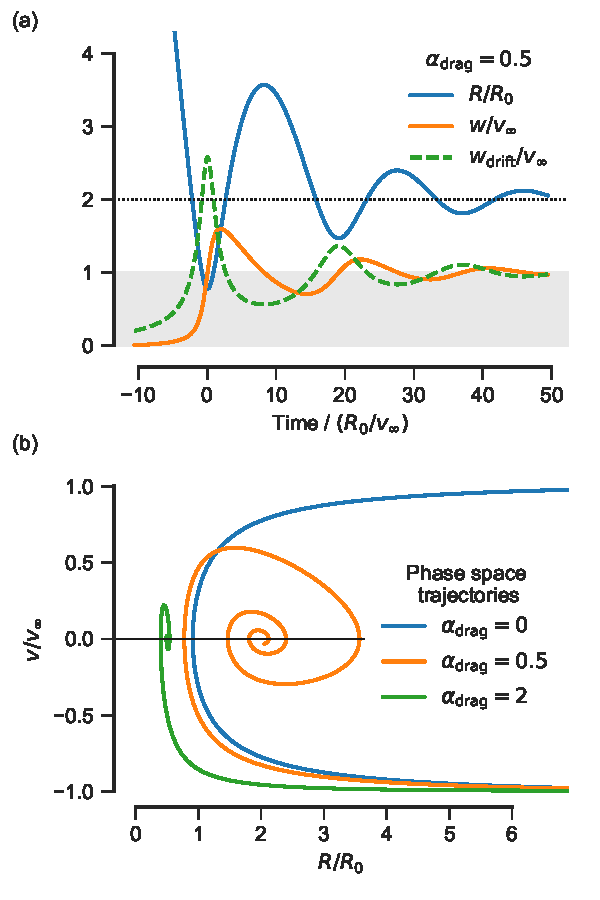
\includegraphics[width=\linewidth]{figs/dust-coupling-1d}
  \caption{Dust-gas coupling for an on-axis (purely radial)
    trajectory.  (a)~Grain radial position, \(R/R_0\), gas--grain
    velocity difference, \(w/v_\infty\), and local asymptotic drift
    velocity, \(w\drift/v_\infty\), versus time for
    \(\alpha\drag = 0.5\).  The behavior is typical of the dynamics of a
    damped harmonic oscillator. (b)~Phase space (position, velocity)
    trajectories for \(\alpha\drag = 0\), 0.5, and 2. All trajectories
    begin in the lower right corner and evolve in a clockwise
    direction. For \(\alpha\drag > 0\), the grain spirals in on the point
    \((x, u) = (\alpha\drag^{-1}, 0)\).}
  \label{fig:dust-coupling-1d}
\end{figure}

\begin{figure*}
  \centering
  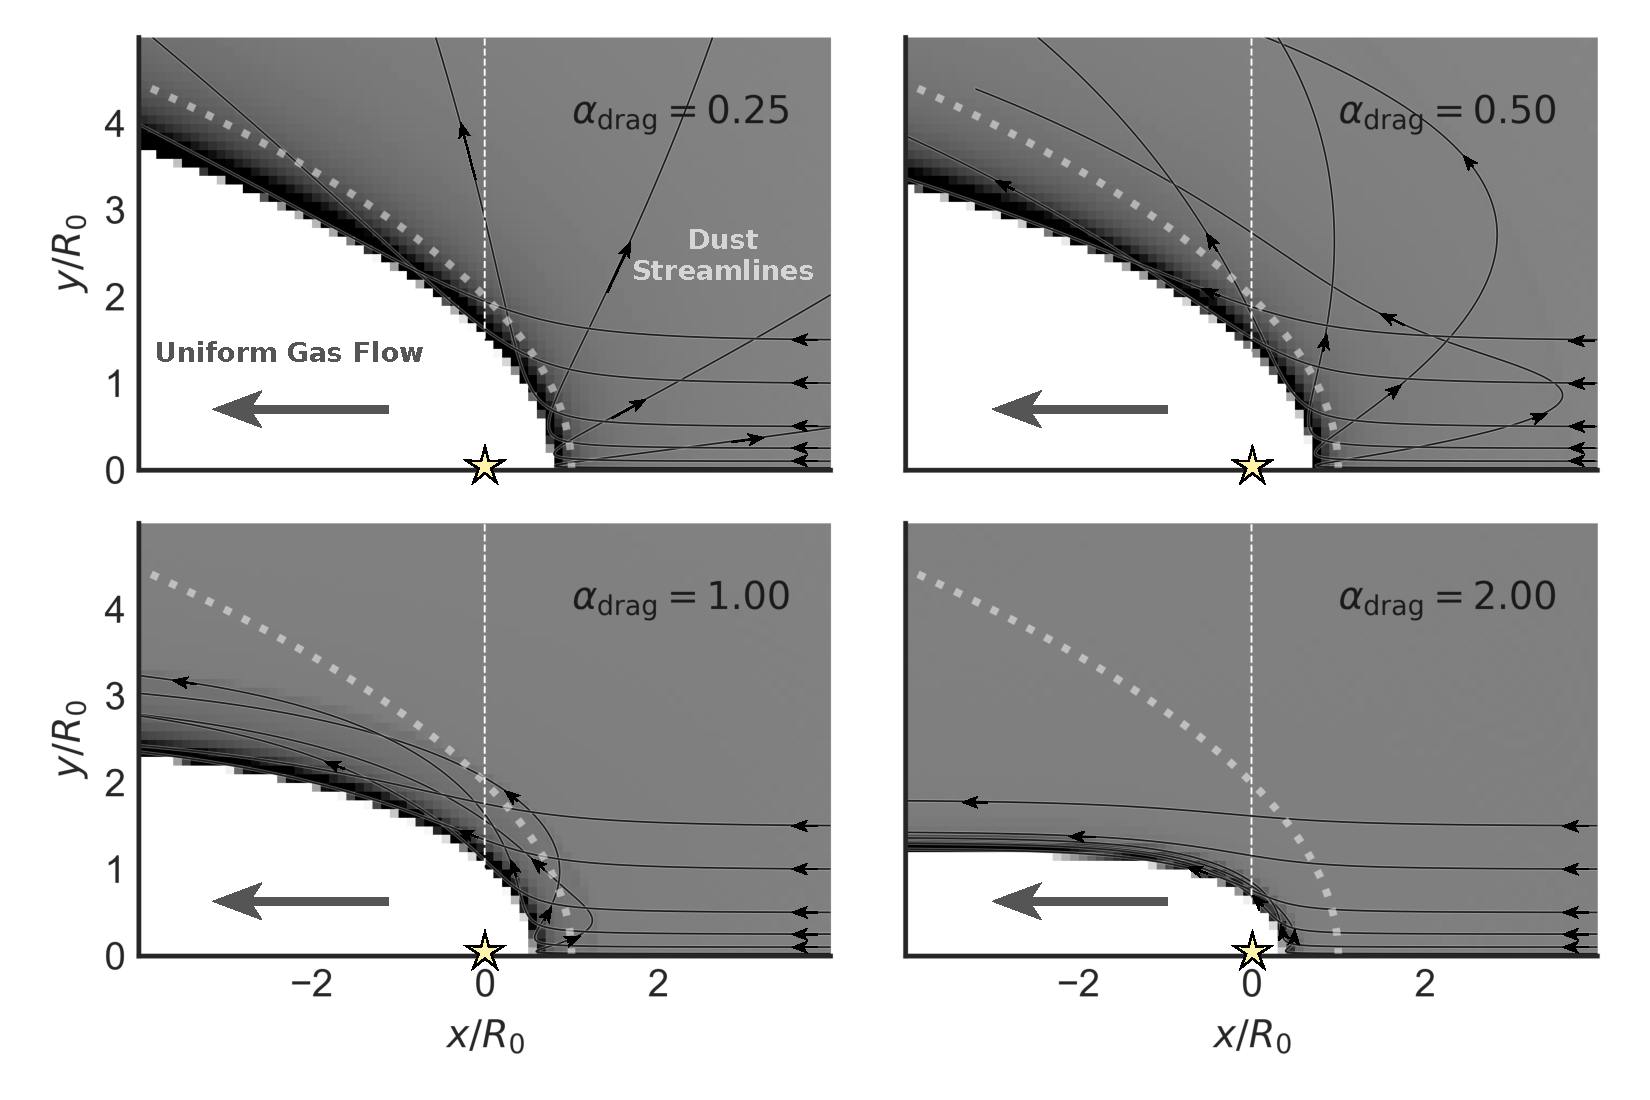
\includegraphics[width=\linewidth]{figs/dust-couple-stream-annotate}
  \caption{Dust grain trajectories under influence of gas drag in
    addition to a repulsive central radiative force.  The dust
    streamlines are shown as black lines with arrows and the dust
    density as a linear gray scale, with maximum (black) of twice the
    ambient dust density.  Results are shown for four values of the
    drag parameter (see text): \(\alpha_\text{drag} = 0.25\), \(0.5\),
    \(1.0\), and \(2.0\). The shape of the bow wave for the drag-free
    case (Fig.~\ref{fig:dust-trajectories}) is shown by the thick
    dotted line.  Faint patterns visible in the density away from the
    bow wave are numerical aliasing artefacts caused by sparse
    sampling of the streamlines in the low density regions.}
  \label{fig:dust-wave-coupling}
\end{figure*}


\subsection{Bow wave with gas drag}
\label{sec:bow-wave-drag}
More realistically, a grain will also be subject to a drag force,
\(f\drag\), due to its relative motion with respect to gas or plasma
particles. If the gas density, velocity, and sound speed are
\(\rho\gas\), \(v\gas\), and \(\soundspeed\), then a grain with velocity
\(v\grain\) will experience a drag force that is directed opposite to
the relative velocity, \(\bm{w} = \bm{v}\grain - \bm{v}\gas\).  In the
supersonic limit, \(w \equiv \abs{\bm{w}} \gg \soundspeed\), the magnitude of
the force is
\begin{equation}
  \label{eq:dust-fdrag}
  \abs{f\drag} \approx Q\drag \xsec \rho\gas w^2 \ ,
\end{equation}
where \(Q\drag\) is an efficiency factor (which may be smaller or
greater than unity) that accounts for details such as sticking
probability and the boost in cross section due to the Coulomb force
when a charged grain interacts with an ionized plasma
\citep{Draine:1979a}.  We neglect the back reaction of the dust on the
gas motion and assume a uniform background gas flow that is perfectly
coupled to the incoming dust stream at large radii.  So, for the
parallel stream case, we have \(\bm{v}\gas = -v_\infty \uvec{x}\) everywhere.

Considering the incoming flow on the symmetry axis, at each radius
there is an asymptotic gas--grain drift speed, \(w\drift\), for which
the radiative and drag forces exactly cancel, \(f\drag = -\frad\),
yielding
\begin{equation}
  \label{eq:dust-wdrift}
  w\drift = \left( \frac{\Qp L} {4\pi c Q\drag \rho\gas R^2} \right)^{1/2} \ .
\end{equation}
Any deviation of \(w\) from \(w\drift\) produces unbalanced forces
that tend to restore \(w \to w\drift\), although the grain inertia means
that this will not happen instantaneously, so that if \(w\drift\)
varies rapidly along a streamline, then changes in \(w\) will lag
behind.  We define a dimensionless coupling coefficient,
\(\alpha\drag\), to be the speed of the incoming stream in units of the
drift velocity at the radiative turn-around radius:
\begin{equation}
  \label{eq:dust-alpha}
  \alpha\drag \equiv \frac{v_\infty} {w\drift(R_0)} = \left(
    Q\drag \frac{R_0 / a\grain} {\rho\grain / \rho\gas}
  \right)^{1/2} \ ,
\end{equation}
where we have used equation~\eqref{eq:dust-r0} and suppressed a
grain-shape dependent geometric factor of order unity.  If
\(\alpha\drag \ll 1\), then \(w\drift \gg v_\infty\) out to several times the
turn-around radius, so the radiation field has no difficulty in
effectively decoupling the grain from the gas and producing the
velocity difference that is required to turn the grain around and
expel it towards the direction whence it came (\(w = 2 v_\infty\)).
However, for non-zero \(\alpha\drag\) the \(R^{-1}\) dependence of
\(w\drift\) (eq.~\eqref{eq:dust-wdrift}) means that the grain will
\textit{re-couple} to the inflowing gas stream around a radius
\(\approx R_0 / \alpha\drag \) and be swept back in again for another approach to
the source.  A further effect of increasing \(\alpha\drag\) is that the
grain penetrates closer to the star on its initial approach, thanks to
the tail wind provided by the gas flow.  Both these behaviors are
illustrated in Figure~\ref{fig:dust-coupling-1d}, where the inertial
lag of \(w\) behind \(w\drift\) means that the phase space trajectory
(panel b) is a spiral, which converges on the stagnation point
\((R, v) = (R_0 / \alpha\drag, 0)\). The cases \(\alpha\drag = 0.5\) and
\(\alpha\drag = 2\) are shown, and it can be seen that with larger
\(\alpha\drag\) the oscillations about the stagnation radius are
significantly damped.

However, this description only applies to grains with impact
parameter, \(b\), that is exactly zero.  Even a very small finite
\(b\) means that \(\frad\) has a component perpendicular to the axis,
which pushes the grain to the side and means that, after re-coupling,
its second approach is at a much larger impact parameter than its
first, so it is dragged around the wings of the bow wave before it can
bounce in and out more than twice.  This is illustrated in
Figure~\ref{fig:dust-wave-coupling}, which shows grain trajectories
and the resulting dust density structure, calculated from numerical
integration of equations~\eqref{eq:dust-rad-force}
and~\eqref{eq:dust-fdrag} in 2-D cylindrical coordinates.  Results are
shown for a range of coupling parameters, \(\alpha\drag\).  The
\(\alpha\drag = 0.25\) case appears qualitatively similar to the no-drag
case shown in Figure~\ref{fig:dust-trajectories}a, except that the
inner edge of the bow wave has been shifted to a smaller radius.
Recoupling of the outgoing streamlines to the gas flow does occur
eventually, but on length scales larger than shown in the figure. The
\(\alpha\drag = 0.5\) case shows the oscillating trajectories discussed
above for those grains that come in with a small initial impact
parameter.  In the \(\alpha\drag = 1.0\) case, the oscillating trajectories
are more confined, forming a thick shell around \(R_0\).  In the
\(\alpha\drag = 2.0\) case, the shell is much thinner and concentrated at
the inner rim.  As \(\alpha\drag\) increases, the oscillations are damped
further so that the stagnation radius \(R_0 / \alpha\drag\) becomes a good
approximation to the apex radius of the density wave.  All the cases
illustrated are for a parallel incident stream, but a divergent stream
gives qualitatively similar behavior, as shown in
Appendix~\ref{sec:equat-moti-grains}.  We propose the term
\textit{dragoid} for the 3-dimensional shapes of the bow waves, found
by rotating results such as Figure~\ref{fig:dust-wave-coupling} about
the symmetry axis.


\subsection{Applicability of the bow wave models}
\label{sec:dust-applicability}

The apex turn-around radius, \(R_0\), of the bow wave depends on the
grain properties via the combination \(\xsec \Qp / m\grain\).  For
grains of size \(a\grain\) and internal density \(\rho\grain\), we have
\(\xsec / m\grain \approx (a\grain \rho\grain)^{-1}\).  For radiation with
wavelength smaller than the grain size, \(\lambda < a\grain\), the
efficiency is \(\Qp \sim 1\), whereas for \(\lambda > a\grain\) it is
\(\Qp \sim a\grain/\lambda\).  Therefore, we would expect \(R_0\) to be almost
independent of grain size for small grains, but to vary as
\(R_0 \propto a\grain^{-1}\) for large grains, where small/large is relative
to the peak wavelength of the radiation source.  In principle, a
polydisperse population of grains could produce a blurring of the
observed bow wave, but only if large grains contribute significantly
to the dust emission.


\TODO{Variation of \(\alpha\drag\) with grain size, charged grains.}

\TODO{Lorentz force, Larmor radius}

\TODO{Back-reaction on gas, \(\alpha\drag \to \infty\), recovery of drag-free
  result for \(R_0\) but with increased effective grain mass.}

\subsection{Apparent shapes of projected dragoids}
\label{sec:dust-wave-apparent}

\begin{figure}
  \centering
  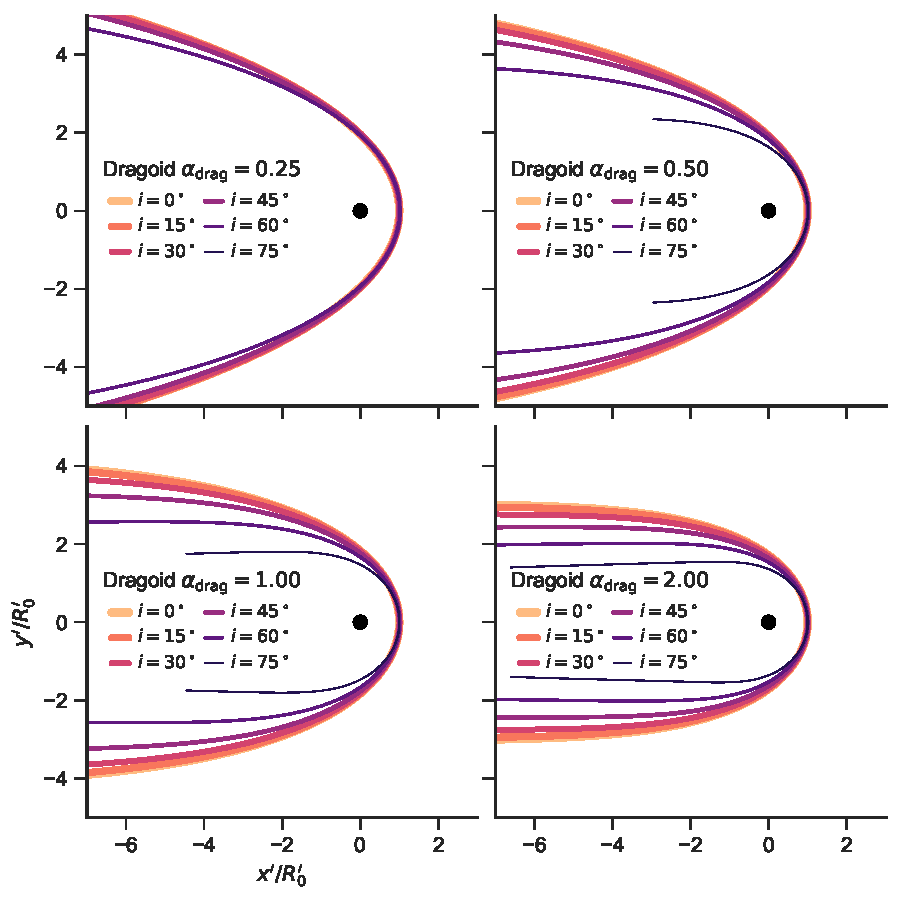
\includegraphics[width=\linewidth]{figs/test_xyprime_dragoid}
  \caption{Apparent bow shapes in the plane of the sky for
    parallel-stream dragoids as a function of inclination angle.  Drag
    coefficient, \(\alpha\drag\) increases from top-left to bottom-right.
    Inclination \(\abs{i}\) is shown in \ang{15} increments, indicated
    by line color and thickness (see key).}
  \label{fig:dragoid-xy-prime}
\end{figure}
\begin{figure}
  \centering
  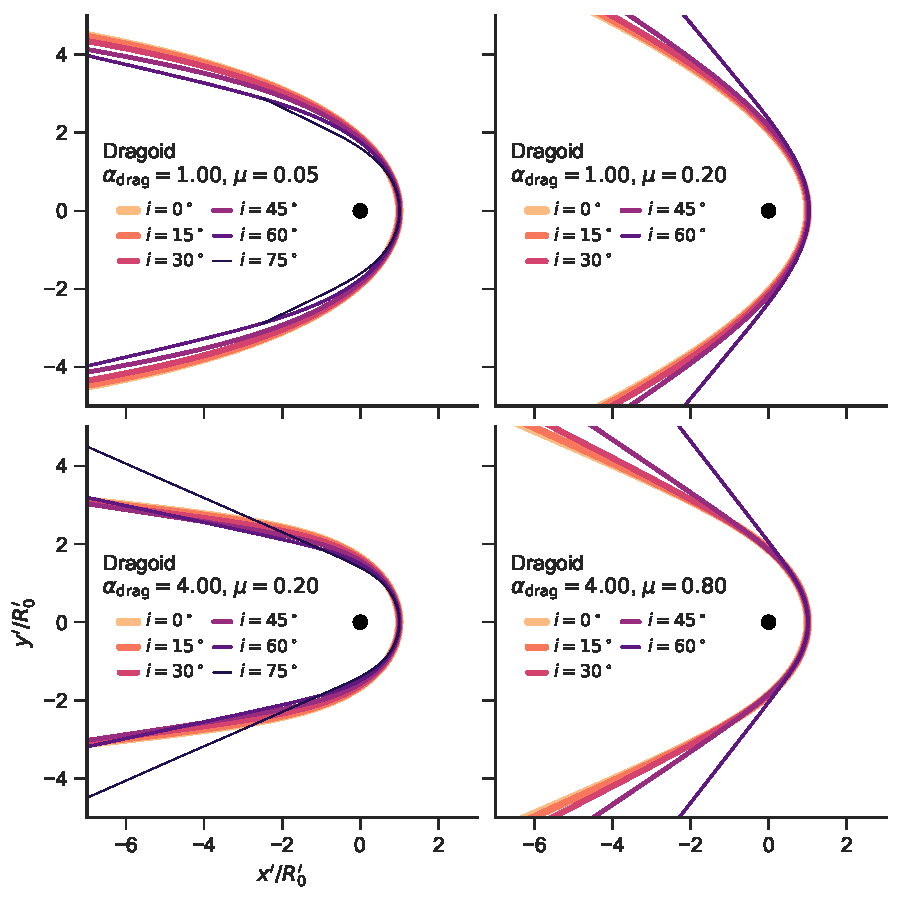
\includegraphics[width=\linewidth]{figs/test_xyprime_div_dragoid}
  \caption{As Fig.~\ref{fig:dragoid-xy-prime} but for divergent stream
    dragoids.  Drag coefficient increases from top to bottom, while
    degree of divergence increases from left to right. }
  \label{fig:dragoid-div-xy-prime}
\end{figure}


\begin{figure}
  \centering
  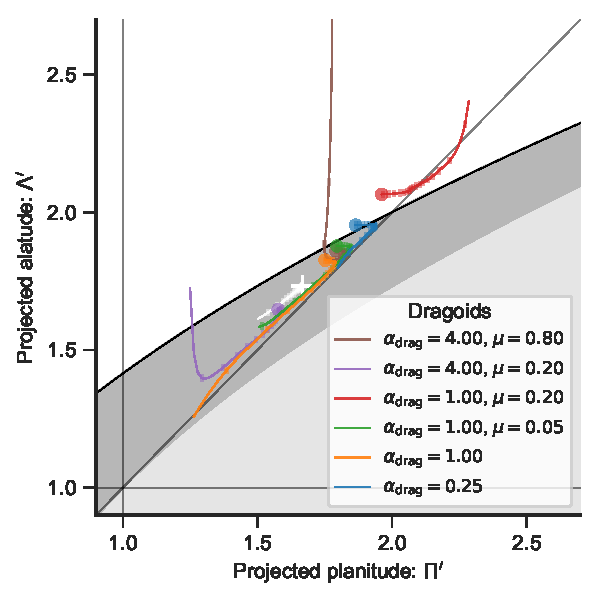
\includegraphics[width=\linewidth]{figs/dragoid-R90-vs-Rc}
  \caption{Apparent projected shapes of dragoids in the
    \(\Pi'\)--\(\Lambda'\) plane. Colored symbols indicate the
    \(\abs{i} = 0\) position for selected models (see key).  Thin
    lines show the inclination-dependent tracks of each model, with
    tick marks along each track for 20 equal-spaced values of
    \(\abs{\sin i}\). Gray shaded regions are as in
    Fig.~\ref{Q-fig:quadric-projection-continued}a of \PaperI{}.  The
    wilkinoid track is shown in white. }
  \label{fig:dragoid-Rc-R90}
\end{figure}

%%% Local Variables:
%%% mode: latex
%%% TeX-master: "dusty-bow-wave"
%%% End:

\section{Equations of motion for grains with radiation and gas drag}
\label{sec:equat-moti-grains}

\begin{figure}
  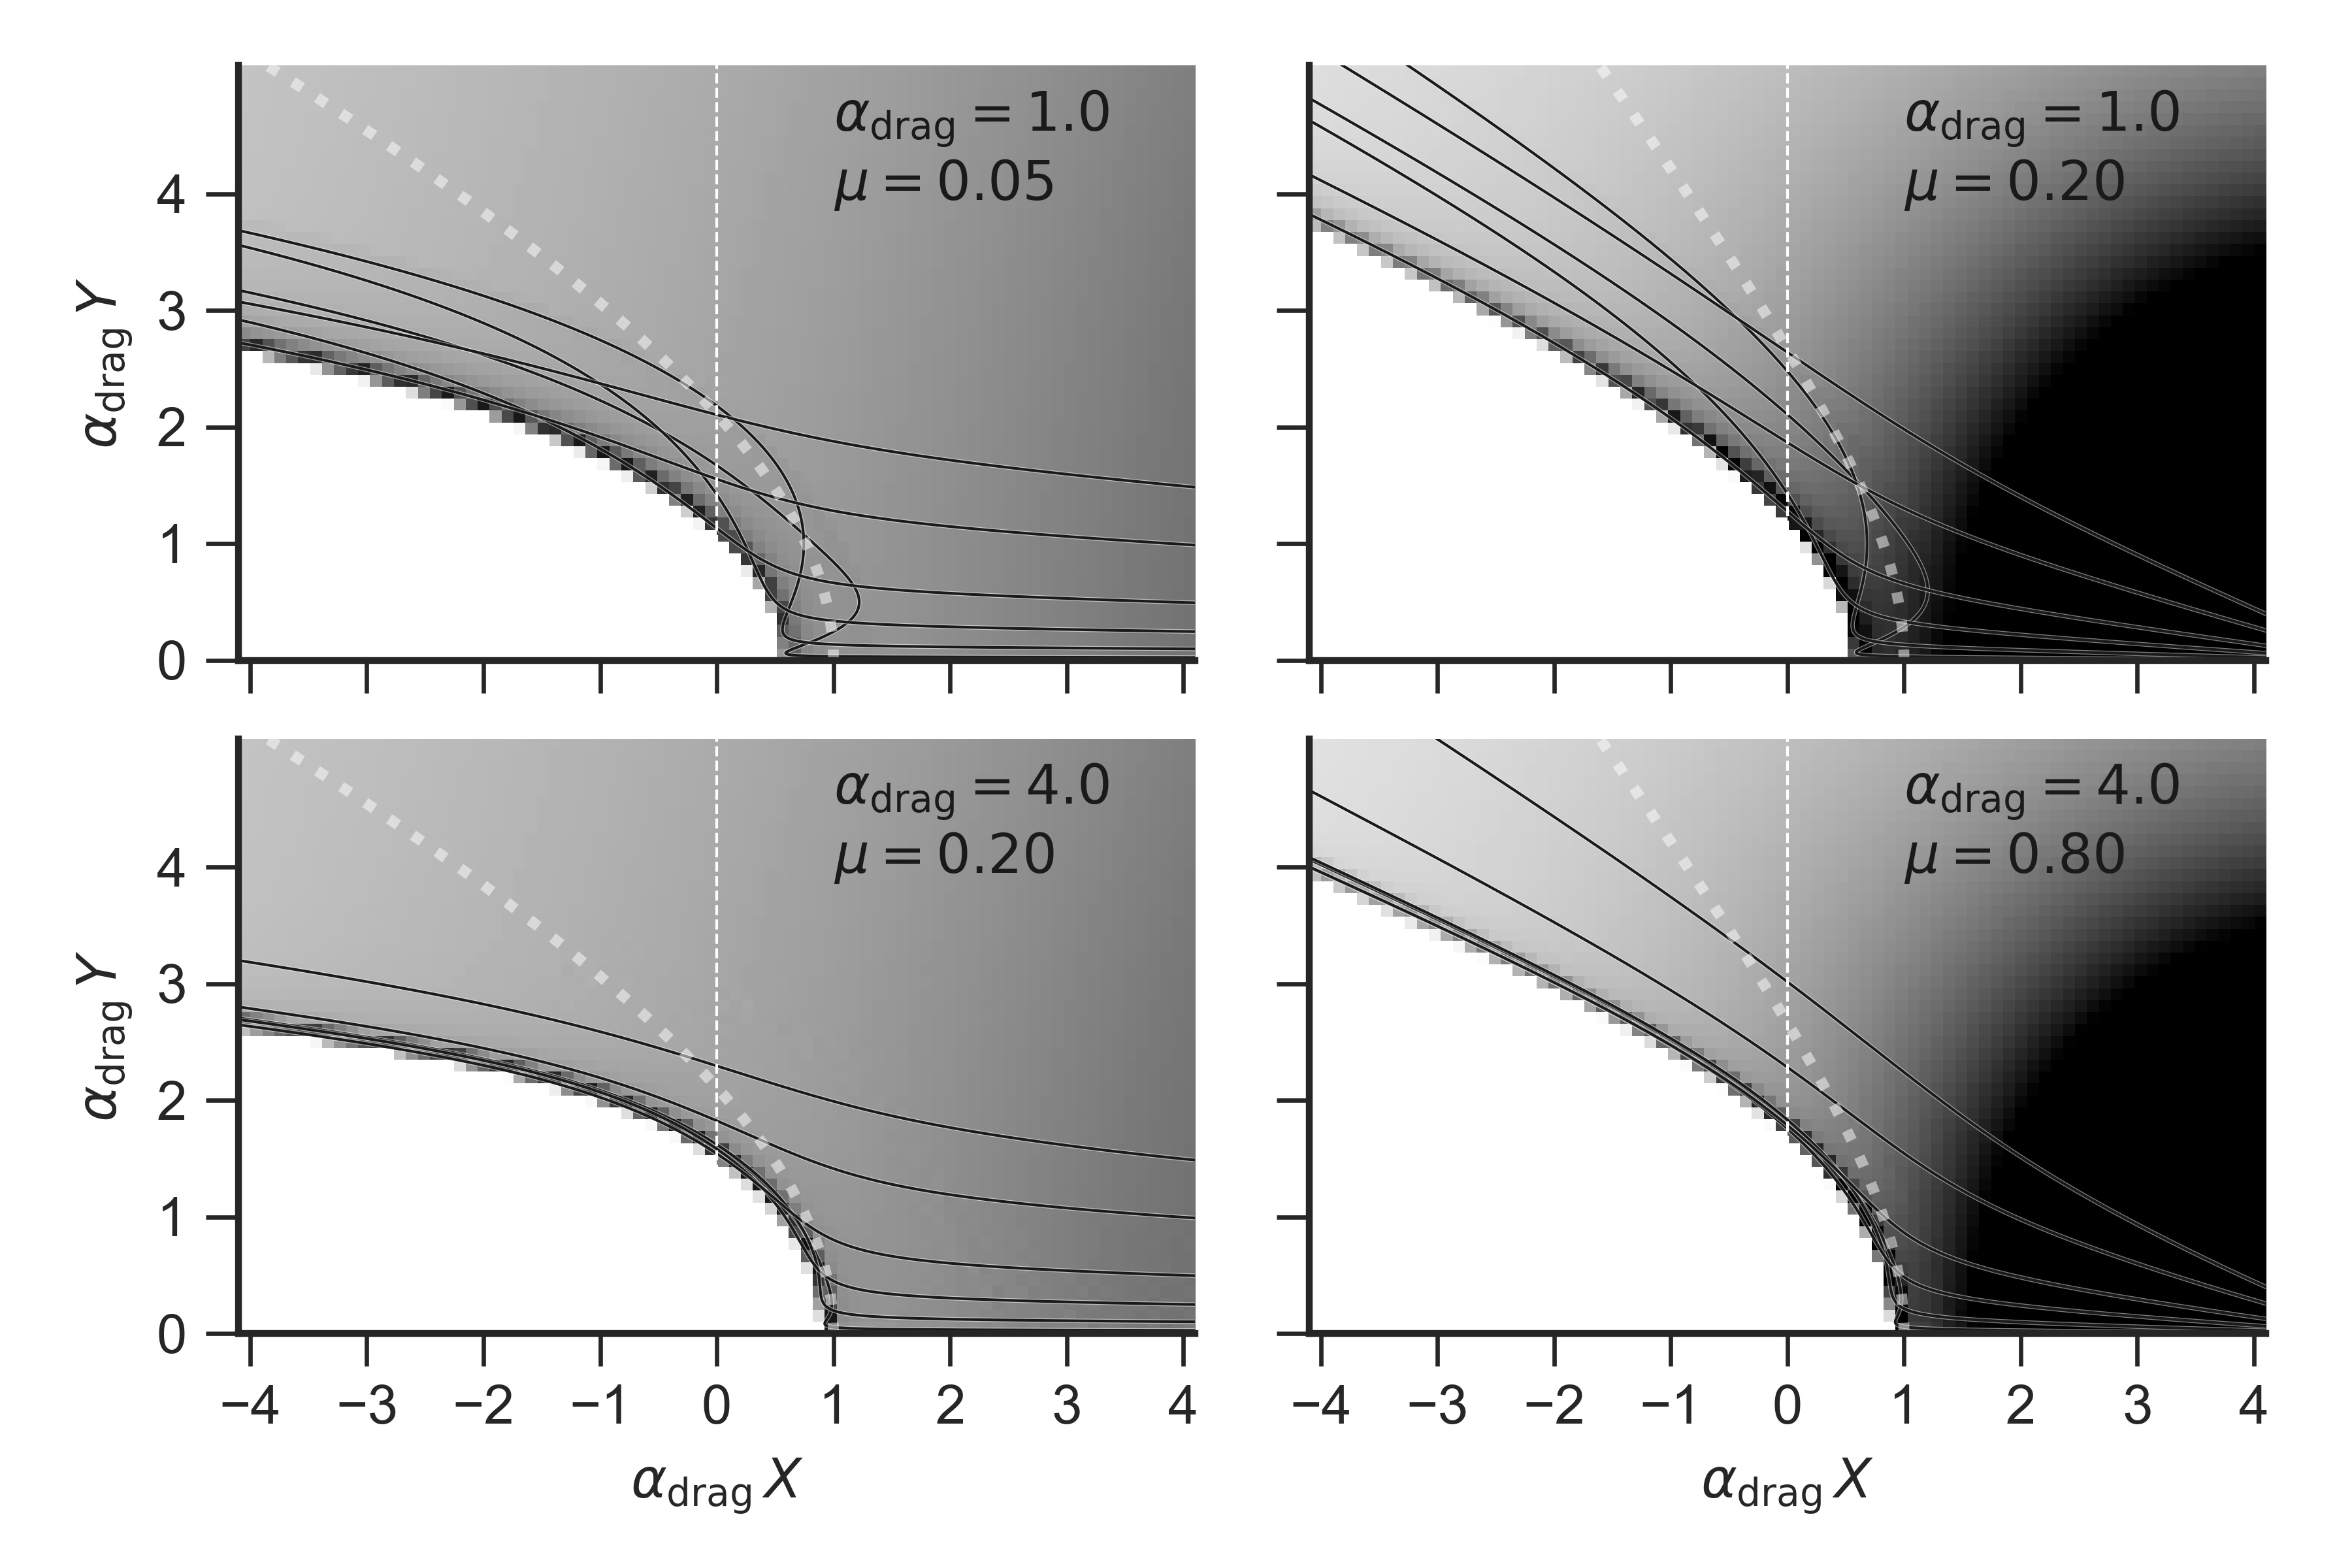
\includegraphics[width=\linewidth]{figs/dust-couple-div-stream}
  \caption{Divergent dragoids}
  \label{fig:divergent-dragoids}
\end{figure}

To find the dust grain trajectories \(R\grain(\theta)\) in the presence of
radiation and drag forces (\S~\ref{sec:bow-wave-drag}), we numerically
integrate the equations of motion. We define dimensionless cylindrical
polar coordinates,
\begin{equation}
  \label{eq:dust-XY}
  (X, Y) = \left(\frac{R\grain(\theta) \cos\theta } {R_0}, \ 
    \frac{R\grain(\theta) \sin\theta } {R_0}\right)
  \ ,
\end{equation}
and dust grain velocities,
\begin{equation}
  \label{eq:dust-UV}
  (U, V) = \left( \frac{\bm{v}\grain \cdot \uvec{x}} {v_\infty}, \ 
  \frac{\bm{v}\grain \cdot \uvec{y}} {v_\infty}\right) \ ,
\end{equation}
where \(\uvec{x}\) and \(\uvec{y}\) are unit vectors along the \(X\)
and \(Y\) axes (parallel and perpendicular, respectively, to the
symmetry axis).  The grain equation of motion then follows from
equations~(\ref{eq:dust-rad-force}, \ref{eq:dust-r0},
\ref{eq:dust-fdrag}--\ref{eq:dust-alpha}) as the following set of
coupled differential equations:
\begin{gather}
  \label{eq:dust-motion}
  \begin{aligned}
    \frac{d X}{d t} &= U \quad\quad
    \frac{d Y}{d t} = V \\
    \frac{d U}{d t} &= \frac12 \left[  
      X \left(X^2 + Y^2\right)^{-3/2} - \alpha\drag^2 D_1 \left(U - U_1\right)
    \right] \\
    \frac{d V}{d t} &= \frac12 \left[  
      Y \left(X^2 + Y^2\right)^{-3/2} - \alpha\drag^2 D_1 \left(V - V_1\right)
    \right] \ ,
  \end{aligned}
\end{gather}
where \((U_1, V_1)\) are the components of the gas velocity (assumed
fixed), given by
\begin{equation}
  \label{eq:dust-gas-velocities}
  (U_1, V_1) = 
  \begin{cases}
    \text{parallel stream} & (-1, 0)\\
    \text{divergent stream} &
    \left( \dfrac{X - \mu^{-1}}{R_1},\ \dfrac{Y}{R_1}\right) \ ,
  \end{cases}
\end{equation}
where
\begin{equation}
  \label{eq:dust-R1}
  R_1 = \left( \bigl(X - \mu^{-1}\bigr)^2 + Y^2 \right)^{1/2}
\end{equation}
is the distance from the second source, located at
\((X, Y) = (\mu^{-1}, 0)\).  The dimensionless gas density, \(D_1\),
normalized by the value at \((X, Y) = (1, 0)\), is
\begin{equation}
  \label{eq:dust-gas-density}
  D_1 = 
  \begin{cases}
    \text{parallel stream} & 1\\
    \text{divergent stream} & \dfrac{\bigl(\mu^{-1} - 1\bigr)^2} {R_1^{2}} \ .
  \end{cases}
\end{equation}

Equations~\eqref{eq:dust-motion} are integrated using the python
wrapper \texttt{scipy.integrate.odeint} to the Fortran ODEPACK library
\citep{Hindmarsh:1983a, Jones:2001a}, with results shown in
Figure~\ref{fig:dust-wave-coupling} for parallel-stream cases and
Figure~\ref{fig:divergent-dragoids} for divergent-stream cases. 

%%% Local Variables:
%%% mode: latex
%%% TeX-master: "dusty-bow-wave"
%%% End:

\section{Bow shock data from Kobulnicky et al. (2016, 2017, 2018)}
In a series of papers \citet{Kobulnicky:2016a, Kobulnicky:2017a,
  Kobulnicky:2018a} provide an extensive mid-infrared-selected sample
of over 700 candidate stellar bow shock nebulae.  For 20 of these
sources, reliable distances and spectral classifications are provided
(Table~5 of \citealp{Kobulnicky:2017a} and 
\citealp{Kobulnicky:2018a}), and these are used in
\S~\ref{sec:summary-discussion}, where we discuss the
\(\tau\)--\(\eta\) diagnostic diagram.  In this appendix, we outline our
treatment and analysis of the data in these catalogs, which differs in
some important respects from that of the original authors.

The most important quantity to be derived from the observations is the
absorption optical depth, \(\tau\), of the bow shell to the stellar radiation.


\begin{figure}
  \centering
  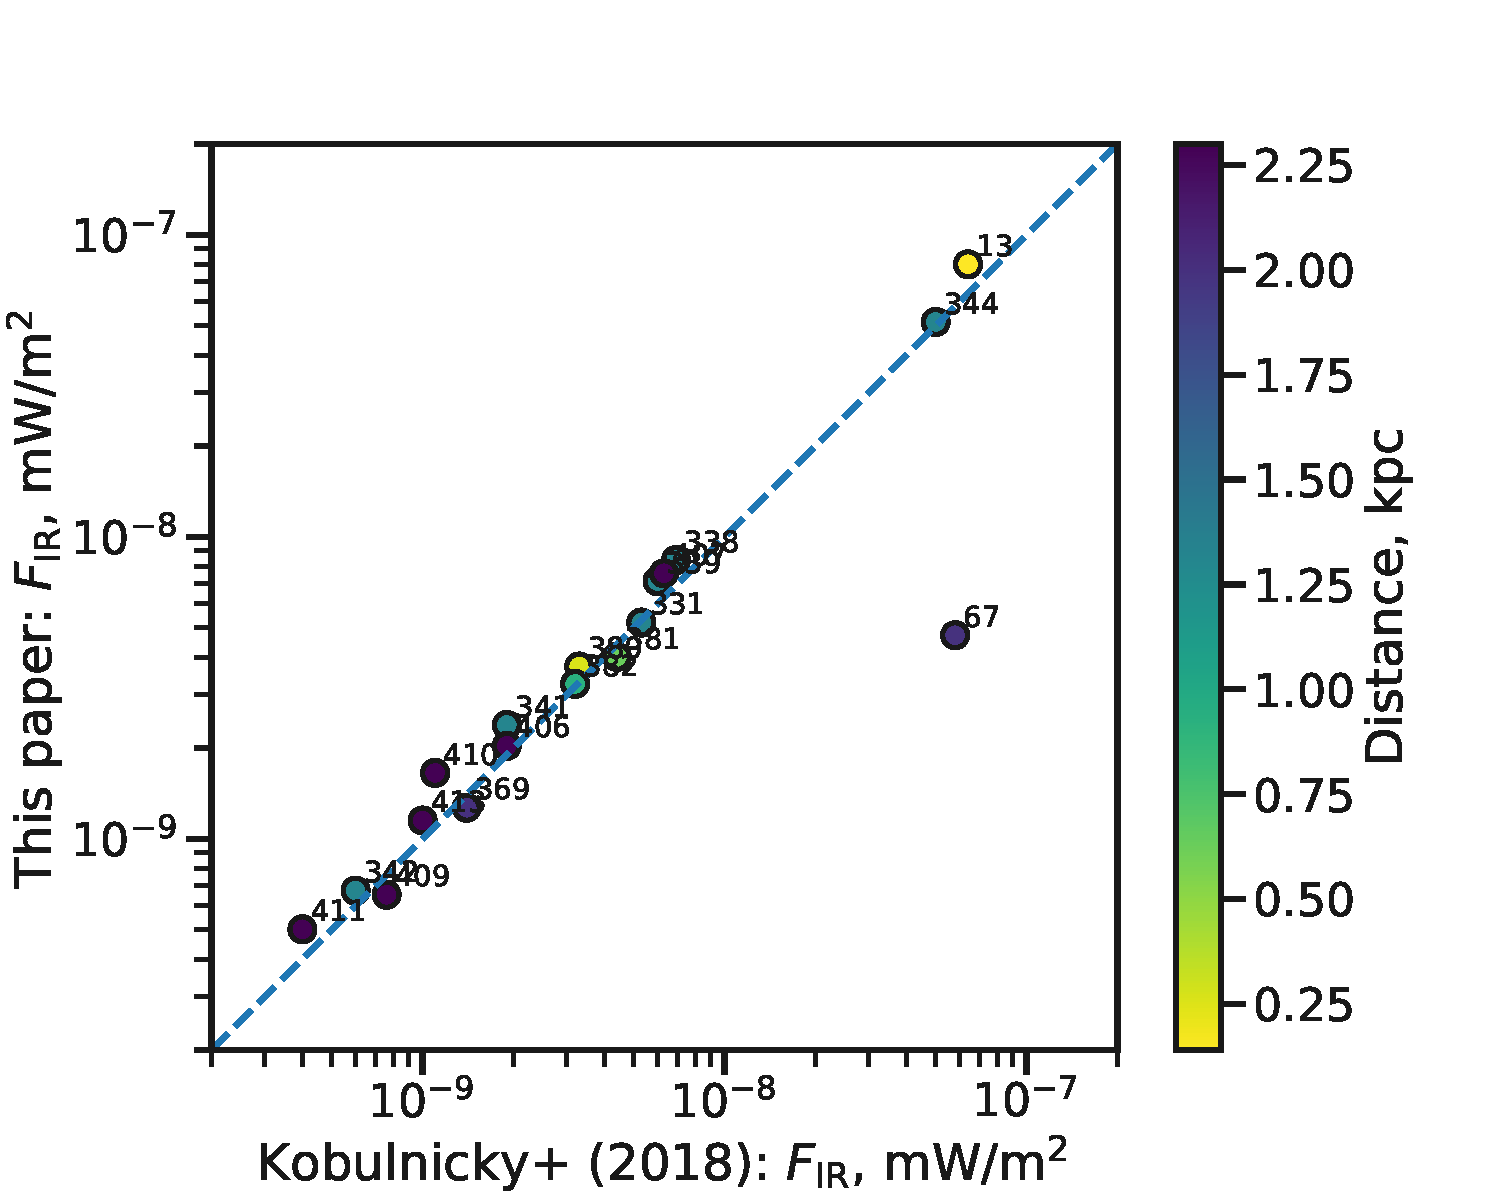
\includegraphics[width=\linewidth]{figs/K18-flux-comparison}
  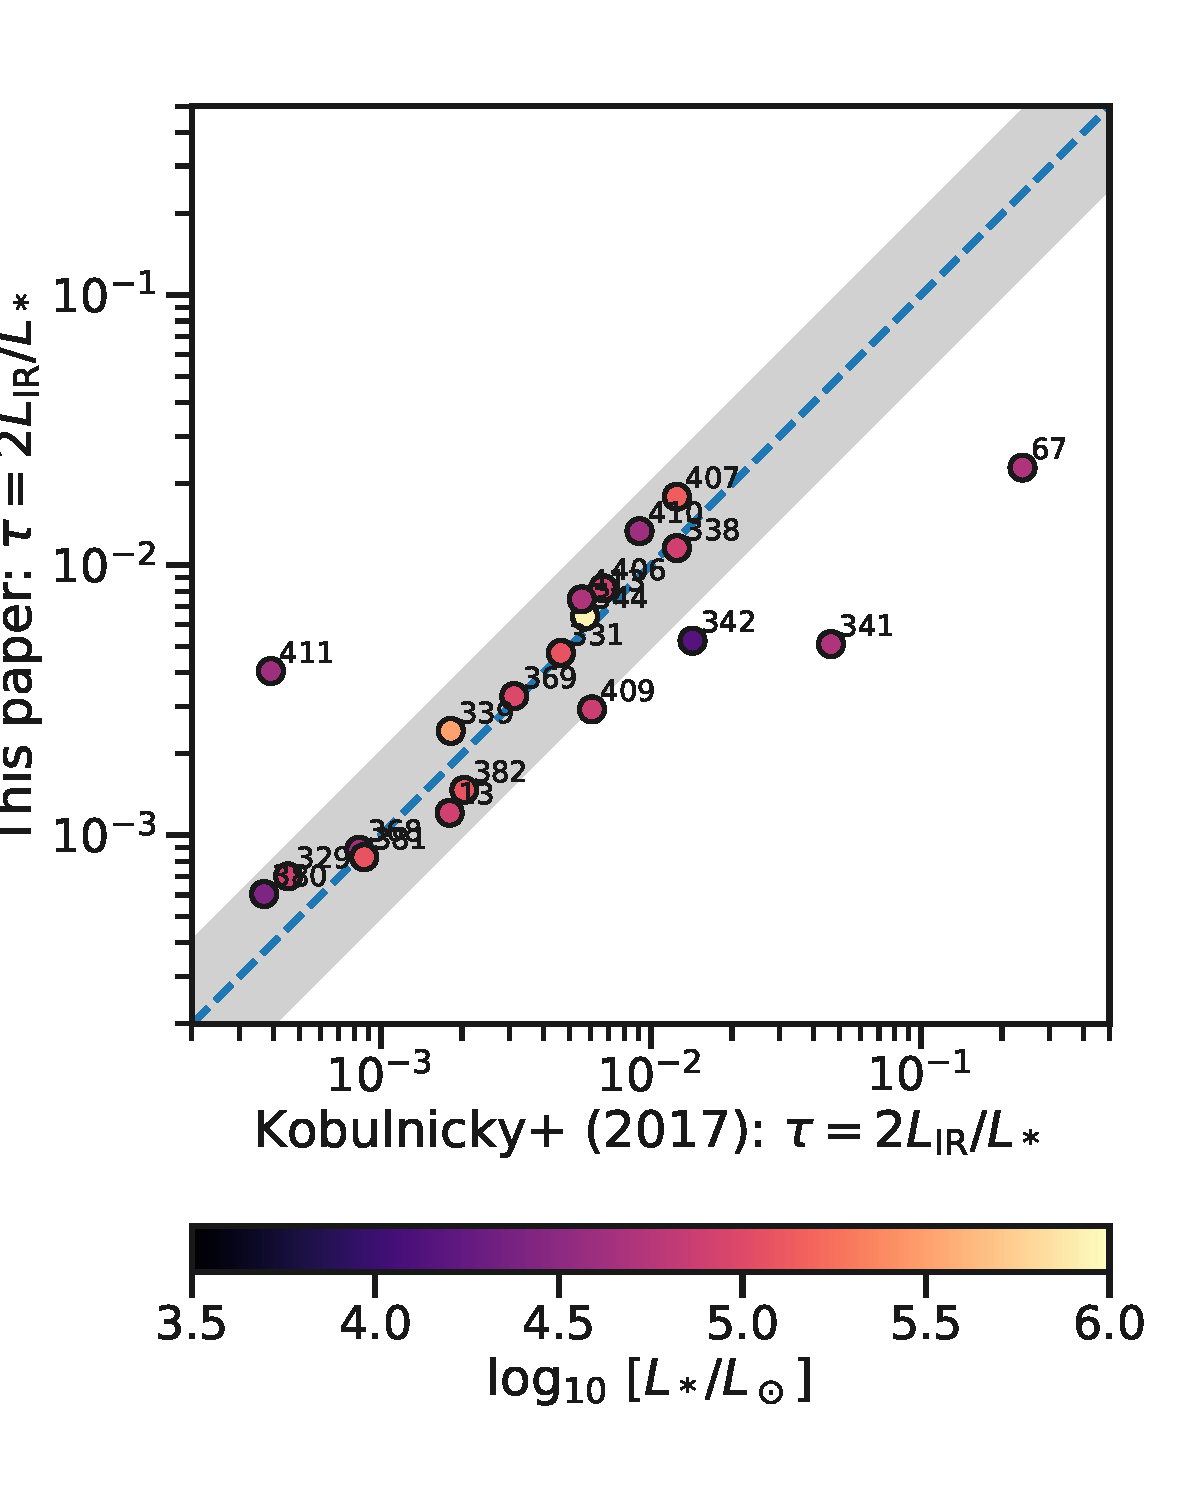
\includegraphics[width=\linewidth]{figs/K17-tau-comparison}
  \caption{Comparison}
  \label{fig:k17-k18-comparison}
\end{figure}

% So everything looks OK, except:

% * Source 67 is over 10 times too bright in the Kobulnicky table

% So, I will use my fluxes instead.  

\begin{figure*}
  \centering
  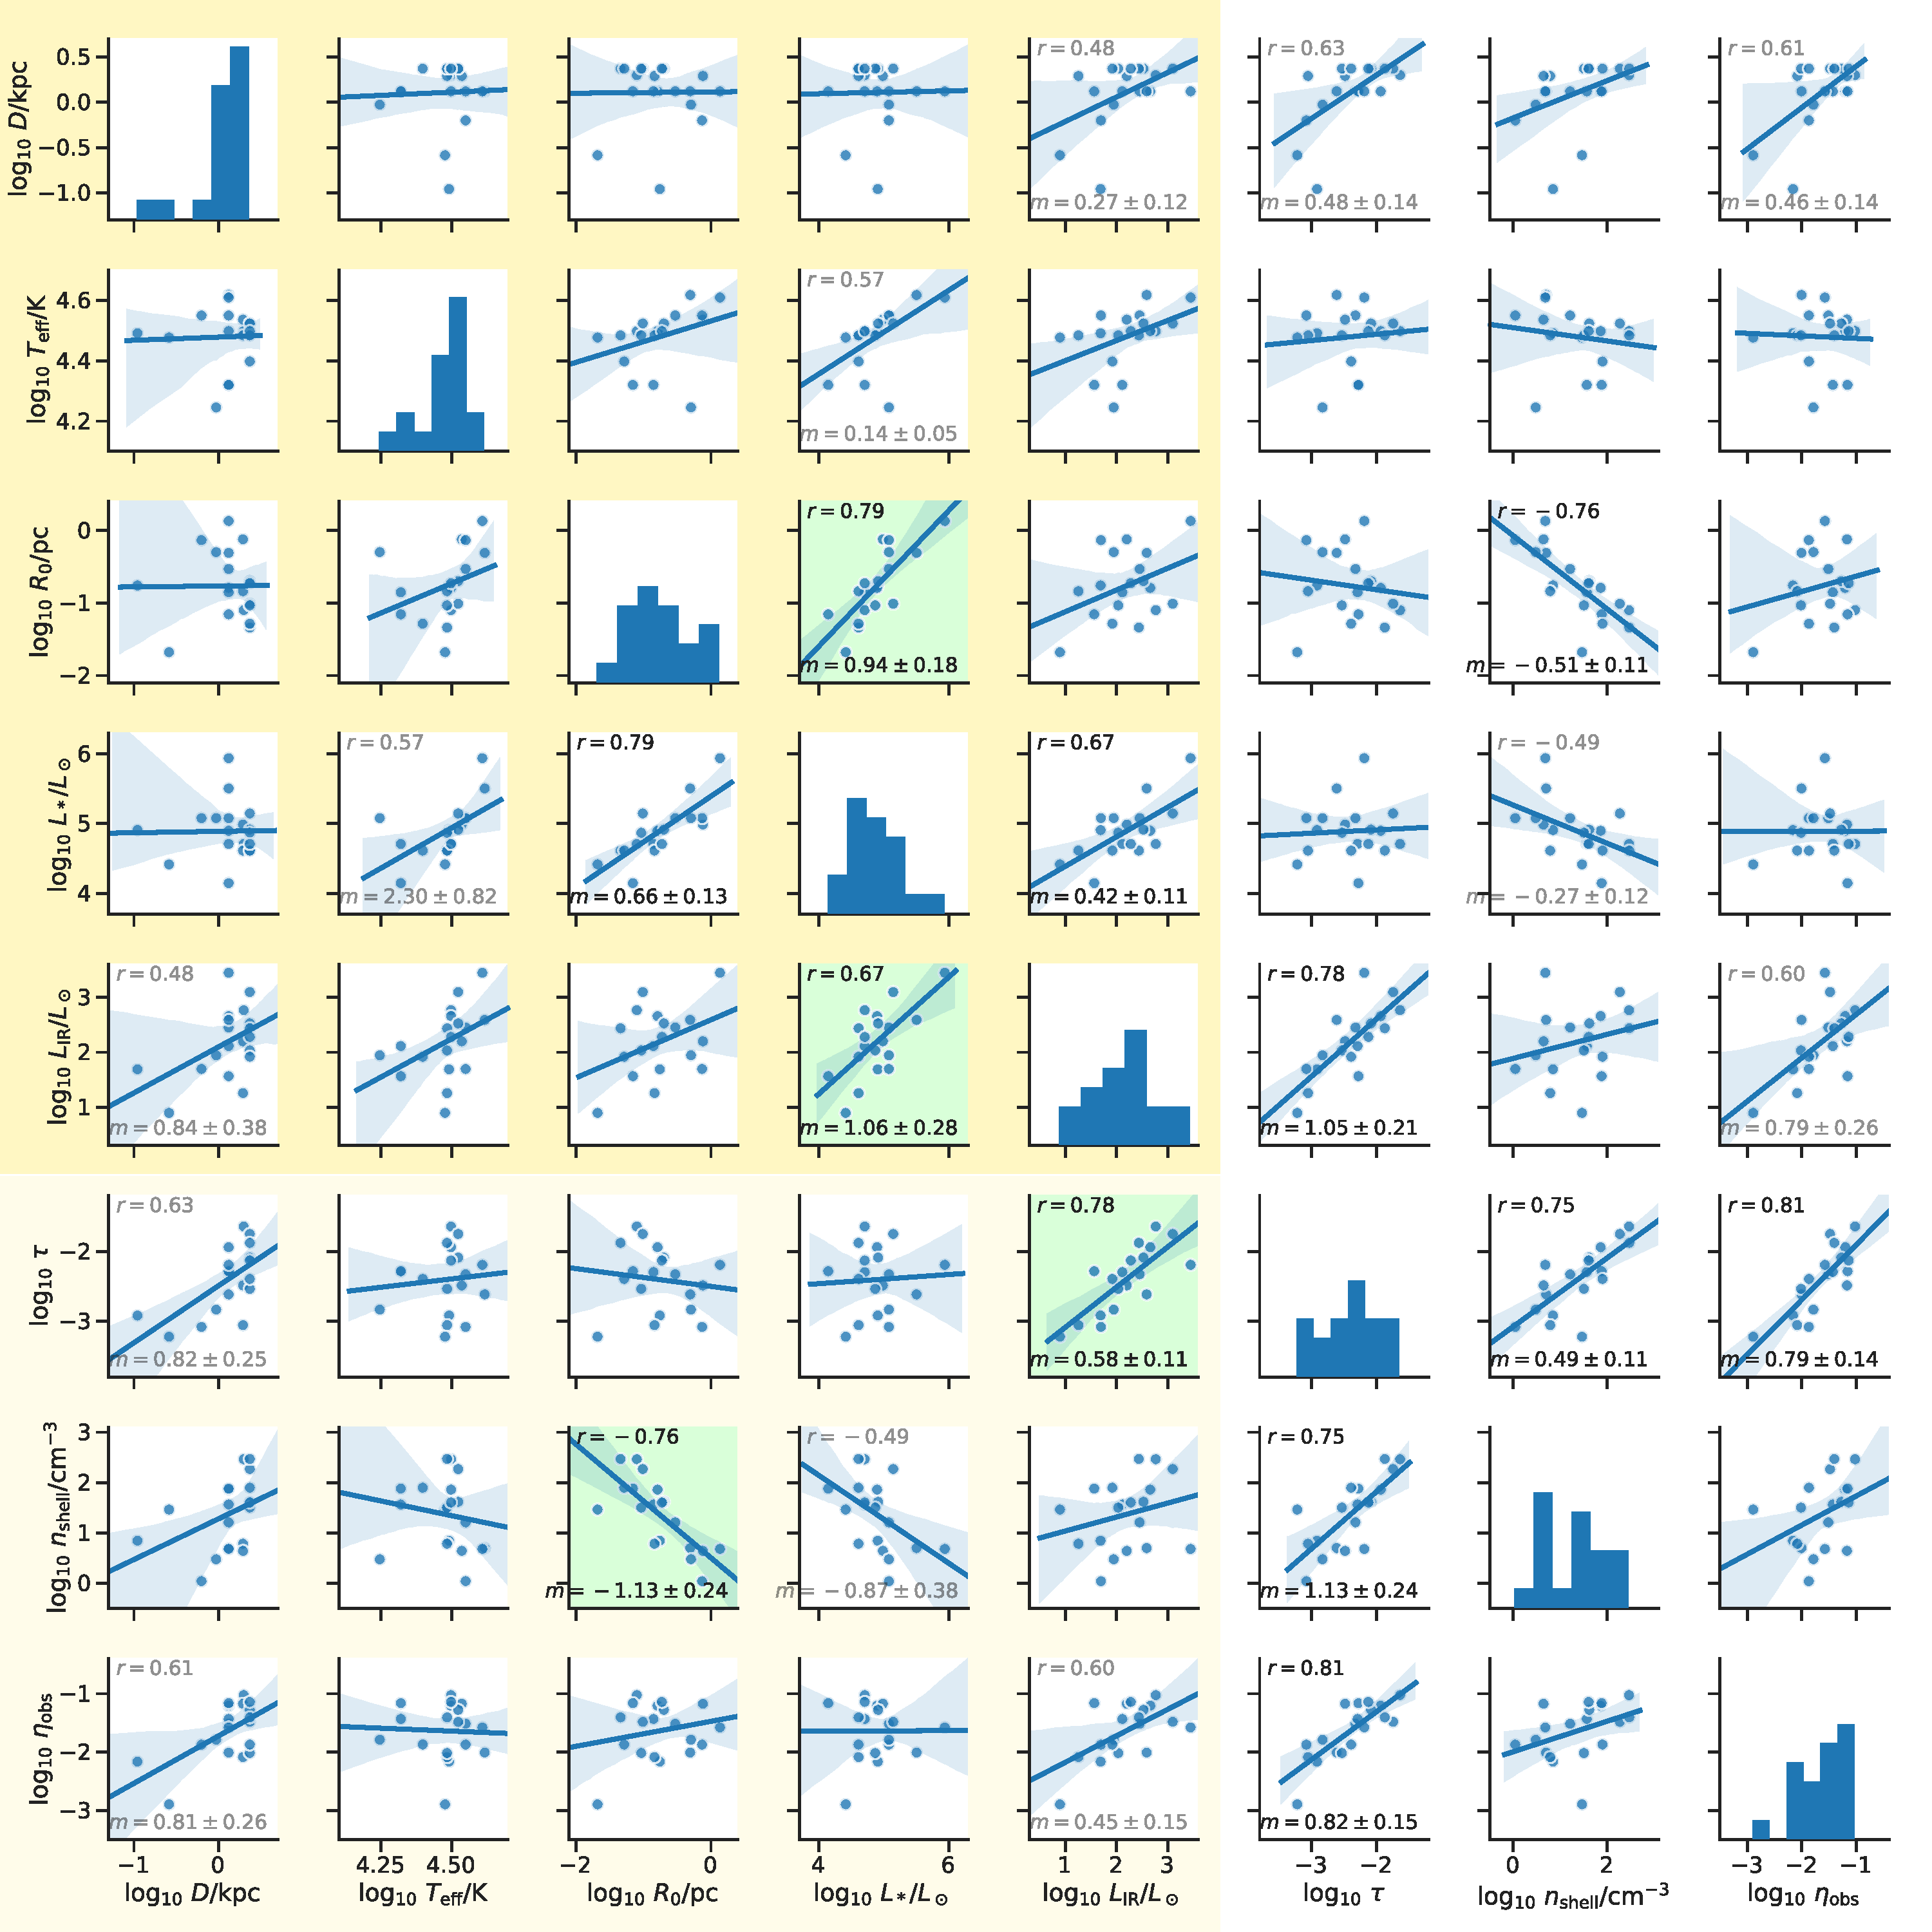
\includegraphics[width=\linewidth]{figs/K18-pairplot-edited}
  \caption[K18 pair plot]{Pair plots of correlations between observed
    and derived parameters of bows from the \citep{Kobulnicky:2018a}
    sample.}
  \label{fig:K18-pairplot-edited}
\end{figure*}


% In this graph we compare the original luminosity ratio taken directly from the Kobulnicky (2017) table (x axis) with the ratio calculated using my new total IR fluxes, combined with the new luminosities in the Kobulnicky (2018) table (y axis).   Most of the points show reasonable agreement between the two methods, with a few exceptions:

% * 67: this had the $F_\text{IR}$ overestimated in K17.  Using a more reasonable value gives a lower $\tau$
% * 341: The spectral class has changed from B2 (K17) to O9 (K18), increasing the assumed $L_*$, which lowers $\tau$
% * 411: The luminosity class has changed from Ib (K17) to V (K18), so $L_*$ has been greatly reduced, which increases the estimated $\tau$

% And there doesn't seem to be any significant correlation with stellar luminosity.

%%% Local Variables:
%%% mode: latex
%%% TeX-master: "dusty-bow-wave"
%%% End:

%
\section{Further details on ionization front trapping}
\label{sec:furth-deta-ioniz}

This appendix will probably be dropped from the paper.  It contains
details of the derivation of the ionization front trapping that I now
think are too verbose to be included, given that this is not the main
point of the paper.  They are collected here for completeness.

We wish to calculate whether the star is capable of photoionizing the
entire bow shock shell, or whether the ionization front will be
trapped within it.  The number of hydrogen recombinations\footnote{%
  The diffuse field is treated in the on-the-spot approximation,
  assuming all emitted Lyman continuum photons are immediately
  re-absorbed locally, so the case~B recombination co-efficient,
  \(\alphaB = \num{2.6e-13}\, T_4^{-0.7}\, \si{cm^3.s^{-1}}\), is
  used, where \(T_4 = T/\SI{e4}{K}\).} %
per unit time per unit area in a fully ionized shell is
\begin{equation}
  \label{eq:shell-recombination-rate}
  \mathcal{R} = \alphaB n\shell^2 h\shell \ ,
\end{equation}
while the flux of hydrogen-ionizing photons
(\(h \nu > \SI{13.6}{eV}\)) incident on the inner edge of the shell is
\begin{equation}
  \label{eq:shell-ionizing-flux}
  \mathcal{F} = \frac{S} {4 \pi R_0^2} \ , 
\end{equation}
where \(S\) is the ionizing photon luminosity of the star.  Any shell
with \(\mathcal{R} > \mathcal{F}\) cannot be entirely photoionized by
the star, and so must have trapped the ionization front.  The column
density of the shocked shell can be found, for example, from
equations~(10) and~(12) of \citet{Wilkin:1996a} in the limit
\(v_\infty/V \to 0\) (Wilkin's parameter \(\alpha\)) and \(\theta \to 0\).  This yields
\begin{equation}
  \label{eq:shocked-shell-column}
  n\shell h\shell = \tfrac34 n R_0 \ .
\end{equation}
Assuming strong cooling behind the shock,\footnote{%
  This is shown to be justified in \S~\ref{sec:radi-cool-lengths}.
} %
the shell density is \(n\shell = \mathcal{M}_0^2 n\), where
\(\mathcal{M}_0 = v_\infty / \sound\) is the isothermal Mach number of the
external stream.\footnote{%
  \label{fn:temperature-dependence}
  The sound speed depends on the temperature and hydrogen and helium
  ionization fractions, \(y\) and \(y_{\text{He}}\) as
  \(\sound^2 = (1 + y + z_{\text{He}} y_{\text{He}}) (k T /
  \bar{m})\), where \(z_{\text{He}}\) is the helium nucleon abundance
  by number relative to hydrogen and
  \(k = \SI{1.3806503e-16}{erg.K^{-1}}\) is Boltzmann's constant.  We
  assume \(y = 1\), \(y_{\text{He}} = 0.5\), \(z_{\text{He}} = 0.09\),
  so that \(\sound = \num{11.4}\, T_4^{1/2}\, \si{km.s^{-1}}\). } %
Putting these together with equations~\eqref{eq:Rstar} and
~\eqref{eq:tau-star}, one finds that \(\mathcal{R} > \mathcal{F}\)
implies
\begin{equation}
  \label{eq:ifront-trap-x-cubed-taustar}
  x^3 \tau_* > \frac{4 S c \sound \bar{m}^2 \kappa}{3 \alpha L} \ .
\end{equation}
From equation~\eqref{eq:rad-full-x}, it can be seen that \(x\) depends
on the external stream parameters, \(n\), \(v_\infty\) only via
\(\tau_*\), and so equation~\eqref{eq:ifront-trap-x-cubed-taustar} is a
condition for \(\tau_*\).  In the radiation bow shock case,
\(x = (1 + \eta)^{1/2}\), and the condition can be written:
\begin{equation}
  \label{eq:ifront-trap-taustar-bow-shock}
  \tau_* > 145.0 \frac{S_{49} T_4^{1.7} \kappa_{600}}{L_4 (1 + \eta)^{3/2}} \ , 
\end{equation}
where
\begin{equation*}
  S_{49} = S / \bigl( \SI{e49}{s^{-1}} \bigr) \ .
\end{equation*}
Numerical values of \(S_{49}\) for our three example stars are given
in Table~\ref{tab:stars}.  In the radiation bow wave case,
\(x = 2\tau_*\), and the condition can be written:
\begin{equation}
  \label{eq:ifront-trap-taustar-bow-shock}
  \tau_* > \left(  18.1 \frac{S_{49} T_4^{1.7} \kappa_{600}}{L_4}\right)^{1/4} \ , 
\end{equation}



\(\tau_* \sim n^{1/2} / v_\infty\) 
This simple
criterion is shown by the dark red line in
Figure~\ref{fig:zones-v-n-plane}.  If 
\(n / v_{10}^2 > \text{\numrange{1000}{5000}}\), depending
only weakly on the stellar parameters, then the outer parts of the
shocked shell are neutral, instead of ionized. 


Assuming photoionization equilibrium, the
hydrogen photoabsorption optical depth of the shell is
\begin{equation}
  \label{eq:ion-tau-gas}
  \tau\gas = - \ln(1 - \mathcal{R} / \mathcal{F}) \ ,
\end{equation}
so long as \(\mathcal{R} < \mathcal{F}\).

We will assume
a typical photoionized temperature of \SI{8000}{K}, so that
\(\sound \approx \SI{10}{km.s^{-1}}\) and \(M_0 = v_{10}\), yielding
\begin{equation}
  \label{eq:ion-tau-gas-expanded}
  \tau\gas = -\ln\bigl(1 -
  \num{8.42e-6}\, v_{10}^2 n^2 R_{0,\text{pc}}^3 S_{49}^{-1}\bigr) \ , 
\end{equation}
where 
\begin{align*}
  R_{0,\text{pc}} &= R_0 / \bigl( \SI{1}{pc} \bigr)
\end{align*}
The dust opacity is approximately constant
at FUV to EUV wavelengths, so the dust optical depth of the shocked
shell to ionizing photons follows from equations~\eqref{eq:tau-thin}
and~\eqref{eq:shocked-shell-column} as \(\tau\grain = \tfrac38 \tau\).

The hydrogen ionization fraction, \(y\), at the outer edge of the shocked
shell then follows as
\begin{equation}
  \label{eq:outer-shell-ionization-balance}
  \frac{y^2}{1 - y} = \frac{\sigma \mathcal{F}}{\alphaB n} e^{-(\tau\grain + \tau\gas)} \ ,
\end{equation}
where \(\sigma\) is the effective hydrogen photoionization cross section,
averaged over the local ionizing spectrum.  Since the
frequency-dependent cross section, \(\sigma_\nu \sim \nu^{-3}\), is strongly
peaked at the threshold, the local EUV spectrum becomes harder with
increasing \(\tau\gas\), as the lower frequency photons are selectively
absorbed,\footnote{} leading to a reduction in the effective
\(\sigma\).  An approximate fit to the results in Appendix~A of
\citet{Henney:2005b} is
\begin{equation}
  \label{eq:sigma-vs-tau}
  \sigma = 0.5 \sigma_0 e^{-\tau\gas/3}
\end{equation}
where \(\sigma_0 = \SI{6e-18}{cm^2}\) is the threshold cross-section.
Although this was derived for a particular ionizing spectrum (\SI{40
  000}{K} black body), we adopt it for all our hot stars.



%%% Local Variables:
%%% mode: latex
%%% TeX-master: "dusty-bow-wave"
%%% End:


% Don't change these lines
\bsp	% typesetting comment
\label{lastpage}
\end{document}


%%% Local Variables:
%%% mode: latex
%%% TeX-master: t
%%% End:
